
%\newpage
\appendix


\section{Proof of Proposition 1}
\label{App:A}
%\begin{proposition}
%Considering only the arm elimination condition and $p=1$ the total regret till $T$ is upper bounded by $\E [R_{T}]\leq \sum\limits_{i\in A:\Delta_{i}\geq b}\bigg\lbrace\bigg(\dfrac{2^{1+4\rho_{a}}\rho_{a}^{2\rho_{a}}T^{1-\rho_{a}}}{\psi^{\rho_{a}}\Delta_{i}^{4\rho_{a}-1}}\bigg) + \bigg(\Delta_{i}+\dfrac{32\rho_{a}\log{(\psi T\dfrac{\Delta_{i}^{4}}{16\rho_{a}^{2}})}}{\Delta_{i}}\bigg)  +  \bigg(\dfrac{T^{1-\rho_{a}}\rho_{a}^{2\rho_{a}}2^{2\rho_{a}+\frac{3}{2}}}{\psi^{\rho_{a}}\Delta_{i}^{4\rho_{a} -1}} \bigg) \bigg \rbrace+\sum\limits_{i\in A:0\leq\Delta_{i}\leq b}\bigg(\dfrac{T^{1-\rho_{a}}\rho_{a}^{2\rho_{a}}2^{2\rho_{a}+\frac{3}{2}}}{\psi^{\rho_{a}}b^{4\rho_{a} -1}} \bigg) + max_{i:\Delta_{i}\leq b}\Delta_{i}T$ for all $b\geq\sqrt{\dfrac{e}{T}}$, where $\rho_{a}\in (0,1]$ is the arm elimination parameter, $\psi$ is the exploration regulatory factor, $p$ is the number of clusters and $T$ is the horizon.
%\end{proposition}

\begin{proof}

Let $p=1$ whereby we put all the arms in set $A$ into one cluster, that is we have one UCB-Improved running throughout. So, for each sub-optimal arm ${i}$, $m_{i}=\min{\lbrace m|\sqrt{\rho_{a}\epsilon_{m}} < \dfrac{\Delta_{i}}{2} \rbrace}$ be the first round when $\sqrt{\rho_{a}\epsilon_{m}} < \dfrac{\Delta_{i}}{2}$. Also in this proof, since the clusters are fixed, so throughout the rounds each $m_{i}$ is tied to a single arm. We also take $\rho_{a}\in (0,1]$ as a constant in this proof whereby in Corollary \ref{Result:Corollary:1} and \ref{Result:Corollary:2} we use the different definitions. The theoretical analysis remains same as we have always bounded the values of $\rho_{a}\in (0,1]$. Let $A^{'}=\lbrace i\in A: \Delta_{i} > b \rbrace$ and $A^{''}=\lbrace i\in A: \Delta_{i} > 0 \rbrace$.


\subsection*{Case a: \textit{Some sub-optimal arm ${i}$ is not eliminated in round $m_{i}$ or before and the optimal arm ${*}\in B_{m_{i}}$}}

 %In arm elimination condition, given the choice of confidence interval $c_{m_{i}}=\sqrt{\dfrac{\rho_{a}\log (\psi T\epsilon_{m_{i}}^{2})}{2 n_{m_{i}}}}$, we want to bound the probability of the event $\hat{r}_{i}+c_{m_{i}}\geq \hat{r}^{*}-c_{m_{i}}$. 
%In this proof we will consider $w_{s_{i}}=1$ and $\psi=1$. 
%Later, we will discuss how different values of $w_{s_{i}}$ actually effects the regret bound.
%with a more tighter event of $ \hat{r}_{i} + \sqrt{w_{s_{i}}}c_{m} \leq \hat{r}^{*} - \sqrt{w_{s_{i}}}c_{m}$ which will result in faster elimination of arms within a cluster, given the choice of $c_{m}$ and $w_{s_{i}}$.
%Now, $c_{m_{i}}=\sqrt{\dfrac{\rho_{a}\log (\psi T\epsilon_{m_{i}}^{2})}{2 n_{m_{i}}}}$.
  
	Following the steps of Theorem \ref{Result:Theorem:1} Case $a1$, an arbitrary sub-optimal arm ${i}\in A^{'}$ can get eliminated only when the event,
	\begin{align}
	\hat{r}_{i}  \le r_{i} + c_{m_{i}} \text{ and } \label{eq:appA:armelim-casea}
 	\hat{r}^{*}\geq  r^{*} - c_{m_{i}}
	\end{align}
	
	takes place. So to bound the regret we need to bound the probability of the complementary event of these two conditions.
  
  Putting the value of $n_{m_{i}}=\dfrac{2\log{(\psi T\epsilon_{m_{i}}^{2})}}{\epsilon_{m_{i}}}$ in $c_{m_{i}}$,
  $c_{m_{i}}=\sqrt{\dfrac{\rho_{a}\epsilon_{m_{i}}\log (\psi T\epsilon_{m_{i}}^{2})}{2*2 \log(\psi T\epsilon_{m_{i}}^{2})}}=\dfrac{\sqrt{\rho_{a}\epsilon_{m_{i}}}}{2} = \sqrt{\rho_{a}\epsilon_{m_{i}+1}} < \dfrac{\Delta_{i}}{4} $, as $\rho_{a}\in (0,1]$.
%\leq\dfrac{\epsilon_{m}\sqrt{\ell_{m}}}{2\sqrt{w\ell_{m}}}\leq \dfrac{\epsilon_{m}}{2\sqrt{w}}$.
%  But in $\xi_{1}$, $\ell_{m}=2^{m}$.
%  Hence, $c\leq \dfrac{\epsilon_{m} 2^{m/2}}{4}$.
  
  Again, for ${i} \in A^{'}$, 
  \begin{align*}
\hat{r}_{i} + c_{m_{i}}&\leq r_{i} + 2c_{m_{i}} \\
&= \hat{r}_{i} + 4c_{m_{i}} - 2c_{m_{i}} \\
 &< r_{i} + \Delta_{i} - 2c_{m_{i}}\\
 &= r^{*} -2c_{m_{i}} \\
 &\leq \hat{r}^{*} - c_{m_{i}}
  \end{align*}

%% \hspace*{14em}$= \hat{r}_{i}-\sqrt{\epsilon_{m}} + 2c_{m} +\sqrt{\epsilon_{m}}$
% \hspace*{14em}$= r_{i} + 5\dfrac{\sqrt{\epsilon_{m}}}{\sqrt{w_{s_{i}}}} - 2\sqrt{w_{s_{i}}}c_{m}$
%  \hspace*{4em}
%  But, $\epsilon_{m}=\dfrac{\hat{\Delta}_{s,m}}{\ell_{m}}$, where $\hat{\Delta}_{s,m}=\max_{i\in B_{m}}{\hat{r}_{i}}-\min_{j\in B_{m}}{\hat{r}_{j}},i\neq j$ and $\ell_{m}$ is increased after every round.
%  \hspace*{4em}$\leq \hat{r}_{i} + \epsilon_{m} 2^{(m-4)/2} - 2c$
% Hence, we get that as soon as $\sqrt{\rho_{a}\epsilon_{m_{i}}}<\dfrac{\Delta_{i}}{2}$, ${i}$ gets eliminated.
%  So, $\hat{r}_{i}+c_{m}\leq \hat{r}_{i}+2c_{m}\leq r_{i} + \Delta_{i} - 2\sqrt{w_{s_{i}}}c_{m}\leq r^{*} - 2\sqrt{w_{s_{i}}}c_{m}$
%\leq \hat{r}^{*} - \sqrt{w}c_{m}
%  $\Rightarrow\hat{r}_{i}+c_{m}\leq \hat{r}_{i} - \sqrt{w}c_{m}  \leq r^{*} - \sqrt{w}c_{m}$
%  $\Rightarrow \hat{r}_{i} \leq {r}^{*} - 2\sqrt{w_{s_{i}}}c_{m} - 2c_{m} \leq \hat{r}^{*} - 2\sqrt{w_{s_{i}}}c_{m}$
% So, we need to bound the probability of the event of $\hat{r}_{i}+c_{m_{i}}\geq \hat{r}^{*}-c_{m_{i}}$.
%given that $\sqrt{\rho_{a}\epsilon_{m_{i}}}<\dfrac{\Delta_{i}}{2}$ becomes true for arm $a_{i}$ on or before $m_{i}$-th round with $c_{m_{i}}=\sqrt{\dfrac{\rho_{a}\log (\psi T\epsilon_{m_{i}}^{2})}{2 n_{m_{i}}}}$.
%  $\Rightarrow \hat{r}_{i}+2c_{m}\leq \hat{r}_{i} + 2\sqrt{w}c_{m} \leq \hat{r}^{*}$
%  $\Rightarrow \hat{r}_{i} + \sqrt{w}c_{m} \leq \hat{r}^{*} - \sqrt{w}c_{m}$
%  $\Rightarrow\hat{r}_{i}+c_{m}\sqrt{\dfrac{w\ell_{m}}{\epsilon_{m}}} \leq \hat{r}^{*}-c_{m}\sqrt{\dfrac{w\ell_{m}}{\epsilon_{m}}} $, as $c_{m}\sqrt{\dfrac{w\ell_{m}}{\epsilon_{m}}} > 0$

%\begin{proof} of Proposition 2:
% 
%Now, we can bound $\hat{r}_{i}+c_{m}\leq \hat{r}^{*}-c_{m}$ given that $\sqrt{\epsilon_{m}}<\dfrac{\Delta_{i}}{2}$ for some arm $a_{i}\in s_{i}$. 
%So, we need to bound the probability,
%	\begin{align*}
%	\mathbb{P}\lbrace\hat{r}^{*}\leq r^{*} - c_{m_{i}}\rbrace\leq U_{m}\text{, where $U_{m}$ is an  arbitrary upper bound.}
%	\end{align*}
 
%, for a fixed $n_{s_{i}}$.
%\mathbb{P}\lbrace\hat{r}^{*}\leq r^{*} - c_{m}\rbrace\leq
 
%Here, we guarantee that only if $\hat{r}^{*}\leq r^{*} - c_{m}\sqrt{\dfrac{w\ell_{m}}{\epsilon_{m}}}$ or $\hat{r}_{i}\geq r_{i} + c_{m}\sqrt{\dfrac{w\ell_{m}}{\epsilon_{m}}}$ then only arm will not be deleted. This is a more aggressive arm elimination condition than simply looking at $\hat{r}^{*}\leq r^{*} - c_{m}$ or $\hat{r}_{i}\geq r_{i} + c_{m}$ because we are exploring much carefully by dividing the larger problem into sub-problems.
% 
Applying Chernoff-Hoeffding bound and considering independence of complementary of the two events in \ref{eq:appA:armelim-casea},
  \begin{align*}
\mathbb{P}\lbrace\hat{r}^{*}&\leq r^{*} - c_{m_{i}}\rbrace\leq exp(-2c_{m_{i}}^{2}n_{m_{i}})\\
&\leq exp(-2 * \dfrac{\rho_{a}\log (\psi T\epsilon_{m_{i}}^{2})}{2 n_{m_{i}}} *n_{m_{i}})\\
&\leq \dfrac{1}{(\psi T\epsilon_{m_{i}}^{2})^{\rho_{a}}}   
  \end{align*}
 
%$\leq \bigg(\dfrac{1}{4\psi T\epsilon_{m}^{2}}\bigg)^{D}$, as $\ell_{m}-1\leq D$
% \hspace*{2em}
 
Similarly, $\mathbb{P}\lbrace\hat{r}_{i}\geq r_{i} + c_{m_{i}}\rbrace\leq \dfrac{1}{(\psi  T\epsilon_{m_{i}}^{2})^{\rho_{a}}}$
 
Summing, the two up, the probability that a sub-optimal arm ${i}$ is not eliminated on or before $m_{i}$-th round is  $\bigg(\dfrac{2}{(\psi T\epsilon_{m_{i}}^{2})^{\rho_{a}}}\bigg)$. 
 
Summing up over all arms in $A$ and bounding the regret for each arm $i\in A^{'}$ trivially by $T\Delta_{i}$, we obtain
   \begin{align*}
\sum_{i\in A^{'}}\bigg(\dfrac{2T\Delta_{i}}{(\psi T\epsilon_{m_{i}}^{2})^{\rho_{a}}}\bigg)
&\leq\sum_{i\in A^{'}}\bigg(\dfrac{2T\Delta_{i}}{(\psi T\dfrac{\Delta_{i}^{4}}{16\rho_{a}^{2}})^{\rho_{a}}}\bigg)\\
&\leq \sum_{i\in A^{'}}\bigg(\dfrac{2^{1+4\rho_{a}}T^{1-\rho_{a}}\rho_{a}^{2\rho_{a}}\Delta_{i}}{\psi^{\rho_{a}}\Delta_{i}^{4\rho_{a}}}\bigg)\\
&\leq \sum_{i\in A^{'}}\bigg(\dfrac{2^{1+4\rho_{a}}\rho_{a}^{2\rho_{a}}T^{1-\rho_{a}}}{\psi^{\rho_{a}}\Delta_{i}^{4\rho_{a}-1}}\bigg)\\   
& =\sum_{i\in A^{'}}\bigg(\dfrac{C_{1}(\rho_{a})T^{1-\rho_{a}}}{\Delta_{i}^{4\rho_{a}-1}}\bigg) \text{, where } C_1(x) = \frac{2^{1+4x}x^{2x}}{\psi^{x}}
   \end{align*}

%$C_1(x) = \frac{2^{1+4x}x^{2x}}{\psi^{x}}$ and $C_2(x) = \frac{2^{2x+\frac{3}{2}}x^{2x}}{\psi^{x}}$

% 
%Summing up over all arms in $A$ and bounding trivially by $T\Delta_{i}$,
%%\sum_{i\in A}\bigg(\dfrac{2}{T\epsilon_{m_{i}}^{2}}\bigg)\leq
% \hspace*{4em} $\sum_{i\in A}\bigg(\dfrac{2*4T\Delta_{i}}{T\epsilon_{m_{i}}\dfrac{\Delta_{i}}{2}^{2}}\bigg)\leq \sum_{i\in A}\bigg(\dfrac{8}{\epsilon_{m_{i}}\Delta_{i}}\bigg)\leq \sum_{i\in A}\bigg(\dfrac{32}{\Delta_{i}^{3}}\bigg)$


%\textbf{Case b1:} Either an arm $a_{i}$ is eliminated in round $m_{i}$ or before or else there is no optimal arm $a^{*}\in B_{m_{i}}$. 

\subsection*{Case b: \textit{Either an arm ${i}$ is eliminated in round $m_{i}$ or before or else there is no optimal arm ${*}\in B_{m_{i}}$ }}

\subsubsection*{Case b1: \textit{${*}\in B_{m_{i}}$ and each ${i}\in A^{'}$ is  eliminated on or before $m_{i}$ } }

 Since we are eliminating a sub-optimal arm ${i}$ on or before round $m_{i}$, it is pulled no longer than, 
 \begin{align*}
 n_{m_{i}}=\bigg\lceil\dfrac{2\log{(\psi T\epsilon_{m_{i}}^{2})}}{\epsilon_{m_{i}}}\bigg\rceil
 \end{align*}
%\hspace*{4em}
%%$, since $\sqrt{\rho_{a}\epsilon_{m_{i}}}\leq\dfrac{\Delta_{i}}{2}
So, the total contribution of ${i}$  till round $m_{i}$ is given by, 
\begin{align*}
&\Delta_{i}\bigg\lceil\dfrac{2\log{(\psi T\epsilon_{m_{i}}^{2})}}{\epsilon_{m_{i}}}\bigg\rceil\\
&\leq\Delta_{i}\bigg\lceil\dfrac{2\log{(\psi T(\dfrac{\Delta_{i}}{2\sqrt{\rho_{a}})^{4})}}}{(\dfrac{\Delta_{i}}{2\sqrt{\rho_{a}}})^{2}}\bigg\rceil \text{, since } \sqrt{\rho_{a}\epsilon_{m_{i}}} < \dfrac{\Delta_{i}}{2}\\
&\leq\Delta_{i}\bigg(1+\dfrac{32\rho_{a}\log{(\psi T(\dfrac{\Delta_{i}}{2\sqrt{\rho_{a}}})^{4})}}{\Delta_{i}^{2}}\bigg)
\\
&\leq\Delta_{i}\bigg(1+\dfrac{32\rho_{a}\log{(\psi T\dfrac{\Delta_{i}^{4}}{16\rho_{a}^{2}})}}{\Delta_{i}^{2}}\bigg)
\end{align*} 
 
Summing over all arms in $A^{'}$ the total regret is given by, 
\begin{align*}
\sum_{i\in A^{'}}\Delta_{i}\bigg(1+\dfrac{32\rho_{a}\log{(\psi T\dfrac{\Delta_{i}^{4}}{16\rho_{a}^{2}}})}{\Delta_{i}^{2}}\bigg)
\end{align*}

\subsubsection*{Case b2: \textit{Optimal arm ${*}$ is eliminated by a sub-optimal arm  }}


	Firstly, if conditions of Case $a$ holds then the optimal arm ${*}$ will not be eliminated in round $m=m_{*}$ or it will lead to the contradiction that $r_{i}>r^{*}$. In any round $m_{*}$, if the optimal arm ${*}$ gets eliminated then for any round from $1$ to $m_{j}$ all arms ${j}$ such that $m_{j}< m_{*}$ were eliminated according to assumption in Case $a$. Let, the arms surviving till $m_{*}$ round be denoted by $A^{'}$. This leaves any arm $a_{b}$ such that $m_{b}\geq m_{*}$ to still survive and eliminate arm ${*}$ in round $m_{*}$. Let, such arms that survive ${*}$ belong to $A^{''}$. Also maximal regret per step after eliminating ${*}$ is the maximal $\Delta_{j}$ among the remaining arms ${j}$ with $m_{j}\geq m_{*}$.  Let $m_{b}=\min\lbrace m|\sqrt{\rho_{a}\epsilon_{m}}<\dfrac{\Delta_{b}}{2}\rbrace$. Hence, the maximal regret after eliminating the arm ${*}$ is upper bounded by, 
\begin{align*}
&\sum_{m_{*}=0}^{max_{j\in A^{'}}m_{j}}\sum_{i\in A^{''}:m_{i}>m_{*}}\bigg(\dfrac{2}{(\psi  T\epsilon_{m_{*}}^{2})^{\rho_{a}}} \bigg).T\max_{j\in A^{''}:m_{j}\geq m_{*}}{\Delta}_{j}\\
&\leq\sum_{m_{*}=0}^{max_{j\in A^{'}}m_{j}}\sum_{i\in A^{''}:m_{i}>m_{*}}\bigg(\dfrac{2}{(\psi  T\epsilon_{m_{*}}^{2})^{\rho_{a}}} \bigg).T.2\sqrt{\rho_{a}\epsilon_{m_{*}}}\\
&\leq\sum_{m_{*}=0}^{max_{j\in A^{'}}m_{j}}\sum_{i\in A^{''}:m_{i}>m_{*}}4\bigg(\dfrac{T^{1-\rho_{a}}}{\psi^{\rho_{a}}\epsilon_{m_{*}}^{2\rho_{a}-\frac{1}{2}}} \bigg)\\
&\leq\sum_{i\in A^{''}:m_{i}>m_{*}}\sum_{m_{*}=0}^{\min{\lbrace m_{i},m_{b}\rbrace}}\bigg(\dfrac{4T^{1-\rho_{a}}}{\psi^{\rho_{a}}2^{-(2\rho_{a}-\frac{1}{2})m_{*}}} \bigg)\\
&\leq\sum_{i\in A^{'}}\bigg(\dfrac{4T^{1-\rho_{a}}}{\psi^{\rho_{a}}2^{-(2\rho_{a}-\frac{1}{2})m_{*}}} \bigg)+\sum_{i\in A^{''}\setminus A^{'}}\bigg(\dfrac{4T^{1-\rho_{a}}}{\psi^{\rho_{a}}2^{-(2\rho_{a}-\frac{1}{2})m_{b}}} \bigg)\\
&\leq\sum_{i\in A^{'}}\bigg(\dfrac{4\rho_{a}^{2\rho_{a}}T^{1-\rho_{a}}*2^{2\rho_{a}-\frac{1}{2}}}{\psi^{\rho_{a}}\Delta_{i}^{4\rho_{a}-1}} \bigg)+\sum_{i\in A^{''}\setminus A^{'}}\bigg(\dfrac{4\rho_{a}^{2\rho_{a}}T^{1-\rho_{a}}*2^{2\rho_{a}-\frac{1}{2}}}{\psi^{\rho_{a}}b^{4\rho_{a}-1}} \bigg)\\
&\leq\sum_{i\in A^{'}}\bigg(\dfrac{T^{1-\rho_{a}}\rho_{a}^{2\rho_{a}}2^{2\rho_{a}+\frac{3}{2}}}{\psi^{\rho_{a}}\Delta_{i}^{4\rho_{a}-1}} \bigg)+\sum_{i\in A^{''}\setminus A^{'}}\bigg(\dfrac{T^{1-\rho_{a}}\rho_{a}^{2\rho_{a}}2^{2\rho_{a}+\frac{3}{2}}}{\psi^{\rho_{a}}b^{4\rho_{a}-1}} \bigg)\\
& = \sum_{i\in A^{'}}\bigg(\dfrac{ C_{2}(\rho_{a}) T^{1-\rho_{a}}}{\Delta_{i}^{4\rho_{a}-1}} \bigg)+\sum_{i\in A^{''}\setminus A^{'}}\bigg(\dfrac{C_{2(\rho_{a})}T^{1-\rho_{a}}}{b^{4\rho_{a}-1}} \bigg) \text{, where } C_2(x) = \frac{2^{2x+\frac{3}{2}}x^{2x}}{\psi^{x}}
\end{align*}

%\text{, since } \sqrt{\rho_{a}\epsilon_{m}}<\dfrac{\Delta_{i}}{2}

 
Summing up \textbf{Case a} and \textbf{Case b}, the total regret till round $m$ is given by,
\begin{align*}
 R_{T} \leq &\sum\limits_{i\in A:\Delta_{i} > b}\bigg\lbrace\bigg(\dfrac{C_{1}(\rho_{a})T^{1-\rho_{a}}}{\Delta_{i}^{4\rho_{a}-1}}\bigg) + \bigg(\Delta_{i}+\dfrac{32\rho_{a}\log{(\psi  T\dfrac{\Delta_{i}^{4}}{16\rho_{a}^{2}})}}{\Delta_{i}}\bigg)\\
&  +  \bigg(\dfrac{C_{2}(\rho_{a})T^{1-\rho_{a}}}{\Delta_{i}^{4\rho_{a} -1}} \bigg) \bigg \rbrace+\sum\limits_{i\in A:0 < \Delta_{i}\leq b}\bigg(\dfrac{C_{2}(\rho_{a})T^{1-\rho_{a}}}{\psi^{\rho_{a}}b^{4\rho_{a} -1}} \bigg) + max_{i\in A:\Delta_{i}\leq b}\Delta_{i}T
\end{align*}

% R_{T} \leq &\sum\limits_{i\in A:\Delta_{i}\geq b}\bigg\lbrace\bigg(\dfrac{2^{1+4\rho_{a}}\rho_{a}^{2\rho_{a}}T^{1-\rho_{a}}}{\psi^{\rho_{a}}\Delta_{i}^{4\rho_{a}-1}}\bigg) + \bigg(\Delta_{i}+\dfrac{32\rho_{a}\log{(\psi  T\dfrac{\Delta_{i}^{4}}{16\rho_{a}^{2}})}}{\Delta_{i}}\bigg)\\
%&  +  \bigg(\dfrac{T^{1-\rho_{a}}\rho_{a}^{2\rho_{a}}2^{2\rho_{a}+\frac{3}{2}}}{\psi^{\rho_{a}}\Delta_{i}^{4\rho_{a} -1}} \bigg) \bigg \rbrace+\sum\limits_{i\in A:0\leq\Delta_{i}\leq b}\bigg(\dfrac{T^{1-\rho_{a}}\rho_{a}^{2\rho_{a}}2^{2\rho_{a}+\frac{3}{2}}}{\psi^{\rho_{a}}b^{4\rho_{a} -1}} \bigg) + max_{i:\Delta_{i}\leq b}\Delta_{i}T
  
\end{proof}


%Corollary 3 moved

\begin{corollary}
\label{App:Proof:Corollary:3}
For $\rho_{a}=1$ in the result of proposition \ref{proofTheorem:Prop:1} for ClusUCB-AE, we get a regret bound of 

 \begin{align*}
 &\sum\limits_{i\in A:\Delta_{i} > b}\bigg(\Delta_{i} + \dfrac{44}{\psi(\Delta_{i})^{3}} + \dfrac{32\log{(\psi T\Delta_{i}^{4})}}{\Delta_{i}}\bigg) + \sum\limits_{i\in A:0< \Delta_{i}\leq b}\dfrac{12}{\psi b^{3}}
 \end{align*}.
\end{corollary}

%\begin{proof}
%The proof of this corollary is given in Appendix \ref{App:Proof:Corollary:3}.
%\end{proof}

\begin{proof}
In the result of Proposition $1$ if we take $\rho_{a}=1$ then the regret bound becomes $ \sum\limits_{i\in A:\Delta_{i} > b}\bigg(\Delta_{i} + \dfrac{44}{\psi(\Delta_{i})^{3}} + \dfrac{32\log{(\psi T\Delta_{i}^{4})}}{\Delta_{i}}\bigg) + \sum\limits_{i\in A:0< \Delta_{i}\leq b}\dfrac{12}{\psi b^{3}}$. From the result we can see that for small $\Delta_{i}$ and large $K$, the terms like $ \sum\limits_{i\in A:\Delta_{i} > b}\bigg(\dfrac{44}{\psi(\Delta_{i})^{3}}\bigg) + \sum\limits_{i\in A:0 < \Delta_{i}\leq b}\dfrac{12}{\psi b^{3}}$ can become the dominant term in the regret rather than $\sum\limits_{i\in A:\Delta_{i} > b}\dfrac{32\log{(\psi T\Delta_{i}^{4})}}{\Delta_{i}}$. Intuitively, this actually suggests that the algorithm is trying to eliminate arms with too low exploration and so the probability of elimination is low and error(risk) is high. For this essentially we introduce $\rho_{a},\rho_{s}$ and $\psi$ and by carefully defining their values enables us to eliminate arms and clusters aggressively and thereby reduce those two terms. 
\end{proof}

\section{Proof of Proposition 2}
\label{App:B}

\begin{figure}
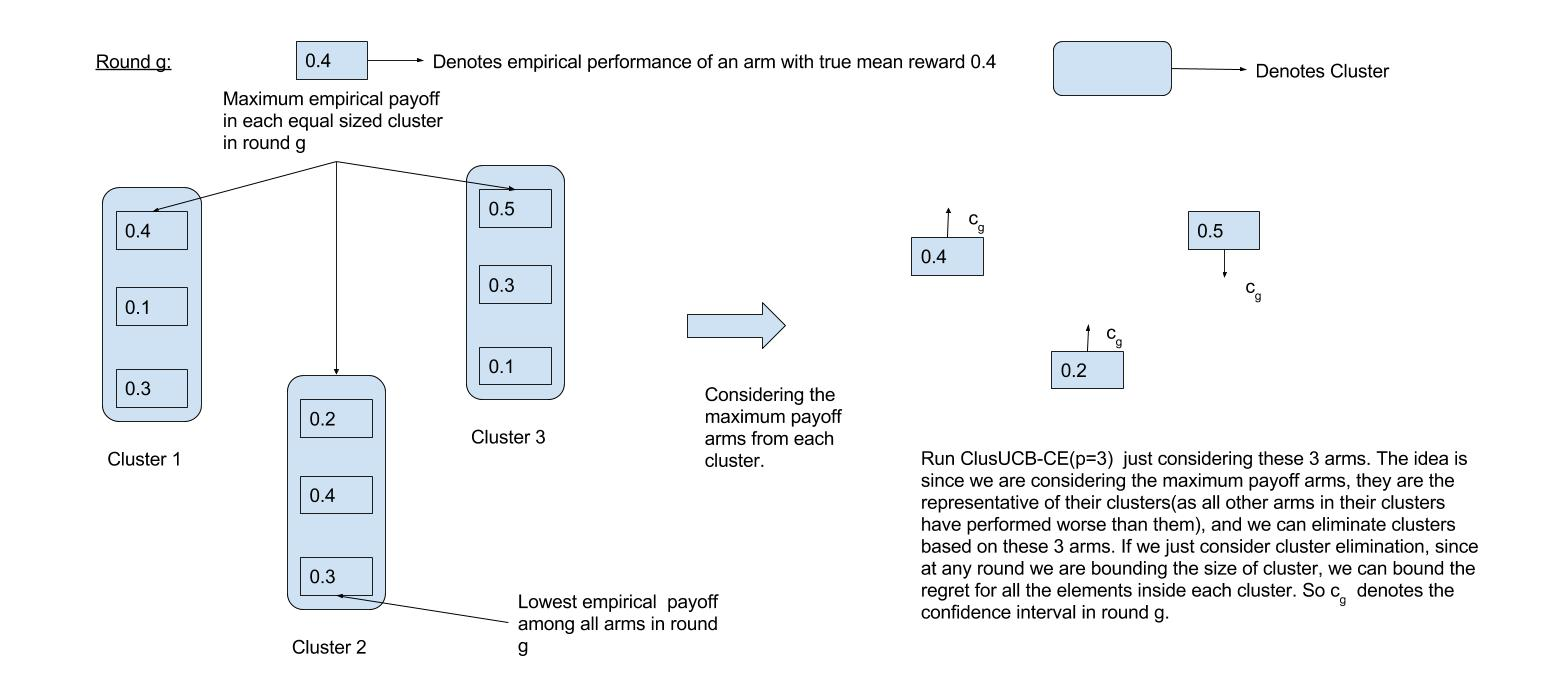
\includegraphics[scale=0.3]{img/diagCluster.jpg}
\caption{Cluster Elimination}
\label{Fig:ClusFig}
\end{figure}

%\begin{proposition}
%Considering only the cluster elimination condition and $p>1$, the total regret till $T$ is upper bounded by $\E [R_{T}]\leq \sum\limits_{i\in A:\Delta_{i}\geq b}\bigg\lbrace \bigg(\dfrac{2^{2+4\rho_{s}}\rho_{s}^{2\rho_{s}}T^{1-\rho_{s}}}{\psi^{\rho_{s}}\Delta_{i}^{4\rho_{s}-1}}\bigg) + \bigg(\Delta_{i}+\dfrac{32\rho_{s}\log{(\psi T\dfrac{\Delta_{i}^{4}}{16\rho_{s}^{2}})}}{\Delta_{i}}\bigg)  +  \bigg(\dfrac{T^{1-\rho_{s}}\rho_{s}^{2\rho_{s}}2^{2\rho_{s}+3}}{\psi^{\rho_{s}}\Delta_{i}^{4\rho_{s} -1}} \bigg)\bigg \rbrace +\sum\limits_{i\in A:0\leq\Delta_{i}\leq b}\bigg(\dfrac{T^{1-\rho_{s}}\rho_{s}^{2\rho_{s}}2^{2\rho_{s}+3}}{\psi^{\rho_{s}}b^{4\rho_{s} -1}} \bigg) + max_{i:\Delta_{i}\leq b}\Delta_{i}T$ for all $b\geq \sqrt{\dfrac{e}{T}}$, where $\rho_{s}\in (0,1]$ is the cluster elimination parameter, $\psi$ is the exploration regulatory factor, $p$ is the number of clusters and $T$ is the horizon.
%\end{proposition}

An illustrative diagram explaining Cluster Elimination is given in \textbf{Figure \ref{Fig:ClusFig}}. A slight modification to the algorithm allows us to do cluster elimination without any arm elimination. By taking $p>1$, removing the arm elimination condition, stopping when we are just left with one cluster and pulling the $max\lbrace \hat{r}_{i}\rbrace$, where ${i}\in B_{m}$ we can achieve this. We also take $\rho_{s}\in (0,1]$ as a constant in this proof whereby in Corollary \ref{Result:Corollary:1} and \ref{Result:Corollary:2} we use the different definitions. The theoretical analysis remains same as we have always bounded the values of $\rho_{s}\in (0,1]$.
 

\begin{proof}
% A sketch of the proof is given below,
%
%\begin{itemize}
%\item Define $C_{g}$ as the active cluster set which contains the max payoff arm from all the clusters active in the $g$-th round. So, the maximum cardinality of $C_{g}$ is $p$ and also this is always a non-increasing set.
%\item Now, the elements in $C_{g}$ which are the max-payoff arm from each cluster(if there are more than $1$ max-payoff arm in a cluster then choose randomly between them) are not fixed and hence like $B_{m}$ in proposition \ref{proofTheorem:Prop:1} cannot be tied to an arm $a_{i}$ throughout the rounds. For this purpose the $i$-th element in $C_{g}$ we tie to a cluster, that is $a_{\max_{s_{k}}}\in C_{g}$ is the max payoff arm in the cluster $s_{k}$ if the cluster $s_{k}$ still surviving in round $g$ and call $a_{\max_{s_{k}}}$ as a cluster arm. 
%\item Define $g$-th round(like in proposition \ref{proofTheorem:Prop:1}) as the same way as the $m$-th round signifying the first/minimum round when a cluster gets eliminated.
%%\item Let in the $g$-th round $C_{g}$ be the set which contains all the max payoff arms from each cluster.
%\item For regret bound proof according to proposition \ref{proofTheorem:Prop:1}, consider only this $C_{g}$ and proof following the same way as in proposition \ref{proofTheorem:Prop:1} with some changes. In any round $g$, atleast one of these $5$ events must occur:-
%\begin{itemize}
%\item \textbf{Case a1:} $a^{*}\in C_{g}$ and bound the regret that a sub-optimal cluster arm $a_{\max_{s_{k}}}\in C_{g}$ does not get eliminated on or before $g_{s_{k}}$-th round.
%\item \textbf{Case a2:} $a^{*}\notin C_{g}$ and bound the regret that a sub-optimal cluster arm $a_{\max_{s_{k}}}$ does not get eliminated on or before $a_{max_{s^{*}}}\in C_{g}$, such that $a_{\max_{s^{*}}},a^{*}\in s^{*}$ and $a_{\max_{s^{*}}}\neq a^{*}$. So, $a^{*}$ survives by this condition.
%\item \textbf{Case b1:} Cluster arm $a_{s_{k}}$ gets eliminated on $g_{s_{k}}$-th round(or before) with $a^{*}$ still in $B_{g_{s_{k}}}$ and calculate the regret for the arm pulls for all arms in cluster $s_{k}$(clusters are fixed).
%\item \textbf{Case b2:} $a^{*}\in C_{g}$ and $s^{*}$ gets eliminated by another sub-optimal cluster arm and bound this regret.
%\item \textbf{Case b3:} $a^{*}\notin C_{g}$ and $s^{*}$ gets eliminated by another sub-optimal cluster arm  and bound this regret.
%\end{itemize}
%For bounding the regret we use Chernoff-Hoeffding bound and use it on the current set of cluster arms $a_{max_{s_{k}}}\in C_{g},\forall s_{k}\in S$. This will work because of the algorithm, we are pulling all the  surviving arms equal number of times in each round and applying the same confidence interval for cluster elimination to all of the elements of $C_{g}$ and also we fix the clusters from beginning of the rounds.
%%Hence, $C_{g}$ actually behaves like the set $B_{m}$ in proposition $5$ but contains just the max payoff arm from each cluster.
%\item Introduce a constant $\rho_{s}\in (0,1]$ for cluster elimination to mimic the arm elimination condition in proposition \ref{proofTheorem:Prop:1}, but with the condition that whenever $\sqrt{\rho_{s}\epsilon_{g_{s_{k}}}} <  \dfrac{\Delta_{a_{\max_{s_{k}}}}}{2}, a_{\max_{s_{k}}}\in C_{g}$, then the cluster $s_{k}$(where 
%$\hat{r}_{a_{\max_{s_{k}}}}$ is the max payoff) gets eliminated. Because of the algorithm, we are guaranteed that the  maximum size of the cluster in the $g$-th round is $\ell=\bigg\lceil \dfrac{K}{p}\bigg\rceil$.
%\end{itemize}

Let $C_{g_{s_{k}}}=\lbrace \hat{r}_{a_{\max_{s_{k}}}} | \forall s_{k}\in S \rbrace$, that is let $C_{g_{s_{k}}}$ be the set of all arms which has the maximum estimated payoff arms from their respective clusters in the $g_{s_{k}}$-th round.  
Let, for each sub-optimal cluster arm $a_{\max_{s_{k}}}\in C_{g_{s_{k}}}$, $g_{s_{k}}=\min{\lbrace g|\sqrt{\rho_{s}\epsilon_{g}} < \dfrac{\Delta_{a_{\max_{s_{k}}}}}{2} \rbrace}$. So, $g_{s_{k}}$ be the first round when $\sqrt{\rho_{s}\epsilon_{g_{s_{k}}}} < \dfrac{\Delta_{a_{\max_{s_{k}}}}}{2}$ where $a_{\max_{s_{k}}}\in C_{g_{s_{k}}}$ is the maximum payoff arm in cluster $s_{k}$. Here, $a_{\max_{s_{k}}}$ is called cluster arm. Here, $A_{{s_{k}}}$ denotes the arm set in the cluster $s_{k}$. Let $A_{s_{k}}^{'}=\lbrace i\in A_{s_{k}}: \Delta_{i}> b\rbrace$, $A_{s_{k}}^{''}=\lbrace i\in A_{s_{k}}: \Delta_{i} > 0\rbrace$, $A^{'}=\lbrace i\in A: \Delta_{i}> b\rbrace$ and $A^{''}=\lbrace i\in A: \Delta_{i} > 0\rbrace$.

%The parameter $\rho_{s}$ is introduced just to make sure that the cluster elimination is a more aggressive elimination than arm elimination.
\subsection*{Case a: \textit{ Some sub-optimal cluster arm $a_{max_{s_{k}}}$ is not eliminated in round $g_{s_{k}}$ or before with $* \in C_{g_{s_{k}}}$ }}
%\subsubsection*{Case a1: \textit{ Some sub-optimal cluster arm $a_{max_{s_{k}}}$ is not eliminated in round $g_{s_{k}}$ or before and the optimal cluster arm $a^{*}\in C_{g_{s_{k}}} \subset B_{m}$ }}

%	In arm elimination condition, given the choice of confidence interval $c_{g_{s_{k}}}=\sqrt{\dfrac{\rho_{s} \log (\psi T\epsilon_{g_{s_{k}}}^{2})}{2 n_{g_{s_{k}}}}}$, we want to bound the probability of the event $\hat{r}_{s_{k}}+c_{g_{s_{k}}}\geq \hat{r}^{*}-c_{g_{s_{k}}}$.
%with a more tighter event of $ \hat{r}_{i} + \sqrt{w_{s_{k}}}c_{m} \leq \hat{r}^{*} - \sqrt{w_{s_{k}}}c_{m}$ which will result in faster elimination of arms within a cluster, given the choice of $c_{m}$ and $w_{s_{k}}$.
  %Now, $c_{g_{s_{k}}}=\sqrt{\dfrac{\rho_{s} \log (\psi T\epsilon_{g_{s_{k}}}^{2})}{2 n_{g_{s_{k}}}}}$, where $0 < \rho_{s}\leq 1$.
  
	Following the steps of Theorem \ref{Result:Theorem:1} Case $a2$, an arbitrary sub-optimal arm ${i}\in A^{'}$ can get eliminated only when the event,
	\begin{align}
	\hat{r}_{a_{\max_{s_{k}}}}  \le r_{a_{\max_{s_{k}}}} + c_{m_{i}} \text{ and } \label{eq:appB:armelim-casea}
 	\hat{r}^{*}\geq  r^{*} - c_{m_{i}}
	\end{align}
	
	takes place. So to bound the regret we need to bound the probability of the complementary event of these two conditions.  
  
  
  Putting the value of $n_{g_{s_{k}}}=\dfrac{2\log{(\psi T\epsilon_{g_{s_{k}}}^{2})}}{\epsilon_{g_{s_{k}}}}$ in $c_{g_{s_{k}}}$ we get,
  \begin{align*}
  c_{g_{s_{k}}}= & \sqrt{\dfrac{\rho_{s}*\epsilon_{g_{s_{k}}}\log (\psi  T\epsilon_{g_{s_{k}}}^{2})}{2*2 \log(\psi T\epsilon_{g_{s_{k}}}^{2})}}\\
  &=\sqrt{\dfrac{\rho_{s}\epsilon_{g_{s_{k}}}}{2}}\\
  &=\sqrt{\rho_{s}\epsilon_{g_{s_{k}}+1}} < \dfrac{\sqrt{\rho_{s}}\Delta_{a_{\max_{s_{k}}}}}{4} < \dfrac{\Delta_{a_{\max_{s_{k}}}}}{4}
  \end{align*}
%  $c_{g_{s_{k}}}=\sqrt{\dfrac{\rho_{s}*\epsilon_{g_{s_{k}}}\log (\psi T\epsilon_{g_{s_{k}}}^{2})}{2*2 \log(\psi T\epsilon_{g_{s_{k}}}^{2})}}=\sqrt{\dfrac{\rho_{s}\epsilon_{g_{s_{k}}}}{2}} = \sqrt{\rho_{s}\epsilon_{g_{s_{k}}+1}} < \dfrac{\sqrt{\rho_{s}}\Delta_{a_{max_{s_{k}}}}}{4} < \dfrac{\Delta_{a_{max_{s_{k}}}}}{4} $

  Again, for $a_{\max_{s_{k}}}, * \in C_{g_{s_{k}}}$, 
  \begin{align*}
  \hat{r}_{a_{\max_{s_{k}}}} + c_{g_{s_{k}}}\leq r_{a_{\max_{s_{k}}}} + 2c_{g_{s_{k}}} &= \hat{r}_{a_{\max_{s_{k}}}} + 4c_{g_{k}} - 2c_{g_{s_{k}}}\\
  &< r_{a_{\max_{s_{k}}}} + \Delta_{a_{\max_{s_{k}}}} - 2c_{g_{s_{k}}}\\
  &= r^{*} -2c_{g_{s_{k}}}\\
  &\leq \hat{r}^{*} - c_{g_{s_{k}}}
  \end{align*}
   
%Hence, we get that as soon as $\sqrt{\rho_{s}\epsilon_{g_{s_{k}}}}<\dfrac{\Delta_{a_{max_{s_{k}}}}}{2}$, 
% 	$a_{max_{s_{k}}}\in C_{g_{s_{k}}}$ gets eliminated.
%  So, $\hat{r}_{i}+c_{m}\leq \hat{r}_{i}+2c_{m}\leq r_{i} + \Delta_{i} - 2\sqrt{w_{s_{k}}}c_{m}\leq r^{*} - 2\sqrt{w_{s_{k}}}c_{m}$
%\leq \hat{r}^{*} - \sqrt{w}c_{m}
%  $\Rightarrow\hat{r}_{i}+c_{m}\leq \hat{r}_{i} - \sqrt{w}c_{m}  \leq r^{*} - \sqrt{w}c_{m}$
%  $\Rightarrow \hat{r}_{i} \leq {r}^{*} - 2\sqrt{w_{s_{k}}}c_{m} - 2c_{m} \leq \hat{r}^{*} - 2\sqrt{w_{s_{k}}}c_{m}$
%	So, we need to bound the probability of the event of $\hat{r}_{a_{max_{s_{k}}}}+c_{g_{s_{k}}}\geq \hat{r}^{*}-c_{g_{s_{k}}}$.
  %given that $\sqrt{\rho_{s}\epsilon_{g_{s_{k}}}}<\dfrac{\Delta_{a_{max_{s_{k}}}}}{2}$ becomes true for some arm $a_{max_{s_{k}}}\in C_{g_{s_{k}}}$ after the $g$-th round and $c_{g_{s_{k}}}=\sqrt{\dfrac{\rho_{s} \log (\psi T\epsilon_{g_{s_{k}}}^{2})}{2 n_{g_{s_{k}}}}}$.
%  $\Rightarrow \hat{r}_{i}+2c_{m}\leq \hat{r}_{i} + 2\sqrt{w}c_{m} \leq \hat{r}^{*}$
%  $\Rightarrow \hat{r}_{i} + \sqrt{w}c_{m} \leq \hat{r}^{*} - \sqrt{w}c_{m}$
%  $\Rightarrow\hat{r}_{i}+c_{m}\sqrt{\dfrac{w\ell_{m}}{\epsilon_{m}}} \leq \hat{r}^{*}-c_{m}\sqrt{\dfrac{w\ell_{m}}{\epsilon_{m}}} $, as $c_{m}\sqrt{\dfrac{w\ell_{m}}{\epsilon_{m}}} > 0$

%\begin{proof} of Proposition 2:
% 
%Now, we can bound $\hat{r}_{i}+c_{m}\leq \hat{r}^{*}-c_{m}$ given that $\sqrt{\epsilon_{m}}<\dfrac{\Delta_{i}}{2}$ for some arm $a_{i}\in s_{k}$. 
%	So, we need to bound the probability,
%	\begin{align*}
%	&\mathbb{P}\lbrace\hat{r}^{*}\leq r^{*} - c_{g_{s_{k}}}\rbrace\leq U_{g}\text{, where $U_{g}$ is an  arbitrary upper bound.}
%	\end{align*}

	Applying Chernoff-Hoeffding bound and considering independence of complementary of the two events in \ref{eq:appB:armelim-casea},
 
 \begin{align*}
 \mathbb{P}\bigg\lbrace\hat{r}^{*} \leq r^{*} - c_{g_{s_{k}}}\bigg\rbrace&\leq exp(-2c_{g_{s_{k}}}^{2}n_{g_{s_{k}}})\\
 &\leq exp(-2 * \dfrac{\rho_{s}\log ( \psi T\epsilon_{g_{s_{k}}}^{2})}{2 n_{g_{s_{k}}}} *n_{g_{s_{k}}})\\
 &\leq \dfrac{1}{(\psi T\epsilon_{g_{k}}^{2})^{\rho_{s}}}
 \end{align*}
% \hspace*{0em} $\mathbb{P}\lbrace\hat{r}^{*}\leq r^{*} - c_{g_{s_{k}}}\rbrace\leq exp(-2c_{g_{s_{k}}}^{2}n_{g_{s_{k}}})$
% \hspace*{8em} $\leq exp(-2 * \dfrac{\rho_{s}\log ( \psi T\epsilon_{g_{s_{k}}}^{2})}{2 n_{g_{s_{k}}}} *n_{g_{s_{k}}})$
% \hspace*{8em} $\leq \dfrac{1}{(\psi T\epsilon_{g_{k}}^{2})^{\rho_{s}}}$

 
Similarly, $\mathbb{P}\bigg\lbrace\hat{r}_{a_{max_{s_{k}}}}\geq r_{a_{max_{s_{k}}}} + c_{g_{s_{k}}}\bigg\rbrace\leq \dfrac{1}{(\psi T\epsilon_{g_{s_{k}}}^{2})^{\rho_{s}}}$
 
Summing, the two up, the probability that a sub-optimal cluster arm $a_{max_{s_{k}}}\in C_{g_{s_{k}}}$ is not eliminated in $g_{s_{k}}$-th round is  $\bigg(\dfrac{2}{(\psi  T\epsilon_{g_{s_{k}}}^{2})^{\rho_{s}}}\bigg)$. 
  Now, for each round $g_{s_{k}}$, all the elements of $C_{g_{s_{k}}}$ are the respective max payoff arms of their cluster $s_{k}$, that is all the other arms in their respective clusters have performed worse than them. Hence, since $A_{s_{k}}^{'}\supset C_{g_{s_{k}}}$, we are pulling all the surviving arms equally in each round and since clusters are fixed so we can bound the maximum probability that a sub-optimal arm ${j}\in A^{'}_{s_{k}}$  and ${j}\in s_{k}$ such that $a_{max_{s_{k}}}\in C_{g_{s_{k}}}$ is not eliminated on or before the $g_{s_{k}}$-th round by the same probability of 
  
  %, \forall s_{k}\in S_{g_{s_{k}}}
\begin{align*}
\bigg(\dfrac{2}{(\psi T\epsilon_{g_{s_{k}}}^{2})^{\rho_{s}}}\bigg)
\end{align*}  
 
 
Summing up over all arms in $s_{k}$ and bounding the regret trivially by $T\Delta_{i}$,
\begin{align*}
\sum_{i\in A_{s_{k}}^{'}}\bigg(\dfrac{2T\Delta_{i}}{(\psi T\epsilon_{g_{s_{k}}}^{2})^{\rho_{s}}}\bigg)
\end{align*}

 
Summing up over all $p$ clusters and bounding the regret for each arm $i\in A_{s_{k}}^{'} $ trivially by $T\Delta_{i}$,
 \begin{align*}
 \sum_{k=1}^{p}\sum_{i\in A_{s_{k}}^{'}}\bigg(\dfrac{2T\Delta_{i}}{(\psi T\dfrac{\Delta_{i}^{4}}{16\rho_{s}^{2}})^{\rho_{s}}}\bigg) &= \sum_{i\in A^{'}}\bigg(\dfrac{2T\Delta_{i}}{(\psi  T\dfrac{\Delta_{i}^{4}}{16\rho_{s}^{2}})^{\rho_{s}}}\bigg) \\
 &\leq \sum_{i\in A^{'}}\bigg(\dfrac{2^{1+4\rho_{s}}T^{1-\rho_{s}}\rho_{s}^{2\rho_{s}}\Delta_{i}}{\psi^{\rho_{s}}\Delta_{i}^{4\rho_{s}}}\bigg)\\
 &\leq \sum_{i\in A^{'}}\bigg(\dfrac{2^{1+4\rho_{s}}\rho_{s}^{2\rho_{s}}T^{1-\rho_{s}}}{\psi^{\rho_{s}}\Delta_{i}^{4\rho_{s}-1}}\bigg)\\
 &= \sum_{i\in A^{'}}\bigg(\dfrac{C_{1}(\rho_{s})T^{1-\rho_{s}}}{\Delta_{i}^{4\rho_{s}-1}}\bigg) \text{, where } C_1(x) = \frac{2^{1+4x}x^{2x}}{\psi^{x}}
 \end{align*}
 
% \hspace*{4em} $\sum_{k=1}^{p}\sum_{i\in A_{s_{k}}}\bigg(\dfrac{2T\Delta_{i}}{(\psi T\dfrac{\Delta_{i}^{4}}{16\rho_{s}^{2}})^{\rho_{s}}}\bigg)$
% \hspace*{4em} $\sum_{i\in A}\bigg(\dfrac{2T\Delta_{i}}{(\psi T\dfrac{\Delta_{i}^{4}}{16\rho_{s}^{2}})^{\rho_{s}}}\bigg)\leq \sum_{i\in A}\bigg(\dfrac{2^{1+4\rho_{s}}T^{1-\rho_{s}}\rho_{s}^{2\rho_{s}}\Delta_{i}}{\psi^{\rho_{s}}\Delta_{i}^{4\rho_{s}}}\bigg)$
% \hspace*{14em}
%$\leq \sum_{i\in A}\bigg(\dfrac{2^{1+4\rho_{s}}\rho_{s}^{2\rho_{s}}T^{1-\rho_{s}}}{\psi^{\rho_{s}}\Delta_{i}^{4\rho_{s}-1}}\bigg)$

%\subsubsection*{Case a2: \textit{ Some sub-optimal cluster arm $a_{max_{s_{k}}}$ is not eliminated in round $g_{s_{k}}$ or before and the optimal cluster arm $a^{*}\notin C_{g_{s_{k}}} \subset B_{m}$ }}
%%\textbf{Case a2:} Some sub-optimal cluster arm $a_{max_{s_{k}}}$ is not eliminated in round $g_{s_{k}}$ or before and the optimal cluster arm $a^{*}\notin C_{g_{s_{k}}} \subset B_{m}$. 
%	
%	In the above case we considered that $a^{*}\in C_{g_{s_{k}}}$ being the max-payoff arm from optimal cluster $s^{*}$. Now, if that is not the case and $\exists a_{\max_{s^{*}}}\in s^{*}$ such that $\hat{r}_{a_{\max_{s^{*}}}}> \hat{r}^{*}$, so $a_{\max_{s^{*}}}$ will be in $C_{g_{s_{k}}}$ in the $g_{s_{k}}$-th round. In this case for some sub-optimal arm $a_{max_{s_{k}}}\in C_{g_{s_{k}}}$, we have to bound the probability
%	\begin{align*}
%	&\mathbb{P}\bigg\lbrace\hat{r}_{a_{\max_{s_{k}}}}+c_{g_{s_{k}}}\bigg\rbrace< \mathbb{P}\bigg\lbrace\hat{r}_{a_{\max_{s^{*}}}}-c_{g_{s_{k}}}\bigg\rbrace
%	\end{align*}		 
%	 
%	 
%	 But, this probability can be no worse than case a1 since $r_{\max_{s^{*}}} < r^{*}$ and all arms get pulled $n_{g_{s_{k}}}$ number of times in the $g$-th round. So the regret for not eliminating a sub-optimal cluster even when $a^{*}\notin C_{g_{s_{k}}}$(but still surviving in $s^{*}$) can be no worse than,
%	 \begin{align*} 
%	 \bigg(\dfrac{2}{(T\epsilon_{g_{s_{k}}}^{2})^{\rho_{s}}}\bigg) 
%	 \end{align*}
%	 After summing over all arms in $A$ and bounding 
%trivially by $T\Delta_{i}$ we get the same result as above we can show that the regret can be no more than,
% \begin{align*}
% &\sum_{i\in A^{'}}\bigg(\dfrac{2^{1+4\rho_{s}}\rho_{s}^{2\rho_{s}}T^{1-\rho_{s}}}{\psi^{\rho_{s}}\Delta_{i}^{4\rho_{s}-1}}\bigg)=\sum_{i\in A^{'}}\bigg(\dfrac{C_{1}(\rho_{s})T^{1-\rho_{s}}}{\Delta_{i}^{4\rho_{s}-1}}\bigg)
% \end{align*}
%%$\sum_{i\in A}\bigg(\dfrac{2^{1+4\rho_{s}}\rho_{s}^{2\rho_{s}}T^{1-\rho_{s}}}{\psi^{\rho_{s}}\Delta_{i}^{4\rho_{s}-1}}\bigg)$


\subsection*{Case b: \textit{For each arm $i$, either ${i}$ is eliminated in round $g_{s_{k}}$ or before or there is no optimal arm ${*}$ in $C_{g_{s_{k}}}$ }}

\subsubsection*{Case b1: \textit{${*}\in C_{g_{s_{k}}}$ for each arm $i \in A'$ and cluster $s_{k}$ eliminated on or before $g_{s_{k}}$} }
	
	Again, in the $g_{s_{k}}$-th round, the maximum total elements in the cluster $s_{k}$ can be no more than $\ell=\bigg\lceil \dfrac{K}{p}\bigg\rceil$.
 
Also, since we are eliminating a sub-optimal cluster arm $a_{\max_{s_{k}}}\in C_{g_{s_{k}}}$ on or before round $g_{s_{k}}$, it is pulled (along with all the other arms in that cluster) no longer than,
 \begin{align*}
 &n_{g_{s_{k}}}=\bigg\lceil\dfrac{2\log{(\psi T\epsilon_{g_{s_{k}}}^{2})}}{\epsilon_{g_{s_{k}}}}\bigg\rceil
 \end{align*}

So, the total contribution of $a_{\max_{s_{k}}}$  along with all the other arms in the cluster till round $g_{s_{k}}$ is given by,
 \begin{align*}
 &\sum_{i\in A_{s_{k}}}\Delta_{i}\bigg\lceil\dfrac{2\log{(\psi T\epsilon_{g_{s_{k}}}^{2})}}{\epsilon_{g_{s_{k}}}}\bigg\rceil\\
 &\leq\sum_{i\in A_{s_{k}}^{'}}\Delta_{i}\bigg\lceil\dfrac{2\log{(\psi T(\dfrac{\Delta_{i}}{2\sqrt{\rho_{s}}})^{4})}}{(\dfrac{\Delta_{i}}{2\sqrt{\rho_{s}}})^{2}}\bigg\rceil \text{, since }\sqrt{\rho_{s}\epsilon_{g_{s_{k}}}} <\dfrac{\Delta_{a_{max_{s_{k}}}}}{2} <  \dfrac{\Delta_{i}}{2} \text{, as } {r}_{a_{max_{s_{k}}}}>{r}_{i},\forall i\in s_{k}\\
 &\leq\sum_{i\in A_{s_{k}}^{'}}\Delta_{i}\bigg(1+\dfrac{32*\rho_{s}*\log{(\psi T(\dfrac{\Delta_{i}}{2\sqrt{\rho_{s}}})^{4})}}{\Delta_{i}^{2}}\bigg)\\
 &\leq\sum_{i\in A_{s_{k}}^{'}}\Delta_{i}\bigg(1+\dfrac{32\rho_{s}\log{(\psi T\dfrac{\Delta_{i}^{4}}{16\rho_{s}^{2}})}}{\Delta_{i}^{2}}\bigg)
 \end{align*}

 
Summing over all $p$ clusters the total regret is given by,
 
\begin{align*}
&\sum_{k=1}^{p}\sum_{i\in A_{s_{k}}^{'}}\Delta_{i}\bigg(1+\dfrac{32\rho_{s}\log{(\psi  T\dfrac{\Delta_{i}^{4}}{16\rho_{s}^{2}})}}{\Delta_{i}^{2}}\bigg)\\
&\leq\sum_{i\in A^{'}}\Delta_{i}\bigg(1+\dfrac{32\rho_{s}\log{(\psi T\dfrac{\Delta_{i}^{4}}{16\rho_{s}^{2}}})}{\Delta_{i}^{2}}\bigg)
\end{align*}


\subsubsection*{Case b2: \textit{$s^{*}$ is eliminated by some sub-optimal cluster.} } 
	
	Let $C_{g}^{'}=\lbrace a_{max_{s_{k}}}\in A^{'}|\forall s_{k}\in S \rbrace$ and $C_{g}^{''}=\lbrace a_{max_{s_{k}}}\in A^{''}|\forall s_{k}\in S \rbrace$. Firstly, if conditions of case $b1$ holds then the optimal arm ${*}\in C_{g_{s_{k}}}$ will not be eliminated in round $g_{s_{k}}=g_{*}$ or it will lead to the contradiction that $r_{a_{\max_{s_{k}}}}>r^{*}$ where $a_{\max_{s_{k}}},{*}\in C_{g_{s_{k}}}$. In any round $g_{*}$, if the optimal arm ${*}$ gets eliminated then for any round from $1$ to $g_{s_{j}}$ all arms $a_{\max_{s_{j}}}\in C_{g_{s_{k}}},\forall s_{j}\neq s^{*}$ such that $g_{s_{j}}< g_{*}$ were eliminated according to assumption in Case $a$. Let, the arms surviving till $g_{*}$ round be denoted by $C_{g}^{'}$. This leaves any arm $a_{s_{b}}$ such that $g_{s_{b}}\geq g_{*}$ to still survive and eliminate arm ${*}$ in round $g_{*}$. Let, such arms that survive ${*}$ belong to $C_{g}^{''}$. Also maximal regret per step after eliminating ${*}$ is the maximal $\Delta_{a_{\max_{s_{j}}}}$ among the remaining arms ${a_{\max_{s_{j}}}}\in C_{g_{s_{j}}}$ with $g_{s_{j}}\geq g_{*}$. Hence, the maximal regret after eliminating the arm ${*}$ is upper bounded by, 
 \begin{align*}
 &\sum_{g_{*}=0}^{max_{a_{\max_{s_{j}}}\in C_{g}^{'}}g_{s_{j}}}\sum_{\substack{a_{\max_{s_{k}}}\in C_{g}^{''}: \\ g_{s_{k}} \geq g_{*}}}\bigg(\dfrac{2}{(\psi T\epsilon_{g_{s^{*}}}^{2})^{\rho_{s}}} \bigg).T\max_{\substack{a_{\max_{s_{j}}}\in C_{g}^{''}: \\ g_{s_{j}}\geq g_{*}}}{\Delta}_{a_{\max_{s_{j}}}}
 \end{align*}
%Let $g_{s_{b}}=\min\lbrace g|\sqrt{\rho_{s}\epsilon_{g}}<\dfrac{\Delta_{a_{\max_{s_{b}}}}}{2}\rbrace$.
But, we know that for any round $g$, elements of $C_{g}$ are the best performers in their respective clusters. So, taking that into account and $A'\supset C_{g}^{'}$ and $A''\supset C_{g}^{''}$ the regret can be bounded by,
%\text{, since }\sqrt{\rho_{s}\epsilon_{g_{s_{j}}}} < \dfrac{\Delta_{j}}{2} <  \dfrac{\Delta_{j}}{2} \text{, as }{r}_{a_{s_{j}}}>{r}_{j},\forall j\in s_{j}
\begin{align*}
 & \sum_{g_{*}=0}^{max_{j\in A^{'}\setminus A_{s^*}^{'}}g_{s_{j}}}\sum_{i\in A^{''}\setminus A_{s^*}^{'}:g_{s_{k}}>g_{*}}\bigg(\dfrac{2}{(\psi T\epsilon_{g_{s_{k}}}^{2})^{\rho_{s}}} \bigg).T\max_{j\in A^{''}:g_{s_{j}}\geq g_{*}}{\Delta}_{j}\\
 &\leq\sum_{g_{*}=0}^{max_{j\in A^{'}\setminus A_{s^*}^{'}}g_{s_{j}}}\sum_{i\in A^{''}\setminus A_{s^*}^{'}:g_{s_{k}}>g_{*}}\bigg(\dfrac{2}{(\psi T\epsilon_{g_{s_{k}}}^{2})^{\rho_{s}}} \bigg).T.2\sqrt{\rho_{s}\epsilon_{g_{s_{j}}}}\\
 &\leq\sum_{g_{*}=0}^{max_{j\in A^{'}\setminus A_{s^*}^{'}}g_{s_{j}}}\sum_{i\in A^{''}\setminus A_{s^*}^{'}:g_{s_{k}}>g_{*}}\bigg(\dfrac{4T^{1-\rho_{s}}}{\psi^{\rho_{s}}\epsilon_{g_{s_{k}}}^{2\rho_{s} - \frac{1}{2}}} \bigg)\\
 &\leq\sum_{i\in A^{''}\setminus A_{s^*}^{'}:g_{s_{k}}>g_{*}}\sum_{g_{*}=0}^{\min{\lbrace g_{s_{k}},g_{s_{b}}\rbrace}}\bigg(\dfrac{4T^{1-\rho_{s}}}{\psi^{\rho_{s}}2^{({2\rho_{s} - \frac{1}{2}})g_{*}}} \bigg) \\
 &\leq\sum_{i\in A^{'}\setminus A_{s^*}^{'}}\bigg(\dfrac{4T^{1-\rho_{s}}}{\psi^{\rho_{s}}2^{({2\rho_{s} - \frac{1}{2}})g_{*}}} \bigg)+\sum_{i\in A^{''}\setminus A^{'}\cup A_{s^*}^{'}}\bigg(\dfrac{4T^{1-\rho_{s}}}{\psi^{\rho_{s}}2^{({2\rho_{s} - \frac{1}{2}})g_{s_{b}}}} \bigg)\\ 
 &\leq\sum_{i\in A^{'}\setminus A_{s^*}^{'}}\bigg(\dfrac{4\rho_{s}^{2\rho_{s}}T^{1-\rho_{s}}*2^{2\rho_{s}-\frac{1}{2}}}{\psi^{\rho_{s}}\Delta_{i}^{4\rho_{s}-1}} \bigg)+\sum_{i\in A^{''}\setminus A^{'}\cup A_{s^*}^{'}}\bigg(\dfrac{4\rho_{s}^{2\rho_{s}}T^{1-\rho_{s}}*2^{2\rho_{s}-\frac{1}{2}}}{\psi^{\rho_{s}}b^{4\rho_{s}-1}} \bigg)\\
 &\leq\sum_{i\in A^{'}\setminus A_{s^*}^{'}}\bigg(\dfrac{T^{1-\rho_{s}}\rho_{s}^{2\rho_{s}}2^{2\rho_{s}+\frac{3}{2}}}{\psi^{\rho_{s}}\Delta_{i}^{4\rho_{s}-1}} \bigg)+\sum_{i\in A^{''}\setminus A^{'}\cup A_{s^*}^{'}}\bigg(\dfrac{T^{1-\rho_{s}}\rho_{s}^{2\rho_{s}}2^{2\rho_{s}+\frac{3}{2}}}{\psi^{\rho_{s}}b^{4\rho_{s}-1}} \bigg)\\
 & = \sum_{i\in A^{'}\setminus A_{s^*}^{'}}\bigg(\dfrac{C_{2}(\rho_{s})T^{1-\rho_{s}}}{\Delta_{i}^{4\rho_{s}-1}} \bigg)+\sum_{i\in A^{''}\setminus A^{'}\cup A_{s^*}^{'}}\bigg(\dfrac{C_{2}(\rho_{s})T^{1-\rho_{s}}}{b^{4\rho_{s}-1}} \bigg) \text{, where } C_2(x) = \frac{2^{2x+\frac{3}{2}}x^{2x}}{\psi^{x}}
\end{align*}

\subsubsection*{Case b3: \textit{${*}$ is not in $C_{g_{s_{k}}}$, but belongs to $B_{g_{s_{k}}}$} } 

In this case the optimal arm ${*}\in s^{*}$ is not eliminated, also $s^{*}$ is not eliminated. So, for all sub-optimal arms $i$ in $A'$ which gets eliminated on or before $g_{s_{k}}$ will get pulled no less than $\bigg\lceil\dfrac{2\log{(\psi T\epsilon_{g_{s_{k}}}^{2})}}{\epsilon_{g_{s_{k}}}}\bigg\rceil$ number of times, which leads to the following bound the contribution to the expected regret, as in Case $b1$:
% 
% \begin{align*}
%  &\sum_{i\in A^{'}}\Delta_{i}\bigg\lceil\dfrac{2\log{(\psi T\epsilon_{m_{i}}^{2})}}{\epsilon_{m_{i}}}\bigg\rceil
% \end{align*}
% Since $a^{*}$ is definitely in $B_{\max(m_{i},g_{s_{k}})}$ then following the same way as Case $b1$ we can show that can be no worse than,
\begin{align*}
 &\sum_{i\in A^{'}}\bigg\lbrace \Delta_{i}+\dfrac{32\rho_{s}\log{(\psi T\dfrac{\Delta_{i}^{4}}{16\rho_{s}^{2}})}}{\Delta_{i}} \bigg\rbrace 
\end{align*} 

For arms $a_i \notin s^*$, the contribution to the regret cannot be greater than that in Case $b2$. So the regret is bounded by,

\begin{align*}
\sum_{i\in A^{'}\setminus A_{s^*}^{'}}\dfrac{C_{2}(\rho_{s})T^{1-\rho_{s}}}{\Delta_{i}^{4\rho_{s}-1}} +\sum_{i\in A^{''}\setminus A^{'} \cup A_{s^*}^{'}}\dfrac{C_{2}(\rho_{s})T^{1-\rho_{s}}}{b^{4\rho_{s}-1}}
\end{align*}

%\subsubsection*{Case b3: \textit{Cluster $s^{*}$ containing the optimal arm ${*}$ is eliminated by a sub-optimal cluster and ${*}\notin C_{g}$}}
% 
%	Now, in the above case again we considered that ${*}$ is in $C_{g}$. In this case we will consider that the cluster $s^{*}$ containing the optimal arm ${*}$ was eliminated by another sub-optimal cluster and ${*}\notin C_{g}$. This will be the mirror case of Case $b2$ and since $s^{*}$ gets eliminated by $a_{s_{b}}$ such that $\sqrt{\rho_{s}\epsilon_{g_{s_{b}}}}\geq\dfrac{\Delta_{a_{s_{b}}}}{2}$ round $g_{*}$. Also maximal regret per step after eliminating ${*}$ is the maximal $\Delta_{j}$ among the remaining arms ${j}\in B_{m}$ with $g_{s_{j}}\geq g_{*}$. Following the same way above we can bound the regret as,
% 
%\begin{align*}
%&\sum_{i\in A^{'}}\bigg(\dfrac{T^{1-\rho_{s}}\rho_{s}^{2\rho_{s}}2^{2\rho_{s}+\frac{3}{2}}}{\psi^{\rho_{s}}\Delta_{i}^{4\rho_{s}-1}} \bigg)+\sum_{i\in A^{''}\setminus A^{'}}\bigg(\dfrac{T^{1-\rho_{s}}\rho_{s}^{2\rho_{s}}2^{2\rho_{s}+\frac{3}{2}}}{\psi^{\rho_{s}}b^{4\rho_{s}-1}} \bigg)\\
%& = \sum_{i\in A^{'}}\bigg(\dfrac{C_{2}(\rho_{s})T^{1-\rho_{s}}}{\Delta_{i}^{4\rho_{s}-1}} \bigg)+\sum_{i\in A^{''}\setminus A^{'}}\bigg(\dfrac{C_{2}(\rho_{s})T^{1-\rho_{s}}}{b^{4\rho_{s}-1}} \bigg)
%\end{align*}
 
Summing up \textbf{Case a} and \textbf{Case b}, the total regret till round $g$ is given by,
\begin{align*}
  R_{T} \leq &  \sum_{i\in A:\Delta_{i} > b}\bigg\lbrace\underbrace{\bigg(\dfrac{C_{1}(\rho_{s})T^{1-\rho_{s}}}{\Delta_{i}^{4\rho_{s}-1}}\bigg)}_{\text{case a}} + \underbrace{\bigg(2\Delta_{i}+\dfrac{64\rho_{s}\log{(\psi T\dfrac{\Delta_{i}^{4}}{16\rho_{s}^{2}})}}{\Delta_{i}} }_{\text{case b1+b3}} \bigg\rbrace
  \\&+ \underbrace{\sum_{i\in A\setminus A_{s^*}: \Delta_{i} > b}\bigg(\dfrac{2C_{2}(\rho_{s})T^{1-\rho_{s}}}{\Delta_{i}^{4\rho_{s} -1}} \bigg)}_{\text{case b2}} \bigg\rbrace  + \underbrace{\sum_{i\in A\setminus A_{s^*}:0 < \Delta_{i}\leq b}\bigg(\dfrac{2C_{2}(\rho_{s})T^{1-\rho_{s}}}{\Delta_{i}^{4\rho_{s} -1}} \bigg)}_{\text{case b2}}  + max_{i\in A:\Delta_{i}\leq b}\Delta_{i}T
\end{align*}

%R_{T} \leq &  \sum_{i\in A:\Delta_{i} > b}\bigg\lbrace\underbrace{\bigg(\dfrac{C_{1}(\rho_{s})T^{1-\rho_{s}}}{\Delta_{i}^{4\rho_{s}-1}}\bigg)}_{\text{case a}} + \underbrace{\bigg(2\Delta_{i}+\dfrac{32\rho_{s}\log{(\psi T\dfrac{\Delta_{i}^{4}}{16\rho_{s}^{2}})}}{\Delta_{i}} + \dfrac{32\rho_{a}\log{(\psi T\dfrac{\Delta_{i}^{4}}{16\rho_{a}^{2}})}}{\Delta_{i}}  \bigg) }_{\text{case b1+b3}} 
%  \\&+ \underbrace{\bigg(\dfrac{C_{2}(\rho_{s})T^{1-\rho_{s}}}{\Delta_{i}^{4\rho_{s} -1}} \bigg)}_{\text{case b2}} \bigg\rbrace  + \underbrace{\sum_{i\in A:0\leq\Delta_{i}\leq b}\bigg(\dfrac{C_{2}(\rho_{s})T^{1-\rho_{s}}}{\Delta_{i}^{4\rho_{s} -1}} \bigg)}_{\text{case b2}}  + max_{i:\Delta_{i}\leq b}\Delta_{i}T

%R_{T} \leq & \sum_{i\in A:\Delta_{i} > b}\bigg\lbrace\underbrace{\bigg(\dfrac{C_{1}(\rho_{s})T^{1-\rho_{s}}}{\Delta_{i}^{4\rho_{s}-1}}\bigg)}_{\text{case a1}} +  \underbrace{\bigg(\Delta_{i}+\dfrac{32\rho_{s}\log{(\psi T\dfrac{\Delta_{i}^{4}}{16\rho_{s}^{2}})}}{\Delta_{i}}\bigg)}_{\text{case b1}} \\
%	& + \underbrace{\bigg(\dfrac{C_{2}(\rho_{s})T^{1-\rho_{s}}}{\Delta_{i}^{4\rho_{s} -1}} \bigg)}_{\text{case b2}} 
%	+ \underbrace{\sum_{i\in A^{'}}\bigg\lbrace \Delta_{i}+\dfrac{32\rho_{a}\log{(\psi T\dfrac{\Delta_{i}^{4}}{16\rho_{a}^{2}})}}{\Delta_{i}} \bigg\rbrace}_{\text{case b3}}  + max_{i:\Delta_{i}\leq b}\Delta_{i}T\\
% \\& +\underbrace{\sum_{i\in A:0\leq\Delta_{i}\leq b}\bigg(\dfrac{2C_{2}(\rho_{s})T^{1-\rho_{s}}}{b^{4\rho_{s} -1}} \bigg)}_{\text{case b2+b3}}  
% \underbrace{\bigg(\dfrac{C_{2}(\rho_{s})T^{1-\rho_{s}}}{\Delta_{i}^{4\rho_{s} -1}} \bigg)}_{\text{case b3}}\bigg \rbrace+\underbrace{\sum_{i\in A:0\leq\Delta_{i}\leq b}\bigg(\dfrac{C_{2}(\rho_{s})T^{1-\rho_{s}}}{b^{4\rho_{s} -1}} \bigg)}_{\text{case b2}} \\
%    & + \underbrace{\sum_{i\in A:0\leq\Delta_{i}\leq b}\bigg(\dfrac{C_{2}(\rho_{s})T^{1-\rho_{s}}}{b^{4\rho_{s} -1}} \bigg)}_{\text{case b3}}
% \underbrace{\bigg(\dfrac{C_{1}(\rho_{s})T^{1-\rho_{s}}}{\Delta_{i}^{4\rho_{s}-1}}\bigg)}_{\text{case a2}} +
%  R_{T} \leq & \sum_{i\in A:\Delta_{i}\geq b}\bigg\lbrace\underbrace{\bigg(\dfrac{2^{1+4\rho_{s}}\rho_{s}^{2\rho_{s}}T^{1-\rho_{s}}}{\psi^{\rho_{s}}\Delta_{i}^{4\rho_{s}-1}}\bigg)}_{\text{case a1}} + \underbrace{\bigg(\dfrac{2^{1+4\rho_{s}}\rho_{s}^{2\rho_{s}}T^{1-\rho_{s}}}{\psi^{\rho_{s}}\Delta_{i}^{4\rho_{s}-1}}\bigg)}_{\text{case a2}} + \underbrace{\bigg(\Delta_{i}+\dfrac{32\rho_{s}\log{(\psi T\dfrac{\Delta_{i}^{4}}{16\rho_{s}^{2}})}}{\Delta_{i}}\bigg)}_{\text{case b1}} \\
%	& + \underbrace{\bigg(\dfrac{T^{1-\rho_{s}}\rho_{s}^{2\rho_{s}}2^{2\rho_{s}+\frac{3}{2}}}{\psi^{\rho_{s}}\Delta_{i}^{4\rho_{s} -1}} \bigg)}_{\text{case b2}} + \underbrace{\bigg(\dfrac{T^{1-\rho_{s}}\rho_{s}^{2\rho_{s}}2^{2\rho_{s}+\frac{3}{2}}}{\psi^{\rho_{s}}\Delta_{i}^{4\rho_{s} -1}} \bigg)}_{\text{case b3}}\bigg \rbrace+\underbrace{\sum_{i\in A:0\leq\Delta_{i}\leq b}\bigg(\dfrac{T^{1-\rho_{s}}\rho_{s}^{2\rho_{s}}2^{2\rho_{s}+\frac{3}{2}}}{\psi^{\rho_{s}}b^{4\rho_{s} -1}} \bigg)}_{\text{case b2}} \\
%   &	+ \underbrace{\sum_{i\in A:0\leq\Delta_{i}\leq b}\bigg(\dfrac{T^{1-\rho_{s}}\rho_{s}^{2\rho_{s}}2^{2\rho_{s}+\frac{3}{2}}}{\psi^{\rho_{s}}b^{4\rho_{s} -1}} \bigg)}_{\text{case b3}} + max_{i:\Delta_{i}\leq b}\Delta_{i}T\\
%  = & \sum\limits_{i\in A:\Delta_{i}\geq b}\bigg\lbrace\underbrace{\bigg(\dfrac{2^{2+4\rho_{s}}\rho_{s}^{2\rho_{s}}T^{1-\rho_{s}}}{\psi^{\rho_{s}}\Delta_{i}^{4\rho_{s}-1}}\bigg)}_{\text{case a1+a2}} + \underbrace{\bigg(\Delta_{i}+\dfrac{32\rho_{s}\log{(\psi T\dfrac{\Delta_{i}^{4}}{16\rho_{s}^{2}})}}{\Delta_{i}}\bigg)}_{\text{case b1}}  +  \underbrace{\bigg(\dfrac{T^{1-\rho_{s}}\rho_{s}^{2\rho_{s}}2^{2\rho_{s}+3}}{\psi^{\rho_{s}}\Delta_{i}^{4\rho_{s} -1}} \bigg)}_{\text{case b2+b3}}\bigg \rbrace \\
%  & +\underbrace{\sum\limits_{i\in A:0\leq\Delta_{i}\leq b}\bigg(\dfrac{T^{1-\rho_{s}}\rho_{s}^{2\rho_{s}}2^{2\rho_{s}+3}}{\psi^{\rho_{s}}b^{4\rho_{s} -1}} \bigg)}_{\text{case b2+b3}} + max_{i:\Delta_{i}\leq b}\Delta_{i}T  
  
  
\end{proof}





%\section{Proof of Theorem 1}
%\label{App:C}
%
%\begin{proof}
%The optimal cluster which contains $a^{*}$ is denoted by $s^{*}$. The subset of arms belonging to cluster $s_{k}$ is denoted by $A_{s_{k}}$ and similarly the subset of arms belonging to $s^{*}$ is denoted by $A_{s^{*}}$. Combining both the cases of Proposition \ref{proofTheorem:Prop:1} and Proposition \ref{proofTheorem:Prop:2} we can see that a sub-optimal arm $a_{i}$ can only be eliminated given that either $m_{i}$ or $g_{s_{k}}$s.t $\exists a_{i}\in s_{k}$ happens with $a^{*}\in s^{*}$ still surviving. In Proposition \ref{proofTheorem:Prop:1} we consider only arm elimination and in Proposition \ref{proofTheorem:Prop:2} we consider only cluster elimination. Also this proof we will consider $p>1$. So there will be slight modification from what we proved in proposition \ref{proofTheorem:Prop:1} with $p=1$. For random uniform allocation we will assume that each cluster $s_{k},\forall s_{k}\in S$, gets such an arm such that $r_{{max_{s_{k}}}}\geq r_{a_{i}},\forall i\in s_{k}$. Again, $r_{a^{*}}\geq r_{{max_{s_{k}}}}, \forall s_{k}\in S$. Here also we take $\rho_{a},\rho_{s}\in (0,1]$ as a constant in this proof whereby in Corollary \ref{Result:Corollary:1} and \ref{Result:Corollary:2} we use the different definitions. The theoretical analysis remains same as we have always bounded the values of $\rho_{a}\in (0,1]$(see Appendix \ref{App:E}). Let $A^{'}=\lbrace i \in A,\Delta_{i}> b\rbrace$ and $A^{''}=\lbrace i \in A,0 < \Delta_{i} \leq b\rbrace$. 
%%Also we cluster the arms based on $\epsilon_{m}$.
%% One vital point we point out is that, $\epsilon_{m}$(in proposition $3$) = $\epsilon_{g}$(in proposition $4$).
%\subsection*{Case a: \textit{Some sub-optimal arm $a_{i}$ is not eliminated in round $max(m_{i},g_{s_{k}})$ or before and the optimal arm $a^{*}\in B_{m_{i}}$}}
% 
%	In this case, we are looking at event of the maximum round till which atleast one of $m_{i}$ or $g_{s_{k}}$ did not happen. So, a sub-optimal arm $a_{i}$ cannot get eliminated in $4$ ways,
%\begin{enumerate}
%\item $a_{i}$ in $s^{*}$ and $m_{i}$ does not happen which is Proposition \ref{proofTheorem:Prop:1}, case $a1$.
%\item $a_{i}$ in $s_{k}$, where $r_{max_{s_{k}}}\leq r^{*}$ and $m_{i}$ does not happen. This case was not dealt in Proposition \ref{proofTheorem:Prop:1} as there we took $p=1$. Since, now $p>1$ and $r_{max_{s_{k}}}\leq r^{*}$, following the same way as case $a$, Proposition \ref{proofTheorem:Prop:1} we can show that the probability of $a_{i}$ not getting eliminated  cannot be worse than Proposition \ref{proofTheorem:Prop:1}, case $a1$ given that $\sqrt{\rho_{a}\epsilon_{m}}< \dfrac{\Delta^{'}_{i}}{2}$ where $\Delta^{'}_{i}=r_{max_{s_{k}}} - r_{i}\geq\Delta_{a_{max_{s_{k}}}}$ such that $r_{i}\in s_{k}$. Plugging in this $\Delta^{'}_{i}$ in Proposition \ref{proofTheorem:Prop:1}, case $a$ we can derive a similar bound where $\Delta^{'}_{i}\geq \Delta_{a_{max_{s_{k}}}}$ because otherwise $\sqrt{\epsilon_{m}\rho_{s}}< \dfrac{\Delta_{a_{max_{s_{k}}}}}{2}$ will happen and the cluster $s_{k}$ gets eliminated or $a_{max_{s_{k}}}$ will eliminate $a^{*}$ which is dealt later.
%\item $a_{i}\in s_{k}, a^{*}\in C_{g_{s_{k}}}$ and $g_{s_{k}}$ does not happen which is Proposition \ref{proofTheorem:Prop:2}, case $a1$.
%\item $a_{i}\in s_{k}, a^{*}\notin C_{g_{s_{k}}}$ and $g_{s_{k}}$ does not happen which is Proposition \ref{proofTheorem:Prop:2}, case $a2$.
%\end{enumerate}
%Taking summation of the events mentioned above($a1$-$a4$) gives us an upper bound on the regret given that the optimal arm $a^{*}$ is still surviving, 
%\begin{align*}
% &\underbrace{\sum_{i\in A_{s^{*}}}\bigg(\dfrac{C_{1}(\rho_{a})T^{1-\rho_{a}}}{\Delta_{i}^{4\rho_{a}-1}}\bigg)}_{\text{case a1}} + \underbrace{\sum_{i\in A\setminus A_{s^{*}}}\bigg(\dfrac{C_{1}(\rho_{a})T^{1-\rho_{a}}}{\Delta_{i}^{4\rho_{a}-1}}\bigg)}_{\text{case a2}} + \sum_{i\in A}\bigg\lbrace \underbrace{\bigg(\dfrac{2C_{1}(\rho_{s})T^{1-\rho_{s}}}{\psi^{\rho_{s}}\Delta_{i}^{4\rho_{s}-1}}\bigg)}_{\text{case a3+a4}}\bigg\rbrace \\
%& = \sum_{i\in A}\bigg\lbrace \bigg(\dfrac{C_{1}(\rho_{a})T^{1-\rho_{a}}}{\Delta_{i}^{4\rho_{a}-1}}\bigg) + \bigg(\dfrac{2C_{1}(\rho_{s})T^{1-\rho_{s}}}{\Delta_{i}^{4\rho_{s}-1}}\bigg)\bigg\rbrace
%\end{align*}
%
%%& = \sum_{i\in A}\bigg\lbrace \bigg(\dfrac{2^{1+4\rho_{s}}\rho_{s}^{2\rho_{s}}T^{1-\rho_{s}}}{\psi^{\rho_{a}}\Delta_{i}^{4\rho_{s}-1}}\bigg) + \bigg(\dfrac{2^{2+4\rho_{s}}\rho_{s}^{2\rho_{s}}T^{1-\rho_{s}}}{\psi^{\rho_{s}}\Delta_{i}^{4\rho_{s}-1}}\bigg)\bigg\rbrace
%
%
%\subsection*{Case b: \textit{Either an arm $a_{i}$ is eliminated in round $m_{i}$ or $g_{s_{k}}$ or before or else there is no optimal arm $a^{*}\in B_{m_{i}}$}} 
%
%\subsubsection*{Case b1: \textit{If an optimal arm $a^{*}\in B_{m_{i}}$ then the maximum pull of all arms $a_{i}\in A^{'}$}} 
% 
%	For any sub-optimal arm still surviving given $m_{i}$ or $g_{s_{k}}:a_{i}\in s_{k}$ have not happened and $a^{*}\in s^{*}$ still surviving then they get pulled $n_{m_{i}}$ or $n_{g_{s_{k}}}$ number of times(combining the result of Proposition \ref{proofTheorem:Prop:1} (case $b1$) and Proposition \ref{proofTheorem:Prop:2} (case $b1)$). Hence, we can show that till an arm or a cluster is eliminated, the maximum regret suffered due to pulling of a sub-optimal arm(or a sub-optimal cluster) is no less than,
% \begin{align*}
% &\sum_{i\in A^{'}}\bigg\lbrace\bigg(\Delta_{i}+\dfrac{32\rho_{a}\log{(\psi T\dfrac{\Delta_{i}^{4}}{16\rho_{a}^{2}})}}{\Delta_{i}}\bigg) + \bigg(\Delta_{i}+\dfrac{32\rho_{s}\log{(\psi T\dfrac{\Delta_{i}^{4}}{16\rho_{s}^{2}})}}{\Delta_{i}}\bigg)\bigg\rbrace 
% \end{align*}
%
% 
%\subsubsection*{Case b2: \textit{Optimal arm $a^{*}$ is eliminated by a sub-optimal arm}}
%  
%	Here, we take into consideration the error bound, that the optimal arm $a^{*}$ or the optimal cluster $s^{*}$ gets eliminated by any sub-optimal arm or sub-optimal cluster. This, can happen in $3$ ways,
%\begin{enumerate}
%\item In $s^{*}$, $a^{*}$ got eliminated by other arms surviving till $m_{*}$. Let, the arms surviving till $m_{*}$ round be denoted by $A^{'}_{s^{*}}$ such that $A^{'}_{s^{*}}=\lbrace i \in A_{s^{*}},\Delta_{i}> b\rbrace$. This leaves any arm $a_{b}$ such that $\sqrt{\rho_{a}\epsilon_{m}}\geq\dfrac{\Delta_{b}}{2}$ to still survive and eliminate arm $a^{*}$ in round $m_{*}$. Let, such arms that survive $a^{*}$ belong to $A^{''}_{s^{*}}$ such that $A^{''}_{s^{*}}=\lbrace i \in A_{s^{*}},0 < \Delta_{i} \leq b\rbrace$. As proved in Proposition \ref{proofTheorem:Prop:1}, case $b2$ this regret can be no more than,
% \begin{align*}
% &\sum_{i\in A^{'}_{s^{*}}}\bigg(\dfrac{C_{2}(\rho_{a})T^{1-\rho_{a}}}{\Delta_{i}^{4\rho_{a} -1}} \bigg)+\sum_{i\in A^{''}_{s^{*}}\setminus A^{'}_{s^{*}}}\bigg(\dfrac{C_{2}(\rho_{a})T^{1-\rho_{a}}}{b^{4\rho_{a} -1}} \bigg)
% \end{align*}
%We also see that here, we are concerned only within $s^{*}$ because of our assumption that there is only one $a^{*}\in A$ and clusters are fixed.
%\item $a^{*}\in C_{g}$ and $s^{*}$ gets eliminated by some other cluster. This is equivalent to Proposition \ref{proofTheorem:Prop:2}, case $b2$
%\item $a^{*}\notin C_{g}$ and $s^{*}$ gets eliminated by some other cluster. This is equivalent to Proposition \ref{proofTheorem:Prop:2}, case $b3$
%\end{enumerate} 
%
%
%Combining cases $b21$, $b22$ and $b23$ as mentioned above we can show,
% \begin{align*}
% &\underbrace{\sum_{i\in A^{'}_{s^{*}}}\bigg(\dfrac{C_{2}(\rho_{a})T^{1-\rho_{a}}}{\Delta_{i}^{4\rho_{a} -1}} \bigg)+\sum_{i\in A^{''}_{s^{*}}\setminus A^{'}_{s^{*}}}\bigg(\dfrac{C_{2}(\rho_{a})T^{1-\rho_{a}}}{b^{4\rho_{a} -1}} \bigg)}_{\text{case b21}} + \underbrace{\sum_{i\in A^{'}}\bigg(\dfrac{2C_{2}(\rho_{s})T^{1-\rho_{s}}}{\Delta_{i}^{4\rho_{s}-1}} \bigg)}_{\text{case b22}}+\underbrace{\sum_{i\in A^{''}\setminus A^{'}}\bigg(\dfrac{C_{2}(\rho_{s})T^{1-\rho_{s}}}{b^{4\rho_{s} -1}} \bigg)}_{\text{case b23}}
% \end{align*}
% 
%
%Hence, the total regret by combining \textbf{case a} and \textbf{case b} is given by,
% \begin{align*}
% R_{T}\leq & \sum_{i\in A} \bigg\lbrace  \underbrace{\bigg(\dfrac{C_{1}(\rho_{a})T^{1-\rho_{s}}}{\Delta_{i}^{4\rho_{a}-1}}\bigg)}_{\text{case a1+a2}} + \underbrace{  \bigg(\dfrac{2C_{1}(\rho_{s})T^{1-\rho_{s}}}{\Delta_{i}^{4\rho_{s}-1}}\bigg)}_{\text{case a3}} + \underbrace{\bigg(\Delta_{i}+\dfrac{32\rho_{a}\log{(\psi T\dfrac{\Delta_{i}^{4}}{16\rho_{a}^{2}})}}{\Delta_{i}}\bigg) + \bigg(\Delta_{i}+\dfrac{32\rho_{s}\log{(\psi T\dfrac{\Delta_{i}^{4}}{16\rho_{s}^{2}})}}{\Delta_{i}}\bigg)}_{\text{case b1}}\bigg\rbrace \\
% & + \underbrace{\sum_{i\in A_{s^{*}}}\bigg\lbrace \bigg(\dfrac{C_{2}(\rho_{a})T^{1-\rho_{a}}}{\Delta_{i}^{4\rho_{a} -1}} \bigg) + \bigg(\dfrac{C_{2}(\rho_{a})T^{1-\rho_{a}}}{\Delta_{i}^{4\rho_{a} -1}} \bigg)\bigg\rbrace + \sum_{i\in A}\bigg\lbrace \bigg(\dfrac{2C_{2}(\rho_{s})T^{1-\rho_{s}}}{\Delta_{i}^{4\rho_{s}-1}} \bigg)+\bigg(C_{2}(\rho_{s})\dfrac{T^{1-\rho_{s}}}{\psi^{\rho_{s}}b^{4\rho_{s} -1}} \bigg)}_{\text{case b2}} \bigg\rbrace \\ 
% & + max_{i:\Delta_{i}\leq b}\Delta_{i}T \\
% = & \sum\limits_{i\in A:\Delta_{i}\geq b} \bigg\lbrace \bigg(2\Delta_{i}+\dfrac{C_{1}(\rho_{a})T^{1-\rho_{a}}}{\Delta_{i}^{4\rho_{a}-1}}\bigg) + \bigg(\dfrac{2C_{1}(\rho_{s})T^{1-\rho_{s}}}{\Delta_{i}^{4\rho_{s}-1}}\bigg)  + \bigg(\dfrac{32\rho_{a}\log{(\psi T\dfrac{\Delta_{i}^{4}}{16\rho_{a}^{2}})}}{\Delta_{i}}\bigg) + \bigg(\dfrac{32\rho_{s}\log{(\psi T\dfrac{\Delta_{i}^{4}}{16\rho_{s}^{2}})}}{\Delta_{i}}\bigg)\bigg\rbrace \\
% & + \sum\limits_{i\in A_{s^{*}}:\Delta_{i}\geq b} \bigg(\dfrac{C_{2}(\rho_{a})T^{1-\rho_{a}}}{\Delta_{i}^{4\rho_{a}-1}} \bigg)+ \sum\limits_{i\in A_{s^{*}}:0\leq\Delta_{i}\leq b}\bigg(\dfrac{C_{2}(\rho_{a})T^{1-\rho_{a}}}{b^{4\rho_{a} -1}} \bigg) + \sum\limits_{i\in A:\Delta_{i}\geq b} \bigg(\dfrac{2C_{2}(\rho_{s})T^{1-\rho_{s}}}{\Delta_{i}^{4\rho_{s}-1}} \bigg) \\ 
% & + \sum\limits_{i\in A:0\leq\Delta_{i}\leq b}\bigg(\dfrac{2C_{2}(\rho_{s})T^{1-\rho_{s}}}{b^{4\rho_{s} -1}} \bigg) 
% + max_{i:\Delta_{i}\leq b}\Delta_{i}T
% \end{align*}
%
%\end{proof}


%\begin{corollary}
%Taking into account the regret bound in Theorem \ref{Result:Theorem:1}, putting the value of $\psi=\dfrac{T}{\log (KT)}$ and using $\rho_{a}=max\bigg\lbrace\dfrac{1}{2^{m}},\dfrac{1}{2}\bigg\rbrace,\rho_{s}=max\bigg\lbrace\dfrac{1}{2^{m}},\dfrac{1}{2}\bigg\rbrace $ we can have a gap dependent regret bound as $ \sum_{i\in A:\Delta_{i}\geq b}\bigg\lbrace\dfrac{12\sqrt{\log (KT)}}{\Delta_{i}}  + \dfrac{64\log{(T\dfrac{\Delta_{i}^{2}}{\sqrt{\log (KT)}})}}{\Delta_{i}}\bigg\rbrace + \sum\limits_{i\in A_{s^{*}}:0\leq\Delta_{i}\leq b}\dfrac{2.8\sqrt{\log (KT)}}{\Delta_{i}} + \sum\limits_{i\in A:0\leq\Delta_{i}\leq b}\dfrac{8\sqrt{\log (KT)}}{\Delta_{i}}$.
%\end{corollary}

\section{Proof of Corollary 1}
\label{App:Proof:Corollary:1}
\begin{proof}
Here we take $\psi=\dfrac{T}{\log(K)}$, $\rho_{a}=\dfrac{1}{2}$ and $\rho_{s}=\dfrac{1}{2}$. Taking into account Theorem \ref{Result:Theorem:1} below for all $b\geq \sqrt{\dfrac{e}{T}}$

\begin{align*}
&\E [R_{T}]\leq 
\sum\limits_{\substack{i\in A_{s^{*}},\\\Delta_{i} > b}}\bigg\lbrace \dfrac{C_1(\rho_{a})T^{1-\rho_{a}}}{\Delta_{i}^{4\rho_{a}-1}} + \Delta_{i}
 + \frac{32\rho_{a}\log{(\psi T\dfrac{\Delta_{i}^{4}}{16\rho_{a}^{2}})}}{\Delta_{i}} \bigg\rbrace
 + \! \! \sum\limits_{\substack{i\in A,\\\Delta_{i} > b}} \bigg\lbrace 2\Delta_{i}+
\dfrac{C_1(\rho_{s})T^{1-\rho_{s}}}{\Delta_{i}^{4\rho_{s}-1}} \\
&+ \frac{32\rho_{a}\log{(\psi T\dfrac{\Delta_{i}^{4}}{16\rho_{a}^{2}})}}{\Delta_{i}} 
+ \dfrac{32\rho_{s}\log{(\psi T\dfrac{\Delta_{i}^{4}}{16\rho_{s}^{2}})}}{\Delta_{i}}\bigg\rbrace 
%%%
+ \sum\limits_{\substack{i\in A_{s^{*}},\\ \Delta_{i} > b}} 
\frac{C_2(\rho_{a})T^{1-\rho_{a}}}{\Delta_{i}^{4\rho_{a}-1}}
+\sum\limits_{\substack{i\in A_{s^{*}},\\0 < \Delta_{i}\leq b}}\frac{C_2(\rho_a)T^{1-\rho_{a}}}{b^{4\rho_{a} -1}}\\ 
 & + \sum_{i\in A\setminus A_{s^*}: \Delta_{i} > b}\dfrac{2C_{2}(\rho_{s})T^{1-\rho_{s}}}{\Delta_{i}^{4\rho_{s}-1}} +\sum_{i\in A\setminus A_{s^*}: 0 < \Delta_{i} \leq b}\dfrac{2C_{2}(\rho_{s})T^{1-\rho_{s}}}{b^{4\rho_{s}-1}} +
 \!+\! \max\limits_{i:\Delta_{i}\leq b}\Delta_{i}T
\end{align*}

and putting the parameter values in the above Theorem \ref{Result:Theorem:1} result,
	\begin{align*}
	\sum_{i\in A_{s^{*}}:\Delta_{i} > b}\bigg(\dfrac{T^{1-\rho_{a}}\rho_{a}^{2\rho_{a}}2^{1+4\rho_{a}}}{\psi^{\rho_{a}}\Delta_{i}^{4\rho_{a}-1}} \bigg)= \sum_{i\in A_{s^{*}}:\Delta_{i} > b}\bigg(\dfrac{T^{1-\frac{1}{2}}\frac{1}{2}^{2*\frac{1}{2}}2^{1+4*\frac{1}{2}}}{(\frac{T}{\log (K)})^{\frac{1}{2}}\Delta_{i}^{4*\frac{1}{2}-1}} \bigg)=\sum_{i\in A_{s^{*}}:\Delta_{i} > b}\dfrac{4\sqrt{\log (K)}}{\Delta_{i}}
	\end{align*}
	
	Similarly for the term,
	\begin{align*}
	\sum_{i\in A:\Delta_{i} > b}\bigg(\dfrac{T^{1-\rho_{s}}\rho_{a}^{2\rho_{s}}2^{1+4\rho_{s}}}{\psi^{\rho_{s}}\Delta_{i}^{4\rho_{s}-1}} \bigg) = \sum_{i\in A:\Delta_{i} > b}\dfrac{4\sqrt{\log (K)}}{\Delta_{i}}
	\end{align*}		
			
	
	For the term involving arm pulls,
	\begin{align*}
	\sum_{i\in A:\Delta_{i} > b}\dfrac{32\rho_{s}\log{(\psi T\dfrac{\Delta_{i}^{4}}{16\rho_{s}^{2}})}}{\Delta_{i}}=\sum_{i\in A:\Delta_{i} > b}\dfrac{16\log{(T^{2}\dfrac{\Delta_{i}^{4}}{4\log (K)})}}{\Delta_{i}}\approx \sum_{i\in A:\Delta_{i} > b}\dfrac{32\log{(T\dfrac{\Delta_{i}^{2}}{\sqrt{\log (K)}})}}{\Delta_{i}}
	\end{align*}		
	 Similarly the term, 
	
	\begin{align*}
	\sum_{i\in A:\Delta_{i} > b}\dfrac{32\rho_{a}\log{(\psi T\dfrac{\Delta_{i}^{4}}{16\rho_{a}^{2}})}}{\Delta_{i}}\approx \sum_{i\in A:\Delta_{i} > b}\dfrac{32\log{(T\dfrac{\Delta_{i}^{2}}{\sqrt{\log (K)}})}}{\Delta_{i}}
	\end{align*}		 
	 

	Lastly we can bound the error terms as, 
	\begin{align*}
	\sum\limits_{i\in A_{s^{*}}:0 < \Delta_{i}\leq b}\bigg(\dfrac{T^{1-\rho_{a}}\rho_{a}^{2\rho_{a}}2^{2\rho_{a}+\frac{3}{2}}}{\psi^{\rho_{a}}\Delta_{i}^{4\rho_{a}-1}} \bigg)= \sum\limits_{i\in A_{s^{*}}:0 < \Delta_{i}\leq b}\dfrac{2.8\sqrt{\log (K)}}{\Delta_{i}}
	\end{align*}
	
	
	Similarly for the term,
	
	\begin{align*}
	\sum_{i\in A\setminus A_{s^*}: 0 < \Delta_{i} \leq b}\bigg(\dfrac{T^{1-\rho_{s}}\rho_{s}^{2\rho_{s}}2^{2\rho_{s}+\frac{3}{2}}}{(\psi^{\rho_{s}})\Delta_{i}^{4\rho_{s} -1}} \bigg)=\sum_{i\in A\setminus A_{s^*}: 0 < \Delta_{i} \leq b}\dfrac{2.8\sqrt{\log (K)}}{\Delta_{i}}
	\end{align*}	 
		
	
	So, the total gap dependent regret bound for using both arm and cluster elimination comes of as
	\begin{align*}
	& \sum_{i\in A_{s^{*}}:\Delta_{i} > b}\bigg\lbrace \dfrac{4\sqrt{\log (K)}}{\Delta_{i}} + \Delta_{i} + \dfrac{32\log{(T\dfrac{\Delta_{i}^{2}}{\sqrt{\log (K)}})}}{\Delta_{i}} \bigg\rbrace + \sum_{i\in A:\Delta_{i} > b}\bigg\lbrace\dfrac{4\sqrt{\log (K)}}{\Delta_{i}} + 2\Delta_{i} + \dfrac{64\log{(T\dfrac{\Delta_{i}^{2}}{\sqrt{\log (K)}})}}{\Delta_{i}}\bigg\rbrace\\
	 & + \sum\limits_{i\in A_{s^{*}}:\Delta_{i} > b}\dfrac{2.8\sqrt{\log (K)}}{\Delta_{i}} + \sum\limits_{i\in A_{s^{*}}:0< \Delta_{i} <\leq b}\dfrac{2.8\sqrt{\log (K)}}{\Delta_{i}}\\
	& + \sum\limits_{i\in A\setminus A_{s^{*}}:\Delta_{i} > b}\dfrac{5.6\sqrt{\log (K)}}{\Delta_{i}} + \sum\limits_{i\in A\setminus A \cup A_{s^{*}} :0 < \Delta_{i}\leq b}\dfrac{5.6\sqrt{\log (K)}}{\Delta_{i}} + \max\limits_{i\in A:\Delta_{i}\leq b}\Delta_{i}T 
	\end{align*}
	
%	=& \sum_{i\in A_{s^{*}}:\Delta_{i} > b}\bigg\lbrace \dfrac{6.8\sqrt{\log (KT)}}{\Delta_{i}} + \Delta_{i} + \dfrac{32\log{(T\dfrac{\Delta_{i}^{2}}{\sqrt{\log (KT)}})}}{\Delta_{i}} \bigg\rbrace + \sum_{i\in A:\Delta_{i} > b}\bigg\lbrace\dfrac{6.8\sqrt{\log (KT)}}{\Delta_{i}} + 2\Delta_{i} \\
%	%%%%%%%%%%%%%%%%
%	&+ \dfrac{64\log{(T\dfrac{\Delta_{i}^{2}}{\sqrt{\log (KT)}})}}{\Delta_{i}}\bigg\rbrace 
%	+ \sum\limits_{i\in A_{s^{*}}:0 < \Delta_{i}\leq b}\dfrac{2.8\sqrt{\log (KT)}}{\Delta_{i}}
%	 + \sum\limits_{i\in A:0 < \Delta_{i}\leq b}\dfrac{2.8\sqrt{\log (KT)}}{\Delta_{i}} 
%	 + \sum\limits_{i\in A\setminus A_{s^{*}}:\Delta_{i} > b}\dfrac{2.8\sqrt{\log (KT)}}{\Delta_{i}} \\
%	 %%%%%%%%%%%%%%%
%	 &+ \sum\limits_{i\in A\setminus A \cup A_{s^{*}} :0 < \Delta_{i}\leq b}\dfrac{2.8\sqrt{\log (KT)}}{\Delta_{i}} + \max\limits_{i\in A:\Delta_{i}\leq b}\Delta_{i}T 
	
\end{proof}




\section{Proof of Corollary 2}
\label{App:Proof:Corollary:2}
\begin{proof}
As stated in \cite{auer2010ucb}, we can have a bound on regret of the order of $\sqrt{KT\log K}$ in non-stochastic setting. This is shown in Exp4(\cite{auer2002nonstochastic}) algorithm. Similarly, by choosing  $\Delta_{i}=\Delta=\sqrt{\dfrac{K\log K}{T}}$ for all ${i:i\neq *}\in A$, in the bound of UCB1(\cite{auer2002finite}) we get,

\begin{align*}
\sum_{i:r_{i}<r^{*}}const \dfrac{\log T}{\Delta_{i}}=\dfrac{\sqrt{KT}\log T}{\sqrt{\log K}}
\end{align*}
So, this bound is worse than the non-stochastic setting and is clearly improvable and an upper bound regret of $\sqrt{KT}$ is possible as shown in \cite{audibert2009minimax} for MOSS which is consistent with the lower bound as proposed by Mannor and Tsitsiklis(\cite{mannor2004sample}).

	Hence, we take $b\approx\sqrt{\dfrac{K\log K}{T}} > \sqrt{\dfrac{K}{7T}}$(the minimum value for $b$), $\psi=\dfrac{T}{\log K}$, $\rho_{a}=\dfrac{1}{2}$ and $\rho_{s}=\dfrac{1}{2}$.
	
	Taking into account Theorem \ref{Result:Theorem:1} below, 
	
\begin{align*}
&\E [R_{T}]\leq 
\sum\limits_{\substack{i\in A_{s^{*}},\\\Delta_{i} > b}}\bigg\lbrace \dfrac{C_1(\rho_{a})T^{1-\rho_{a}}}{\Delta_{i}^{4\rho_{a}-1}} + \Delta_{i}
 + \frac{32\rho_{a}\log{(\psi T\dfrac{\Delta_{i}^{4}}{16\rho_{a}^{2}})}}{\Delta_{i}} \bigg\rbrace
 + \! \! \sum\limits_{\substack{i\in A,\\\Delta_{i} > b}} \bigg\lbrace 2\Delta_{i}+
\dfrac{C_1(\rho_{s})T^{1-\rho_{s}}}{\Delta_{i}^{4\rho_{s}-1}} \\
&+ \frac{32\rho_{a}\log{(\psi T\dfrac{\Delta_{i}^{4}}{16\rho_{a}^{2}})}}{\Delta_{i}} 
+ \dfrac{32\rho_{s}\log{(\psi T\dfrac{\Delta_{i}^{4}}{16\rho_{s}^{2}})}}{\Delta_{i}}\bigg\rbrace 
%%%
+ \sum\limits_{\substack{i\in A_{s^{*}},\\ \Delta_{i} > b}} 
\frac{C_2(\rho_{a})T^{1-\rho_{a}}}{\Delta_{i}^{4\rho_{a}-1}}
+\sum\limits_{\substack{i\in A_{s^{*}},\\0 < \Delta_{i}\leq b}}\frac{C_2(\rho_a)T^{1-\rho_{a}}}{b^{4\rho_{a} -1}}\\ 
 & + \sum_{i\in A\setminus A_{s^*}: \Delta_{i} > b}\dfrac{2C_{2}(\rho_{s})T^{1-\rho_{s}}}{\Delta_{i}^{4\rho_{s}-1}} +\sum_{i\in A\setminus A_{s^*}: 0 < \Delta_{i} \leq b}\dfrac{2C_{2}(\rho_{s})T^{1-\rho_{s}}}{b^{4\rho_{s}-1}} +
 \!+\! \max\limits_{i:\Delta_{i}\leq b}\Delta_{i}T
\end{align*}

and putting the parameter values in the above Theorem \ref{Result:Theorem:1} result,	
	
	\begin{align*}
	\sum_{i\in A_{s^{*}}:\Delta_{i} > b}\bigg(\dfrac{T^{1-\rho_{a}}\rho_{a}^{2\rho_{a}}2^{1+4\rho_{a}}}{\psi^{\rho_{a}}\Delta_{i}^{4\rho_{a}-1}} \bigg)=& \bigg(K\dfrac{T^{1-\frac{1}{2}}\frac{1}{2}^{2\frac{1}{2}}2^{1+4\frac{1}{2}}}{p(\frac{T}{\log K})^{\frac{1}{2}}\Delta_{i}^{4\frac{1}{2}-1}} \bigg)=4\dfrac{\sqrt{KT}}{p}
	\end{align*}		
	 Similarly, for the term, 
	 \begin{align*}
	 \sum_{i\in A:\Delta_{i} > b}\bigg(\dfrac{T^{1-\rho_{s}}\rho_{s}^{2\rho_{s}}2^{1+4\rho_{s}}}{\psi^{\rho_{s}}\Delta_{i}^{4\rho_{s}-1}} \bigg) = 4\sqrt{KT}
	 \end{align*}
	 
	
	For the term regarding number of pulls,
	\begin{align*}
	\sum_{i\in A:\Delta_{i} > b}\dfrac{32\rho_{s}\log{(\psi T\dfrac{\Delta_{i}^{4}}{16\rho_{s}^{2}})}}{\Delta_{i}} &= \dfrac{32K\sqrt{T}\frac{1}{2}\log{(T^{2}\dfrac{K^{4}(\log K)^{2}}{T^{2}\log K})}}{\sqrt{K\log K}}\\
	&\leq  \dfrac{32\sqrt{KT}\log{(K^{2}(\sqrt{\log K}))}}{\sqrt{\log K}}\\
	&=64\sqrt{KT\log K} + \dfrac{32\sqrt{KT}\log{(\sqrt{\log K})}}{\sqrt{\log K}}
	\end{align*}		
	
	Similarly for the term,
	\begin{align*}
	\sum_{i\in A:\Delta_{i} > b}\dfrac{32\rho_{a}\log{(\psi T\dfrac{\Delta_{i}^{4}}{16\rho_{a}^{2}})}}{\Delta_{i}} = 64\sqrt{KT\log K} + \dfrac{32\sqrt{KT}\log{(\sqrt{\log K})}}{\sqrt{\log K}}
	\end{align*}		
	
 	Lastly we can bound the error terms as, 
	\begin{align*}
	\sum\limits_{i\in A_{s^{*}}:0\leq\Delta_{i}\leq b}\bigg(\dfrac{T^{1-\rho_{a}}\rho_{a}^{2\rho_{a}}2^{2\rho_{a}+\frac{3}{2}}}{\psi^{\rho_{a}}\Delta_{i}^{4\rho_{a}-1}} \bigg)=\dfrac{K}{p}\bigg(\dfrac{T^{1-\frac{1}{2}}\frac{1}{2}^{2\frac{1}{2}}2^{2\frac{1}{2}+\frac{3}{2}}}{{(\frac{T}{\log K})^{\frac{1}{2}}}{(\Delta_{i})^{4*\frac{1}{2}-1}}} \bigg) < \dfrac{5.3 \sqrt{KT\log K} }{p}
	\end{align*}	 	
 	Similarly for the term,
 	\begin{align*}
 	\sum_{i\in A\setminus A_{s^*}: \Delta_{i} > b}\bigg(\dfrac{T^{1-\rho_{s}}\rho_{s}^{2\rho_{s}}2^{2\rho_{s}+\frac{3}{2}}}{(\psi^{\rho_{s}})\Delta_{i}^{4\rho_{s} -1}} \bigg) < 5.6(K-\dfrac{K}{p})\sqrt{\dfrac{T}{K\log K}}
	\end{align*} 	
	Also, for all $b\geq \sqrt{\dfrac{K}{7T}}$,
	\begin{align*}
 	\sum_{i\in A\setminus A_{s^*}: 0 < \Delta_{i} \leq b}\bigg(\dfrac{T^{1-\rho_{s}}\rho_{s}^{2\rho_{s}}2^{2\rho_{s}+\frac{3}{2}}}{(\psi^{\rho_{s}})b^{4\rho_{s} -1}} \bigg) < 5.6(K-\dfrac{K}{p})\sqrt{\dfrac{T\log K}{K}}
	\end{align*} 	
	
	After putting the value of $p=\bigg\lceil \dfrac{K}{\log K} \bigg\rceil$, we get that $\bigg(K-\dfrac{K}{p}\bigg)=K\dfrac{p-1}{p}=K\dfrac{\frac{K}{\log K}+1-1}{\frac{K}{\log K}+1}=\dfrac{K^{2}}{K+\log K}$. Hence,
	
	\begin{align*}
	\E[R_{T}]\leq & 4\dfrac{\sqrt{T}\log K}{\sqrt{K}} + 64\dfrac{\sqrt{T}\log K}{\sqrt{K}} + \dfrac{32\sqrt{T\log K}\log{(\log K)}}{\sqrt{K}} + 4\sqrt{KT} + 128\sqrt{KT\log K}\\
	& + \dfrac{64\sqrt{KT}\log{(\log K)}}{\sqrt{\log K}} + \dfrac{5.3 \sqrt{T}\log K^{\frac{3}{2}} }{\sqrt{K}} + \dfrac{5.3 \sqrt{T}\log K}{\sqrt{K}} +  \dfrac{10.6 K}{K+\log K}\sqrt{KT\log K} + \dfrac{10.6 K}{K+\log K}\sqrt{KT}\\ 
	\end{align*}
 	
	So, the total bound for using both arm and cluster elimination cannot be worse than,
	
	\begin{align*}
	\E[R_{T}]\leq & 74\dfrac{\sqrt{T}\log K}{\sqrt{K}} + \dfrac{32\sqrt{T\log K}\log{(\log K)}}{\sqrt{K}} + 4\sqrt{KT} + 128\sqrt{KT\log K}\\
	& + \dfrac{64\sqrt{KT}\log{(\log K)}}{\sqrt{\log K}} + \dfrac{5.3 \sqrt{T}\log K^{\frac{3}{2}} }{\sqrt{K}} +  \dfrac{10.6 K}{K+\log K}\sqrt{KT\log K} +  \dfrac{10.6 K}{K+\log K}\sqrt{KT}\\ 
	\end{align*}		
	
	

%	So, the total bound for using both arm and cluster elimination comes of as $\bigg\lbrace 6\dfrac{\sqrt{KT}}{p} + 128\sqrt{KT\log K} + \dfrac{64\sqrt{KT}\log{(\log K)}}{\sqrt{\log K}} + 6.8\sqrt{\dfrac{T}{K\log K}} + 2.8\sqrt{\dfrac{T}{e}}\bigg\rbrace$.
\end{proof}

%\section{Proof of Corollary 3}
%\label{App:Proof:Corollary:3}
%
%\begin{corollary}
%For $\rho_{a}=1$ in the result of proposition \ref{proofTheorem:Prop:1} for ClusUCB-AE, we get a regret bound of 
%
% \begin{align*}
% &\sum\limits_{i\in A:\Delta_{i} > b}\bigg(\Delta_{i} + \dfrac{44}{\psi(\Delta_{i})^{3}} + \dfrac{32\log{(\psi T\Delta_{i}^{4})}}{\Delta_{i}}\bigg) + \sum\limits_{i\in A:0\leq\Delta_{i}\leq b}\dfrac{12}{\psi b^{3}}
% \end{align*}.
%\end{corollary}
%
%%\begin{proof}
%%The proof of this corollary is given in Appendix \ref{App:Proof:Corollary:3}.
%%\end{proof}
%
%\begin{proof}
%In the result of Proposition $1$ if we take $\rho_{a}=1$ then the regret bound becomes $ \sum\limits_{i\in A:\Delta_{i} > b}\bigg(\Delta_{i} + \dfrac{44}{\psi(\Delta_{i})^{3}} + \dfrac{32\log{(\psi T\Delta_{i}^{4})}}{\Delta_{i}}\bigg) + \sum\limits_{i\in A:0\leq\Delta_{i}\leq b}\dfrac{12}{\psi b^{3}}$. From the result we can see that for small $\Delta_{i}$ and large $K$, the terms like $ \sum\limits_{i\in A:\Delta_{i} > b}\bigg(\dfrac{44}{\psi(\Delta_{i})^{3}}\bigg) + \sum\limits_{i\in A:0\leq\Delta_{i}\leq b}\dfrac{12}{\psi b^{3}}$ can become the dominant term in the regret rather than $\sum\limits_{i\in A:\Delta_{i} > b}\dfrac{32\log{(\psi T\Delta_{i}^{4})}}{\Delta_{i}}$. Intuitively, this actually suggests that the algorithm is trying to eliminate arms with too low exploration and so the probability of elimination is low and error(risk) is high. For this essentially we introduce $\rho_{a},\rho_{s}$ and $\psi$ and by carefully defining their values enables us to eliminate arms and clusters aggressively and thereby reduce those two terms. 
%\end{proof}



%\section{Exploration Regulatory Factor}
%\label{App:D}
%In this section in we discuss about the various exploration regulatory function that we can use to control exploration. A similar topic has already been handled in \cite{liu2016modification} where they have introduced mainly three types of regulatory factors($d_{i}$) to the term $\bigg\lbrace\hat{r}_{i}+\sqrt{\dfrac{d_{i}\log T\tilde{\Delta}_{m}^{2}}{2n_{m}}}\bigg\rbrace$ which is used for selecting an arbitrary arm $a_{i}$ in the $t$-th timestep which maximizes the above term. This regulatory term $d_{i}$ can be of the form as $\dfrac{T}{t_{i}}$, $\dfrac{\sqrt{T}}{t_{i}}$ and $\dfrac{\log T}{t_{i}}$, where $t_{i}$ is the number of times an arm $a_{i}$ has been sampled. One has to choose a regulatory factor based on how fast the algorithm should taper its exploration in the later rounds since with time, $t_{i}$ increases and only the numerator decides how fast the exploration must decrease.
%
% We also deploy a similar exploration regulatory factor called $\psi$ for two different purposes. The first reason comes from the fact that because of limited exploration in the initial rounds the probability for sub-optimal arm elimination is low. Secondly, because of the increased risk(error bound) stemming from the fact that the optimal arm might get eliminated by any sub-optimal arm because exploration is low. 
%
%%$m$ signifies the round number and $m=0,1,...,\big \lfloor \dfrac{1}{2}\log_{2} \dfrac{T}{e}\big\rfloor$.
%	
%%\begin{table}
%%\caption{Definition of $\psi$}
%%\label{App:D:table:1}
%%\begin{center}
%%%\begin{tabular}{l|l|l|l|l}
%%\begin{tabular}{p{1.5cm}p{3.5cm}p{1.5cm}p{1.5cm}p{4.5cm}}
%%\multicolumn{1}{c}{\bf No.} &\multicolumn{1}{c}{\bf Definition}  &\multicolumn{1}{c}{\bf UB} &\multicolumn{1}{c}{\bf LB} &\multicolumn{1}{c}{\bf Remarks} \\
%%%\multicolumn{5}{*}{|c|}{\bf Number &\bf Definition &\bf Upper Bound &\bf Lower Bound &\bf Remarks}
%%\hline \\
%%1	&$\psi=\log{T}$         & $\log{T}$  &$\log{T}$ & Constant factor. Used in experiment. \\ 
%%\hline \\
%%2	&$\psi=\sqrt{\log T}$         & $\sqrt{\log T}$  &$\sqrt{\log T}$ & Smaller factor than Definition $1$.  \\  
%%\hline \\
%%3	&$\psi=K^{2}T$         & $K^{2}T$  &$ K^{2}T$ & Constant factor. Used in Proof of Corollary \ref{Result:Corollary:1}. \\ 
%%\hline \\ 
%%4	&$\psi=\frac{T}{\log (KT)}$         & $\frac{T}{\log (KT)}$  &$\frac{T}{\log (KT)}$ & Constant factor. Used in Proof of Corollary \ref{Result:Corollary:2}. \\ 
%%\hline \\
%%%5	&$\psi=K^{\frac{1}{\rho_{a}}}$	& $K^{\sqrt{\frac{T}{e}}}$  &$K$ & Used in \textbf{Remark \ref{App:E:Rem:1}}. $\rho_{a}$ from \textbf{Definition 1, Appendix E}.\\  
%%\end{tabular}
%%\end{center}	
%%\end{table}
%	
% Depending on how fast the exploration must be done we might choose a variety of $\psi$. The  $\psi$ is dependent on round as opposed to each timestep or the number of times an individual arm is sampled as done in \cite{liu2016modification}. We also point out that now our number of pulls becomes $n_{m}=\bigg\lceil\dfrac{2\log{(\psi T\epsilon_{m}^{2})}}{\epsilon_{m}}\bigg\rceil$ and both the arm elimination and cluster elimination confidence interval becomes $\sqrt{\dfrac{\rho_{a}\log{(\psi T\epsilon_{m}^{2})}}{2 n_{m}}}$ and $\sqrt{\dfrac{\rho_{s} \log{(\psi T\epsilon_{m}^{2})}}{2 n_{m}}}$  respectively.
%	
% But this $\psi=K^{2}T$(see Corollary \ref{Result:Corollary:1}, \ref{Result:Corollary:2}) significantly affects two factors, the maximum regret suffered for not eliminating arms or  clusters and the error bound. Firstly(from Theorem \ref{Result:Theorem:1}, Case b1), the regret for not eliminating a sub-optimal cluster becomes $ \sum\limits_{i\in A:\Delta_{i} > b}\bigg\lbrace\bigg(\dfrac{2^{2+4\rho_{s}}\rho_{s}^{2\rho_{s}}(T)^{1-\rho_{s}}}{(K^{2}T)^{\rho_{s}}(\Delta_{i})^{4\rho_{s}-1}}\bigg)\bigg\rbrace$ from Case a in Theorem \ref{Result:Theorem:1} and the error term becomes $\sum\limits_{i\in A:0\leq \Delta_{i}\leq b} \bigg(\dfrac{(T)^{1-\rho_{s}}2^{2\rho_{s}+3}}{(K^{2}T)^{\rho_{s}}(b)^{4\rho_{s} -1}} \bigg)$ from Theorem \ref{Result:Theorem:1}, Case b2. So, in both the cases we see that the exploratory regulatory factor actually decreases our risk by decreasing the error bound and at the same time increases the probability of arm or cluster elimination.
%	
% For the regret contributing term $\bigg(\dfrac{32K\rho_{s}\log{(\psi T\dfrac{\Delta_{i}^{4}}{16\rho_{s}^{2}})}}{\Delta_{i}}\bigg) = \bigg(\dfrac{32K\rho_{s}\log{(K^{2}T^{2}\dfrac{\Delta_{i}^{4}}{16\rho_{s}^{2}})}}{\Delta_{i}}\bigg)$ , the term $\rho_{s}\log{(K^{2}T^{2}\dfrac{\Delta_{i}^{4}}{16\rho_{s}^{2}})}$ can be sufficiently balanced by choosing appropriate $\rho_{s}$ as shown in analysis of Corollary \ref{Result:Corollary:1} and \ref{Result:Corollary:2}.

\section{Why Clustering?}
\label{App:E}
%In this section in Table \ref{App:E:table:1} we mention the various definitions of $\rho_{a}$ and $\rho_{s}$. All of this definitions bounds the value of $\rho_{a}$ and $\rho_{s}$ between $(0,1]$ with some of the bounds explicitly mentioning the lower and upper limits of $\rho_{a}$ and $\rho_{s}$. $m$ signifies the round number and $m=0,1,...,\big \lfloor \dfrac{1}{2}\log_{2} \dfrac{T}{e}\big\rfloor$.
%
%\begin{table}
%\caption{Definitions of $\rho_{a},\rho_{s}$}
%\label{App:E:table:1}
%\begin{center}
%\begin{tabular}{p{1cm}p{3.5cm}p{1cm}p{1cm}p{4.5cm}}
%\multicolumn{1}{c}{\bf No.} &\multicolumn{1}{c}{\bf Definition($\rho_{s},\rho_{a}$)}  &\multicolumn{1}{c}{\bf UB($\rho_{s},\rho_{a}$)} &\multicolumn{1}{c}{\bf LB($\rho_{s},\rho_{a}$)} &\multicolumn{1}{c}{\bf Remarks} \\
%\hline \\
%1	&$\rho_{s}=\dfrac{1}{2^{m}},\rho_{a}=\dfrac{1}{2^{m}}$         & $1,1$  &$\sqrt{\frac{e}{T}}$,$\sqrt{\frac{e}{T}}$ & Used in algorithm. \\
%\hline\\ 
%2	&$\rho_{s},\rho_{a}=max\bigg\lbrace\dfrac{1}{2^{m}},\dfrac{1}{2}\bigg\rbrace$         & $1,1$  &$\dfrac{1}{2},\dfrac{1}{2}$ & A less risky definition having a higher lower bound than Definition $1$. Used in Corollary \ref{Result:Corollary:2}.\\
%\hline\\ 
%3	&$\rho_{s},\rho_{a}=max\bigg\lbrace\dfrac{1}{2^{m}},\dfrac{1}{4}\bigg\rbrace$         & $1,1$  &$\dfrac{1}{4},\dfrac{1}{4}$ & A more risky definition having a lower bound lesser than Definition $2$. Used in Corollary \ref{Result:Corollary:1}.\\
%\hline\\ 
%4	&$\rho_{s}=\dfrac{1}{2^{2m+1}},$ $\rho_{a}=\dfrac{1}{2^{4m+1}}$         & $\dfrac{1}{2},\dfrac{1}{2}$  &$\dfrac{e}{2T},\dfrac{e^{2}}{2T^{2}}$ & A more aggressive arm elimination and conservative cluster elimination definition than Definition $3$. Used in Experiment.\\
%%\hline\\
%%5	&$\rho_{s}=max\bigg\lbrace\frac{1}{2^{m}},\frac{1}{4}\bigg\rbrace$  $\rho_{a}=\frac{1}{2^{m}}$   & $1,1$  &$\frac{1}{4},\sqrt{\frac{e}{T}}$ & Used in \textbf{Remark \ref{App:E:Rem:1},\ref{App:E:Rem:2}}.\\
%\hline\\
%\end{tabular}
%\end{center}
%\end{table}

%\begin{remark}
%\label{App:E:Rem:1}
In this section we want to specify the apparent use of clustering. The error bounds are shown in Table \ref{App:E:table:3}.


%The regret bound for both arm elimination and pulls and error bound when a sub-optimal arm or a sub-optimal cluster eliminates ${*}$ or $s^{*}$ is given in Table \ref{App:E:table:2}, \ref{App:E:table:3}respectively.
 
%\begin{table}
%\caption{Regret Bound on Arm Elimination and Pulls}
%\label{App:E:table:2}
%\begin{center}
%\begin{tabular}{p{1.4cm}p{10.2cm}p{3.5cm}}
%\multicolumn{1}{c}{\bf Elim Type} &\multicolumn{1}{c}{\bf Regret Bound on Arm Elimination and Pulls} &\multicolumn{1}{c}{\bf Remarks} \\
%\hline \\
%Only Arm Elimination (ClusUCB-AE)	& \begin{align*}\sum_{i\in A:\Delta_{i} > b}\bigg\lbrace\underbrace{\bigg(\dfrac{C_{1}(\rho_{a})T^{1-\rho_{a}}}{\Delta_{i}^{4\rho_{a}-1}}\bigg)}_{\text{Case a1, Proposition \ref{proofTheorem:Prop:1}}} + \underbrace{\bigg(\Delta_{i}+ \dfrac{32\rho_{a}\log{(\psi  T\dfrac{\Delta_{i}^{4}}{16\rho_{a}^{2}})}}{\Delta_{i}}\bigg)}_{\text{case b1, Proposition \ref{proofTheorem:Prop:1}}}\bigg\rbrace \end{align*} & For $\rho_{a}=\frac{1}{4}$ and $\psi=K^{2}T$ this gives $ 2\sqrt{KT} + 32\sqrt{KT\log K} + \dfrac{16\log(\log K)}{\sqrt{\log K}}$. Hence the order is given by $O(\sqrt{KT\log K})$.\\
%%$\sum_{i\in A:\Delta_{i}\geq b}\bigg\lbrace\underbrace{\bigg(\dfrac{2^{1+4\rho_{a}}\rho_{a}^{2\rho_{a}}T^{1-\rho_{a}}}{(\psi)^{\rho_{a}}\Delta_{i}^{4\rho_{a}-1}}\bigg)}_{\text{Case a1, Proposition \ref{proofTheorem:Prop:1}}} + \underbrace{\bigg(\Delta_{i}+ \dfrac{32\rho_{a}\log{(\psi  T\dfrac{\Delta_{i}^{4}}{16\rho_{a}^{2}})}}{\Delta_{i}}\bigg)}_{\text{case b1, Proposition \ref{proofTheorem:Prop:1}}}\bigg\rbrace$
%\hline\\
%Only Cluster Elimination (ClusUCB-CE)	&\begin{align*} \sum_{i\in A:\Delta_{i} > b}\bigg\lbrace\underbrace{\bigg(\dfrac{C_{1}(\rho_{s})T^{1-\rho_{s}}}{\Delta_{i}^{4\rho_{s}-1}}\bigg)}_{\text{Case a, Proposition \ref{proofTheorem:Prop:2}}} +  \underbrace{\bigg(2\Delta_{i} +\dfrac{64\rho_{s}\log{(\psi T\dfrac{\Delta_{i}^{4}}{16\rho_{s}^{2}})}}{\Delta_{i}}\bigg)}_{\text{Case b1+b3, Proposition \ref{proofTheorem:Prop:2}}}\bigg\rbrace \end{align*} & With $\rho_{s}=\frac{1}{4}$ and  $\psi=K^{2}T$ this gives $ 2\sqrt{KT} + 64\sqrt{KT\log K} + \dfrac{32\log(\log K)}{\sqrt{\log K}}$. Hence, this is larger bound than using only arm elimination though the order is same $O(\sqrt{KT\log K})$.\\
%%$ \sum_{i\in A:\Delta_{i}\geq b}\bigg\lbrace\underbrace{\bigg(\dfrac{2^{2+4\rho_{s}}\rho_{s}^{2\rho_{s}}T^{1-\rho_{s}}}{(\psi)^{\rho_{s}}\Delta_{i}^{4\rho_{s}-1}}\bigg)}_{\text{Case a1+a2, Proposition \ref{proofTheorem:Prop:2}}} +  \underbrace{\bigg(\Delta_{i} +\dfrac{32\rho_{s}\log{(\psi T\dfrac{\Delta_{i}^{4}}{16\rho_{s}^{2}})}}{\Delta_{i}}\bigg)}_{\text{Case b1, Proposition \ref{proofTheorem:Prop:2}}}\bigg\rbrace$
%\hline\\
%Arm \& Cluster Elimination (ClusUCB) 	&\begin{align*} \sum_{i\in A_{s^{*}}:\Delta_{i} > b} \underbrace{\bigg(\dfrac{C_{1}(\rho_{a})T^{1-\rho_{a}}}{\Delta_{i}^{4\rho_{a}-1}}\bigg)}_{\text{Case a1, Arm Elim, Theorem \ref{Result:Theorem:1}}} +  \sum_{i\in A:\Delta_{i} > b} \bigg\lbrace\underbrace{\bigg(\dfrac{C_{2}(\rho_{s})T^{1-\rho_{s}}}{\Delta_{i}^{4\rho_{s}-1}}\bigg)}_{\text{Case a2, Clus Elim, Theorem \ref{Result:Theorem:1}}} 
% \\ + \underbrace{\bigg(\Delta_{i}+\dfrac{64\rho_{a}\log{(\psi T\dfrac{\Delta_{i}^{4}}{16\rho_{a}^{2}})}}{\Delta_{i}}\bigg)}_{\text{Case b1+b4, Arm Elim, Theorem \ref{Result:Theorem:1}}} +\underbrace{\bigg(\Delta_{i}+\dfrac{32\rho_{s}\log{(\psi T\dfrac{\Delta_{i}^{4}}{16\rho_{s}^{2}})}}{\Delta_{i}}\bigg)}_{\text{Case b1, Clus Elim, Theorem \ref{Result:Theorem:1}}}\bigg\rbrace\end{align*} & With $\rho_{a}=\frac{1}{4}$,$\rho_{s}=\frac{1}{2}$ and $\psi=K^{2}T$ this gives $\bigg\lbrace \dfrac{2\sqrt{KT}}{p} + 4\sqrt{\dfrac{T}{K\log K}} + 128\sqrt{KT\log K} + \dfrac{64\log(\log K)}{\sqrt{\log K}} \bigg\rbrace$. This is larger than the previous $2$ bounds though the order is same $O(\sqrt{KT\log K})$.
%%$\sum_{i\in A:\Delta_{i}\geq b} \bigg\lbrace \underbrace{\bigg(\dfrac{2^{1+4\rho_{a}}\rho_{a}^{2\rho_{a}}T^{1-\rho_{a}}}{(\psi)^{\rho_{a}}\Delta_{i}^{4\rho_{a}-1}}\bigg)}_{\text{Case a, Arm Elim, Theorem \ref{Result:Theorem:1}}} + \underbrace{\bigg(\dfrac{2^{2+4\rho_{s}}\rho_{s}^{2\rho_{s}}T^{1-\rho_{s}}}{(\psi)^{\rho_{s}}\Delta_{i}^{4\rho_{s}-1}}\bigg)}_{\text{Case a, Clus Elim, Theorem \ref{Result:Theorem:1}}} $   $+ \underbrace{\bigg(\Delta_{i}+\dfrac{32\rho_{a}\log{(\psi T\dfrac{\Delta_{i}^{4}}{16\rho_{a}^{2}})}}{\Delta_{i}}\bigg)}_{\text{Case b1, Arm Elim, Theorem \ref{Result:Theorem:1}}} +\underbrace{\bigg(\Delta_{i}+\dfrac{32\rho_{s}\log{(\psi T\dfrac{\Delta_{i}^{4}}{16\rho_{s}^{2}})}}{\Delta_{i}}\bigg)}_{\text{Case b1, Clus Elim, Theorem \ref{Result:Theorem:1}}}\bigg\rbrace$
%\end{tabular}
%\end{center}
%\end{table}

\begin{table}
\caption{Error Bound}
\label{App:E:table:3}
\begin{center}
\begin{tabular}{p{1.4cm}p{10.3cm}p{3.5cm}}
\multicolumn{1}{c}{\bf Elim Type} &\multicolumn{1}{c}{\bf Error Bound} &\multicolumn{1}{c}{\bf Remarks} \\
\hline \\
Only Arm Elimination (ClusUCB-AE)	& \begin{align*}\underbrace{\sum_{i\in A:\Delta_{i} > b}\bigg(\dfrac{C_{2}(\rho_{a})T^{1-\rho_{a}}}{\Delta_{i}^{4\rho_{a} -1}} \bigg)}_{\text{Case b2, Proposition \ref{proofTheorem:Prop:1}}} + \underbrace{\sum_{i\in A:0 < \Delta_{i}\leq b}\bigg( \dfrac{C_{2}(\rho_{a})T^{1-\rho_{a}}}{b^{4\rho_{a} -1}} \bigg)}_{\text{Case b2, Proposition \ref{proofTheorem:Prop:1}}}\end{align*}  & With $\rho_{a}=\frac{1}{2},$ and $\psi=\frac{T}{\log K}$ this gives $2\sqrt{KT}+2\sqrt{KT\log K}$. Hence, this has an order of $O(\sqrt{KT\log K})$.\\
%$\underbrace{\sum_{i\in A:\Delta_{i}\geq b}\bigg(\dfrac{T^{1-\rho_{a}}\rho_{a}^{2\rho_{a}}2^{2\rho_{a}+\frac{3}{2}}}{(\psi)^{\rho_{a}}\Delta_{i}^{4\rho_{a} -1}} \bigg)}_{\text{Case b2, Proposition \ref{proofTheorem:Prop:1}}} + \underbrace{\sum_{i\in A:0\leq\Delta_{i}\leq b}\bigg( \dfrac{T^{1-\rho_{a}}\rho_{a}^{2\rho_{a}}2^{2\rho_{a}+\frac{3}{2}}}{(\psi)^{\rho_{a}}b^{4\rho_{a} -1}} \bigg)}_{\text{Case b2, Proposition \ref{proofTheorem:Prop:1}}}$
\hline\\
Only Cluster Elimination	 (ClusUCB-CE) & \begin{align*} \underbrace{\sum_{i\in A\setminus A_{s^*}:\Delta_{i} > b}\bigg(\dfrac{2C_{2}(\rho_{s})T^{1-\rho_{s}}}{\Delta_{i}^{4\rho_{s} -1}} \bigg)}_{\text{Case b2+b3, Proposition \ref{proofTheorem:Prop:2}}} +\underbrace{\sum_{i\in A\setminus A_{s^*}:0\leq\Delta_{i}\leq b}\bigg(\dfrac{2C_{2}(\rho_{s})T^{1-\rho_{s}}}{b^{4\rho_{s} -1}} \bigg)}_{\text{Case b2+b3, Proposition \ref{proofTheorem:Prop:2}}} \end{align*} & With $\rho_{s}=\frac{1}{2}$ and $\psi=K^{2}T$ this gives $4\sqrt{KT}+4\sqrt{KT\log K}$. This is same as the bound using only arm elimination and has an order of $O(\sqrt{KT\log K})$.\\
%$\sum_{i\in A:\Delta_{i}\geq b}\underbrace{\bigg(\dfrac{T^{1-\rho_{s}}\rho_{s}^{2\rho_{s}}2^{2\rho_{s}+3}}{(\psi)^{\rho_{s}}\Delta_{i}^{4\rho_{s} -1}} \bigg)}_{\text{Case b2+b3, Proposition \ref{proofTheorem:Prop:2}}} +\sum_{i\in A:0\leq\Delta_{i}\leq b}\underbrace{\bigg(\dfrac{T^{1-\rho_{s}}\rho_{s}^{2\rho_{s}}2^{2\rho_{s}+3}}{(\psi)^{\rho_{s}}b^{4\rho_{s} -1}} \bigg)}_{\text{Case b2+b3, Proposition \ref{proofTheorem:Prop:2}}}$ 
\hline\\
Arm \& Cluster Elimination (ClusUCB) 	& \begin{align*}  \underbrace{\sum_{i\in A_{s^{*}}:\Delta_{i} > b}\bigg(\dfrac{C_{2}(\rho_{a})T^{1-\rho_{a}}}{\Delta_{i}^{4\rho_{a}-1}} \bigg)+ \sum_{i\in A_{s^{*}}:0\leq\Delta_{i}\leq b}\bigg(\dfrac{C_{2}(\rho_{a})T^{1-\rho_{a}}}{b^{4\rho_{a} -1}} \bigg)}_{\text{Case b2, Arm Elim, Theorem \ref{Result:Theorem:1}}}\\   
 + \underbrace{\sum_{i\in A\setminus A_{s^*}:\Delta_{i} > b}\bigg(\dfrac{2C_{2}(\rho_{s})T^{1-\rho_{s}}}{\Delta_{i}^{4\rho_{s}-1}} \bigg)+ \sum_{i\in A\setminus A_{s^*}:0\leq\Delta_{i}\leq b}\bigg(\dfrac{2C_{2}(\rho_{s})T^{1-\rho_{s}}}{b^{4\rho_{s} -1}} \bigg)}_{\text{Case b3+b4, Clus Elim, Theorem \ref{Result:Theorem:1}}} \end{align*} & With $\rho_{a}=\frac{1}{2}$, $\rho_{s}=\frac{1}{2}, p=\lceil \frac{K}{\log K}\rceil$ and $\psi=\frac{T}{\log K}$ this gives $\frac{5.3 \sqrt{T}\log K^{\frac{3}{2}} }{\sqrt{K}} + \frac{5.3 \sqrt{T}\log K}{\sqrt{K}} + 10.6 \frac{K}{K+\log K}\sqrt{KT\log K} + 10.6 \frac{K}{K+\log K}\sqrt{KT}$. So we can reduce the error bound to $O(\frac{K}{K+\log K}\sqrt{KT\log K})$.
\end{tabular}
\end{center}	
\end{table}
% From Table \ref{App:E:table:2} we can see that from the definition of $\rho_{s},\rho_{a}$ we can have a regret bound for jointly doing the arm and cluster elimination of the same order as doing arm elimination or cluster elimination alone. 
 
 While looking at the error term for the $3$ cases we see that using just Cluster elimination the error term is more than using just arm elimination while we can achieve a balance between the two by using both arm and cluster  elimination simultaneously. From Table \ref{App:E:table:3}, we can see that the error term for using both arm and cluster elimination can become low depending on how we choose $p$ since $|A_{s^{*}}|\leq \lceil\frac{A}{p}\rceil$ and in Corollary \ref{Result:Corollary:2} we proved that taking $p=\big\lceil \frac{K}{\log K} \big\rceil$ reduces the elimination error bound for ClusUCB.
 
 
%An intuitive justification is that since we are reducing $\rho_{a}$ and $\rho_{s}$ very fast, and if we partition the action space into clusters and for arm elimination only consider each cluster individually, the probability of eliminating ${*}$ reduces. 
%In the experiments when we reduce $\rho_{a}, \rho_{s}$ such that $\rho_{a}<<\rho_{s}$ we will see a significant reduction in cumulative regret for the clustering approach. 

%\newpage
%\section{Further Experiments}
%\label{App:Further:Expt}
%
%\begin{figure}
%\centering
%  \begin{tabular}{c|c}
%   %%%%%%% Expt 3
%	  \begin{subfigure}{0.45\textwidth}
% \tabl{c}{\scalebox{0.8}{\begin{tikzpicture}
%      \begin{axis}[
%	xlabel={Arms},
%	ylabel={Cumulative regret},
%       clip mode=individual,grid,grid style={gray!30},
%  legend style={at={(0.5,-0.2)},anchor=north,legend columns=-1} ]
%      % UCB
%\addplot table[x index=0,y index=1,col sep=tab] {results/Expt3/clUCB20_500_1.txt};
%\addplot table[x index=0,y index=1,col sep=tab] {results/Expt3/MOSS20_500.txt};
%      \legend{ClusUCB(p=K/10),MOSS}
%      \end{axis}
%      \end{tikzpicture}}\\}
%			\caption{Experiment $3$: $20$ to $500$ Bernoulli-distributed arms with $r_{i_{a_{i}\neq a^{*}}}=0.05$ and $r^{*}=0.1$.}
%  \label{fig:3}
%  \end{subfigure}
%	&
%  %%%%%%Expt4
%  \begin{subfigure}{0.45\textwidth}
% \tabl{c}{\scalebox{0.8}{\begin{tikzpicture}
%      \begin{axis}[
%	xlabel={timestep},
%	ylabel={Cumulative regret},
%       clip mode=individual,grid,grid style={gray!30},
%  legend style={at={(0.5,-0.2)},anchor=north, legend columns=2} ]
%      % UCB
%\addplot table[x index=0,y index=1,col sep=tab,each nth point={10}] {results/Expt4/clUCB1comp_subsampled.txt};
%\addplot table[x index=0,y index=1,col sep=tab,each nth point={10}] {results/Expt4/clUCB2comp_subsampled.txt};
%\addplot table[x index=0,y index=1,col sep=tab,each nth point={10}] {results/Expt4/clUCB3comp_subsampled.txt};
%\addplot table[x index=0,y index=1,col sep=tab,each nth point={10}] {results/Expt4/MOSScomp_subsampled.txt};
%\addplot table[x index=0,y index=1,col sep=tab,each nth point={10}] {results/Expt4/clUCB4comp_subsampled.txt};
%\addplot table[x index=0,y index=1,col sep=tab,each nth point={10}] {results/Expt4/clUCB5comp_subsampled.txt};
%\addplot table[x index=0,y index=1,col sep=tab,each nth point={10}] {results/Expt4/TScomp_subsampled.txt};
%      \legend{ClusUCB(1A),ClusUCB(4B),ClusUCB(10B),MOSS,ClusUCB(5S),ClusUCB(10S),TS}
%      %\legend{ClusUCB (NC, p=1),ClusUCB (C, p=4),ClusUCB(C, p=10) ,MOSS, ClusUCB(C, p=5, NAE), ClusUCB(C, p=10, NAE)}
%      %\legend{ClusUCB(1,A),ClusUCB(4,B),ClusUCB(10,B), MOSS,ClusUCB(5,S), ClusUCB(10,A)}
%      \end{axis}
%      \end{tikzpicture}}\\}
%			\caption{Experiment $4$: ClusUCB for various $p$. ClusUCB(1A)= $\lbrace$ p=$1$,Only Arm Elimination $\rbrace$, ClusUCB(4B)=$\lbrace$ p=$4$, Both Arm and Cluster Elimination$\rbrace$, ClusUCB(5S)=$\lbrace$ p=$5$, Only Cluster Elimination$\rbrace$. }
%  \label{Fig:variousClus}
%  \end{subfigure}
%  \end{tabular}
%
%\end{figure}
%
%	The parameters of ClusUCB algorithm for all the experiments are set as follows: $\psi=\log T$, $\rho_{s}=\dfrac{1}{2^{2m+1}}$ and $\rho_{a}=\dfrac{1}{2^{4m+1}}$ for $m=0,1,...,\big \lfloor \dfrac{1}{2}\log_{2} \dfrac{T}{e}\big\rfloor$. So in all the experiments $\rho_{a}$ and $\rho_{s}$ are initialized to $1$ and then reduced after every round. By this definition of $\rho_{a},\rho_{s}$ we have made sure that their value always remain bounded $\in(0,1]$. When $K$ is large and $p$ is small it is advantageous to run $\rho_{a} < \rho_{s}$(see Corollary \ref{Result:Corollary:2}) because this will aggressively eliminate arms within each cluster while full cluster elimination will be more conservative. The intuition here is that since each cluster contains a large number of arms it should be eliminated less aggressively. 
%
%	The third experiment is conducted over a testbed of $20-500$ (interval of $10$) arms with Bernoulli reward distribution, where the expected rewards of the arms are $r_{i_{a_{i}\neq a^{*}}}=0.05$ and $r^{*}=0.1$. The horizon $T$ is set to $10^{5} + K^{2}\times 10^{4}$ and the number of arms are increased from $K=20$ to $500$. The proposed algorithm ClusUCB is run with $p=K/10$. The regret is averaged over $500$ independent runs and is shown in Figure \ref{fig:3}. We report the performance of MOSS and ClusUCB only over this setup. From the results in Figure \ref{fig:3}, it is evident that the growth of regret for ClusUCB is lower than that of MOSS. 
%
%
%	The fourth experiment is performed over a testbed having $20$ Bernoulli-distributed arms with $r_{i_{:{a_{i}\neq a^{*}}}}=0.06,\forall i\in A$ and $r^{*}=0.1$. In Figure \ref{Fig:variousClus}, we report the results with $T=60000$ averaged over $100$ independent runs for ClusUCB with  $p=\lbrace 1,4,10\rbrace$. Also, in this experiment we take $\psi = 1$ to make sure that the exploration is low. Under these conditions exploration is low and the elimination parameters are decreased very fast. This leads to a greater number of errors committed by ClusUCB-AE that is ClusUCB($p=1$). Two other benchmark algorithms are considered here, MOSS which is one of our main competitors and TS which has performed near equivalently in experiment $1$(see Fig \ref{fig:1}). In this case we see that, since $\rho_{a}$ is decreased very fast, the optimal arm $a^{*}$ gets eliminated most of the time for no clustering $p=1$. While a balance of $p,\rho_{a}$ and $\rho_{s}$ gives a much better result. ClusUCB with $p=4$ and $10$ perform better than MOSS, while $p=1$ with just arm elimination does not converge and $p=5,10$ with just Cluster elimination and no arm elimination also does not converge. In this test-bed we see that ClusUCB($p=4$) beats TS. As proved in Proposition \ref{proofTheorem:Prop:2}, regret for using just cluster elimination is higher than using just arm elimination. A balance of cluster and arm elimination works best. For using just cluster elimination in ClusUCB($\sqrt{\log K}<p\leq \dfrac{K}{2}$) we stop when we are left with one cluster and output the max payoff arm of that cluster.
 
 
 
 
 
 
%\begin{figure}
%\centering
%  \begin{tabular}{c}
%  \begin{subfigure}{0.45\textwidth}
% \tabl{c}{\scalebox{0.8}{\begin{tikzpicture}
%      \begin{axis}[
%	xlabel={timestep},
%	ylabel={Cumulative regret},
%       clip mode=individual,grid,grid style={gray!30},
%  legend style={at={(0.5,-0.2)},anchor=north, legend columns=2} ]
%      % UCB
%\addplot table[x index=0,y index=1,col sep=tab,each nth point={10}] {results/Expt4/clUCB1comp_subsampled.txt};
%\addplot table[x index=0,y index=1,col sep=tab,each nth point={10}] {results/Expt4/clUCB2comp_subsampled.txt};
%\addplot table[x index=0,y index=1,col sep=tab,each nth point={10}] {results/Expt4/clUCB3comp_subsampled.txt};
%\addplot table[x index=0,y index=1,col sep=tab,each nth point={10}] {results/Expt4/MOSScomp_subsampled.txt};
%\addplot table[x index=0,y index=1,col sep=tab,each nth point={10}] {results/Expt4/clUCB4comp_subsampled.txt};
%\addplot table[x index=0,y index=1,col sep=tab,each nth point={10}] {results/Expt4/clUCB5comp_subsampled.txt};
%      \legend{ClusUCB(1A),ClusUCB(4B),ClusUCB(10B),MOSS,ClusUCB(5S),ClusUCB(10S)}
%      %\legend{ClusUCB (NC, p=1),ClusUCB (C, p=4),ClusUCB(C, p=10) ,MOSS, ClusUCB(C, p=5, NAE), ClusUCB(C, p=10, NAE)}
%      %\legend{ClusUCB(1,A),ClusUCB(4,B),ClusUCB(10,B), MOSS,ClusUCB(5,S), ClusUCB(10,A)}
%      \end{axis}
%      \end{tikzpicture}}\\}
%			\caption{Experiment $4$: ClusUCB for various $p$. ClusUCB(1A)= $\lbrace$ p=$1$,Only Arm Elimination $\rbrace$, ClusUCB(4B)=$\lbrace$ p=$4$, Both Arm and Cluster Elimination$\rbrace$, ClusUCB(5S)=$\lbrace$ p=$5$, Only Cluster Elimination$\rbrace$. }
%  \label{Fig:variousClus}
%  \end{subfigure}
%  \end{tabular}
%
%\end{figure}

%\end{remark}

%\section{Regret Bound Table}
%\label{App:F}
%The regret upper bound of various algorithms are given in Table \ref{sample-table}.
%\begin{table}
%\caption{Regret Upper Bound of Algorithms}
%\label{sample-table}
%\begin{center}
%\begin{tabular}{l|l}
%\multicolumn{1}{c}{\bf Algorithm}  &\multicolumn{1}{c}{\bf Regret Upper Bound} \\
%\hline \\
%UCB1         &\hspace*{5em}$\min\bigg\lbrace O(\sqrt{KT\log T}) ,O\bigg(\dfrac{K\log T}{\Delta}\bigg)\bigg\rbrace$ \\
%%UCB2         &\hspace*{5em}$O\bigg(K\bigg(\dfrac{(1 + \epsilon(\alpha)) log(T)}{2\Delta} + C(\alpha)\bigg)\bigg)$, $0<\alpha<1$ \\
%$\epsilon_{n}$-greedy         &\hspace*{5em}$O\bigg(\dfrac{K\Delta\log T}{d^{2}}\bigg)$, $0<d<\Delta$ \\
%%EXP3             &\hspace*{5em}$O\bigg(S \sqrt{KT \log(KT)}\bigg)$, where $S$ is the hardness of the problem \\
%%UCB($\delta$)	&\hspace*{5em}$O\bigg(\dfrac{16K}{\Delta}\log\big(\dfrac{2K}{\Delta\delta}\big)\bigg)$ , where $\delta$ is the error probability\\
%UCB-Improved             &\hspace*{5em}$\min\bigg\lbrace O\bigg(\sqrt{KT\log K}\bigg), O\bigg(\dfrac{K\log (T\Delta^{2})}{\Delta}\bigg)\bigg\rbrace$ \\
%MOSS				&\hspace*{5em}$\min\bigg\lbrace O\bigg(\sqrt{KT}\bigg), O\bigg(\dfrac{K\log(T\Delta^{2}/K)}{\Delta}\bigg) \bigg \rbrace$\\
%%KL-UCB         &\hspace*{5em}$O\bigg(K\bigg(\dfrac{\Delta \log(T)(1 + \epsilon)}{d(r_{i}, r^{*} )} + \log(\log(T)) + \dfrac{(\epsilon)}{T^{\beta(\epsilon)}}\bigg)\bigg)$, where $\epsilon > 0$ and $d(r_{i}, r^{*})>2\Delta_{i}^{2}$\\
%UCB-Clustered             &\hspace*{5em}$\min\bigg\lbrace O\bigg(\sqrt{KT\log K}\bigg),O\bigg(\dfrac{K\log\big (\dfrac{T\Delta^{2}}{\sqrt{\log (KT)}}\big)}{\Delta}\bigg)\bigg\rbrace$\\
%\end{tabular}
%\end{center}
%\end{table}

\section{Efficient Clustered UCB}

\begin{algorithm}[t]
\caption{EClusUCB}
\label{alg:eclusucb}
\begin{algorithmic}
\State {\bf Input:} Number of clusters $p$, time horizon $T$, exploration parameters $\rho_a$, $\rho_s$ and $\psi$.
\State {\bf Initialization:} Set $m:=0$, $B_{0}:=A$, $S_0 = S$, $\epsilon_{0}:=1$, $M=\big \lfloor \dfrac{1}{2}\log_{2} \dfrac{7T}{K}\big\rfloor$, $n_{0}=\bigg\lceil\dfrac{2\log{(\psi T\epsilon_{0}^{2})}}{\epsilon_{0}}\bigg\rceil$ and  $N_{0}=K*n_{0}$.
\State Create a partition $S_0$ of the arms at random into $p$ clusters of size up to $\ell=\bigg\lceil \dfrac{K}{p} \bigg\rceil$ each.
\State Pull each arm once
\For{$t=K+1,..,T$}	
\State Pull arm $i$ in $B_m$ such that $\max_{i\in B_{m}}\bigg\lbrace \hat{r}_{i} + \sqrt{\dfrac{\rho_{s}\log{(\psi T\epsilon_{m}^{2})}}{2 v_{i}}} \bigg\rbrace$, where $v_{i}$ is the number of times an arm $i$ has been pulled.
\State $t:=t+1$
\ArmElim
\State For each cluster $s_k \in S_{m}$, delete arm ${i}\in s_{k}$ from $B_{m}$ if
\begin{align*}
\hat{r}_{i} + \sqrt{\dfrac{\rho_{a}\log{(\psi T\epsilon_{m}^{2})}}{2 v_{i}}}  < \max_{{j}\in s_{k}}\bigg\lbrace\hat{r}_{j} -\sqrt{\dfrac{\rho_{a}\log{(\psi T\epsilon_{m}^{2})}}{2 v_{j}}} \bigg\rbrace
\end{align*}
% where $\rho_{a}=\dfrac{1}{w_{m}}$ and remove all such arms from $B_{m}$.
\EndArmElim
\ClusElim
\State Delete cluster $s_{k}\in S_{m}$ and remove all arms $i\in s_{k}$ from $B_{m}$ if 
\begin{align*}
 \max_{{i}\in s_{k}}\bigg\lbrace\hat{r}_{i} + \sqrt{\dfrac{\rho_{s}\log{(\psi T\epsilon_{m}^{2})}}{2 v_{i}}}\bigg\rbrace 
 < \max_{{j}\in B_{m}} \bigg\lbrace\hat{r}_{j} - \sqrt{\dfrac{\rho_{s} \log{(\psi T\epsilon_{m}^{2})}}{2 v_{j}}}\bigg\rbrace.
\end{align*}
%  and remove all such arms in the cluster $s_{k}$ from $B_{m}$ to obtain $B_{m+1}$.
\EndClusElim

\If{$t\geq N_{m}$ and $m\leq M$}
\ResParam
\State $\epsilon_{m+1}:=\dfrac{\epsilon_{m}}{2}$\vspace{0.5ex}
\State $B_{m+1}:=B_{m}$
\State $n_{m}:=\bigg\lceil\dfrac{2\log{(\psi T\epsilon_{m}^{2})}}{\epsilon_{m}}\bigg\rceil$
\State $N_{m}:=t+|B_{m}| * n_{m}$
\State $m:=m+1$
\EndResParam
%\State \hspace*{2em} $\ell_{m+1}:=\min\lbrace 2\ell_{m}, K\rbrace$
%\State \hspace*{2em} $w_{m+1}:=2w_{m}$
\State Stop if $|B_{m}|=1$ and pull ${i}\in B_{m}$ till $T$ is reached.
\EndIf
\EndFor
\end{algorithmic}
\end{algorithm}

In ClusUCB we modified UCB-Improved to reduce early exploration and do faster elimination of sub-optimal arms and clusters with the help of clustering. With careful choosing of exploration regulatory factor $\psi$ and elimination parameters $\rho_{a}$ and $\rho_{s}$ we were able to bring down the cumulative regret compared to UCB-Improved. One of the principal dis-advantage that still remain is that ClusUCB is a round based algorithm which samples all remaining arms equally in each round (still less compared to UCB-Improved). In this section, we introduce a further modification,  as shown in Algorithm \ref{alg:eclusucb} called Efficient Clustered UCB hence referred to as EClusUCB where we introduce the idea of optimistic greedy sampling. A similar idea was also used in \cite{liu2016modification} which they used to modify the UCB-Improved algorithm. We further modify the idea by introducing clustering and arm elimination parameters. Also we use different exploration regulatory factor and we come up with a cumulative regret bound whereas  \cite{liu2016modification} only gives simple regret bound. In optimistic greedy sampling we only sample the arm with the highest upper confidence bound in each timestep. Also in EClusUCB we check arm elimination condition and cluster elimination condition in every timestep and update parameters when a round is complete. Drawing from the idea of UCB-Improved, we divide each round into $|B_{m}|n_{m}$ timesteps so that each surviving arms can be allocated atmost $n_{m}$ pulls. In the next section we analyze the regret of EClusUCB. 


\section{Proof of Theorem 2}


\begin{theorem}[\textbf{\textit{Regret bound}}]
\label{Result:Theorem:2}
The regret $R_T$ of EClusUCB satisfies
\begin{align*}
&\E [R_{T}]\leq 
\sum\limits_{\substack{i\in A_{s^{*}},\\\Delta_{i} > b}}\bigg\lbrace \dfrac{C_1(\rho_{a})T^{1-\rho_{a}}}{\Delta_{i}^{4\rho_{a}-1}} + \Delta_{i}
 + \frac{32\rho_{a}\log{(\psi T\dfrac{\Delta_{i}^{4}}{16\rho_{a}^{2}})}}{\Delta_{i}} \bigg\rbrace
 + \! \! \sum\limits_{\substack{i\in A,\\\Delta_{i} > b}} \bigg\lbrace 2\Delta_{i}+
\dfrac{C_1(\rho_{s})T^{1-\rho_{s}}}{\Delta_{i}^{4\rho_{s}-1}} \\
&+ \frac{32\rho_{a}\log{(\psi T\dfrac{\Delta_{i}^{4}}{16\rho_{a}^{2}})}}{\Delta_{i}} 
+ \dfrac{32\rho_{s}\log{(\psi T\dfrac{\Delta_{i}^{4}}{16\rho_{s}^{2}})}}{\Delta_{i}}\bigg\rbrace
+ \sum\limits_{\substack{i\in A_{s^{*}},\\ \Delta_{i} > b}} 
\frac{C_2(\rho_{a})T^{1-\rho_{a}}}{\Delta_{i}^{4\rho_{a}-1}}
+\sum\limits_{\substack{i\in A_{s^{*}},\\0 < \Delta_{i}\leq b}}\frac{C_2(\rho_a)T^{1-\rho_{a}}}{b^{4\rho_{a} -1}}\\ 
%%%%%%%
%&+ \!\sum\limits_{\substack{i\in A,\\ \Delta_{i} > b}}\! \! \dfrac{C_2(\rho_{s})T^{1-\rho_{s}}}{\Delta_{i}^{4\rho_{s}-1}}
% + \!\sum\limits_{\substack{i\in A,\\0 < \Delta_{i}\leq b}}\! \! \dfrac{C_2(\rho_{s})T^{1-\rho_{s}}}{b^{4\rho_{s} -1}}  \\
&+ \sum_{\substack{i\in A\setminus A_{s^*}:\\\Delta_{i}> b}}\dfrac{2C_{2}(\rho_{s})T^{1-\rho_{s}}}{\Delta_{i}^{4\rho_{s}-1}} +\sum_{\substack{i\in A \setminus A_{s^*}:\\ 0 < \Delta_{i} \leq b}}\dfrac{2C_{2}(\rho_{s})T^{1-\rho_{s}}}{b^{4\rho_{s}-1}}\\
& \!+\! \max\limits_{i:\Delta_{i}\leq b}\Delta_{i}T, 
\end{align*}

where $b\geq \sqrt{\frac{K}{7T}}$, $C_1(x) = \frac{2^{1+4x}x^{2x}}{\psi^{x}}$, $C_2(x) = \frac{2^{2x+\frac{3}{2}}x^{2x}}{\psi^{x}}$, $\rho_{a}\leq \rho_{s}$ and $A_{s^{*}}$ is the subset of arms in cluster $s^{*}$ containing optimal arm $a^{*}$.
%, $\rho_{a}=\dfrac{1}{2},\rho_{s}=\dfrac{1}{2}$ and $\psi=K^{2}T$.
\end{theorem}

We can see from the result of this theorem that the regret upper bound for EClusUCB is same as ClusUCB. Also we can specialize the result of this Theorem \ref{Result:Theorem:2} using Corollary \ref{Result:Corollary:1} and \ref{Result:Corollary:2} to achieve a similar bound as for Theorem \ref{Result:Theorem:1}.

\begin{proof}
\label{sec:proofTheorem1}
%$\Delta_{i}^{'}=r_{a_{\max_{s_{k}}}} - r_{i}$ such that $a_{i}\in s_{k}$,
% m_{i}^{'}=\min{\lbrace m|\sqrt{\rho_{a}\epsilon_{m}} < \frac{\Delta_{i}^{'}}{2} \rbrace}
Let $A^{'}=\lbrace i \in A,\Delta_{i}> b\rbrace$,  $A^{''}=\lbrace i \in A, \Delta_{i} > 0\rbrace$, $A^{'}_{s_{k}}=\lbrace i \in A_{s_{k}},\Delta_{i}> b\rbrace$ and $A^{''}_{s_{k}}=\lbrace i \in A_{s_{k}}, \Delta_{i} > 0 \rbrace$. $C_{g}$ is the cluster set containing max payoff arm from each cluster in $g$-th round. The arm having the highest payoff in a cluster $s_{k}$ is denote by $a_{\max_{s_{k}}}$. Let for each sub-optimal arm ${i}\in A$, $m_{i}=\min{\lbrace m|\sqrt{\rho_{a}\epsilon_{m}} < \frac{\Delta_{i}}{2} \rbrace}$ and let for each cluster $s_{k}\in S$, $g_{s_{k}}=\min{\lbrace g|\sqrt{\rho_{s}\epsilon_{g}} < \frac{\Delta_{a_{\max_{s_{k}}}}}{2} \rbrace}$. 
Let $\check{A}=\lbrace {i}\in A^{'} | {i}\in s_{k} , \forall s_{k}\in S \rbrace$. Also $v_{i}$ denotes total number of times an arm $i$ has been pulled from time $t=1$ to $T$. In the $m$-th round, $n_{m}$ denotes the number of pulls allocated to the surviving arms in $B_{m}$.
%and $n_{m_{i}}$ denotes the number of times the arm $i$ has been pulled in the $m$-th round. 
%and $A^{'''}_{s_{k}}=\lbrace i \in A_{s_{k}}, b < \Delta_{a_{\max_{s_{k}}}} < \Delta_{i}^{'}  \rbrace$
%\todos[inline]{define $g_{s_k}$ for each cluster $s_k \in S$}
%\todos[inline]{$a_{max_{s_{k}}}$ is never defined. In the notation of Sec 2 $r_{max_{s_{k}}}$ is defined as the best arm within the cluster $s_k$}
%\todos[inline]{Change max to the operator $\max$ everywhere}
%\todos[inline]{critical error: $m_i$ defintion should be with $\sqrt{\rho_{a}\epsilon_{m}}< \frac{\Delta_{i}}{2}$. Same for $g$} 

%be the first round when $\sqrt{\rho_{a}\epsilon_{m}}\leq \dfrac{\Delta_{i}}{2}$ and for each sub-optimal cluster arm $a_{max_{s_{k}}}\in C_{g_{s_{k}}}$,
%So, $g_{s_{k}}$ be the first round when $\sqrt{\rho_{s}\epsilon_{g_{s_{k}}}}\leq \dfrac{\Delta_{a_{max_{s_{k}}}}}{2}$ where $a_{max_{s_{k}}}\in C_{g_{s_{k}}}$ is the maximum payoff arm in cluster $s_{k}$ and then $s_{k}$ gets eliminated
%The theoretical analysis remains same as we have always bounded the values of $\rho_{a}\in (0,1]$(see Appendix \ref{App:E}).
%Also we cluster the arms based on $\epsilon_{m}$.
% One vital point we point out is that, $\epsilon_{m}$(in proposition $3$) = $\epsilon_{g}$(in proposition $4$).
The analysis proceeds by considering the contribution to the regret in each of the following cases:

\textbf{Case a:} \textit{Some sub-optimal arm ${i}$ is not eliminated in round $\max(m_{i},g_{s_{k}})$ or before, with the optimal arm ${*}\in C_{\max(m_{i},g_{s_{k}})}$.}



We consider an arbitrary sub-optimal arm ${i}$ and analyze the contribution to the regret when $i$ is not eliminated in the following exhaustive sub-cases:\\
\textbf{Case a1:} \textit{In round $\max(m_{i},g_{s_{k}})$, ${i} \in s^{*}$.}

This case is similar to Case a1, Theorem \ref{Result:Theorem:1}. Let $c_{i}=\sqrt{\dfrac{\rho_{a}\log{(\psi T\epsilon_{m}^{2})}}{2 v_{i}}}$. For an arm to get eliminated it must satisfy the following condition,
\begin{align}
\hat{r}_{i}  \le r_{i} + c_{i} \text{ and } 
\hat{r}^{*}\geq  r^{*} - c^{*}, \label{eq:armelim-casea2}
\end{align}

Since each round now consist of $|B_{m}|n_{m}$ timesteps and since at every timestep the arm elimination condition is being checked, following a parallel arguement as in Case a1, Theorem $\ref{Result:Theorem:1}$ we can show that when $v_{i} = n_{m_{i}}$ then \\ $c_{i} = c_{m_{i}} = \sqrt{\dfrac{\rho_{a}\log{(\psi T\epsilon_{m}^{2})}}{2 n_{m{i}}}} = \sqrt{\rho_{a}\epsilon_{m_{i}+1}} < \frac{\Delta_{i}}{4}$, since $v_{i} = n_{m_{i}}=\frac{2\log{(\psi T\epsilon_{m_{i}}^{2})}}{\epsilon_{m_{i}}}$ and $\rho_{a}\in (0,1]$.

Subsequently following the steps of Case a1, Theorem \ref{Result:Theorem:1} we can upper bound the probability of the complementary of the events in \ref{eq:armelim-casea2} and show that the probability that a sub-optimal arm ${i}$ is not eliminated in any round on or before $m_{i}$ is bounded above by  $\bigg(\frac{2}{(\psi T\epsilon_{m_{i}}^{2})^{\rho_{a}}}\bigg)$.

%\begin{align}
%\hat{r}_{i}  \le r_{i} + c_{m_{i}} \text{ and } 
%\hat{r}^{*}\geq  r^{*} - c_{m_{i}}, \label{eq:armelim-casea1}
%\end{align}
%where  $c_{m_{i}}=\sqrt{\frac{\rho_{a}\log (\psi T\epsilon_{m_{i}}^{2})}{2 n_{m_{i}}}}$.
%The arm $i$ gets eliminated because 
%  \begin{align*}
%\hat{r}_{i} + c_{m_{i}}&\leq r_{i} + 2c_{m_{i}} < r_{i} + \Delta_{i} - 2c_{m_{i}} = r^{*} -2c_{m_{i}} \\
% &\leq \hat{r}^{*} - c_{m_{i}}.
%  \end{align*}


%\begin{align*}
%v_{i}&\leq |B_{m}|n_{m}\\
%&\dfrac{2K}{(\psi T \epsilon_{m}^{2})^{\rho_{a}}}n_{m}\\
%&\dfrac{2K}{(\psi T \epsilon_{m}^{2})^{\rho_{a}}} . \dfrac{2\log \psi T\epsilon_{m}^{2}}{\epsilon_{m}}\\
%&
%\end{align*}


%In the above, we have used the fact that \\ $c_{m_{i}} = \sqrt{\dfrac{\rho_{a}\log{(\psi T\epsilon_{m}^{2})}}{2 v_{i}}} = \sqrt{\rho_{a}\epsilon_{m_{i}+1}} < \frac{\Delta_{i}}{4}$, since $v_{i} \geq n_{m_{i}}=\frac{2\log{(\psi T\epsilon_{m_{i}}^{2})}}{\epsilon_{m_{i}}}$ and $\rho_{a}\in (0,1]$.
%
%From the foregoing, we have to bound the events complementary to that in \eqref{eq:armelim-casea2} for an arm $i$ to not get eliminated. Considering Chernoff-Hoeffding bound this is done as follows:
%
%  \begin{align*}
%&\mathbb{P}\left(\hat{r}^{*}\leq r^{*} - c_{m_{i}}\right)\leq \exp(-2c_{m_{i}}^{2}n_{m_{i}})\\
%&\leq \exp(-2 * \frac{\rho_{a}\log (\psi T\epsilon_{m_{i}}^{2})}{2 n_{m_{i}}} *n_{m_{i}})\\
%&\leq \frac{1}{(\psi T\epsilon_{m_{i}}^{2})^{\rho_{a}}}   
%  \end{align*}
%Along similar lines, we have 
%$\mathbb{P}\left(\hat{r}_{i}\geq r_{i} + c_{m_{i}}\right)\leq \frac{1}{(\psi  T\epsilon_{m_{i}}^{2})^{\rho_{a}}}.$
%Thus, the probability that a sub-optimal arm ${i}$ is not eliminated in any round on or before $m_{i}$ is bounded above by  $\bigg(\frac{2}{(\psi T\epsilon_{m_{i}}^{2})^{\rho_{a}}}\bigg)$. 
%	Summing up over all arms in $A_{s^{*}}^{'}$ in conjunction with a simple bound of $T\Delta_{i}$ for each arm, we obtain
%   \begin{align*}
%&\sum_{i\in A_{s^{*}}^{'}}\bigg(\dfrac{2T\Delta_{i}}{(\psi T\epsilon_{m_{i}}^{2})^{\rho_{a}}}\bigg)
%%\leq\sum_{i\in A_{s^{*}}^{'}}\bigg(\frac{2T\Delta_{i}}{(\psi T\dfrac{\Delta_{i}^{4}}{16\rho_{a}^{2}})^{\rho_{a}}}\bigg)\\
%%&\leq \sum_{i\in A_{s^{*}}^{'}}\bigg(\frac{2^{1+4\rho_{a}}T^{1-\rho_{a}}\rho_{a}^{2\rho_{a}}\Delta_{i}}{\psi^{\rho_{a}}\Delta_{i}^{4\rho_{a}}}\bigg)\\
%\leq\sum_{i\in A_{s^{*}}^{'}}\bigg(\frac{C_{1}(\rho_{a})T^{1-\rho_{a}}}{\Delta_{i}^{4\rho_{a}-1}}\bigg) \text{, where } C_1(x) = \frac{2^{1+4x}x^{2x}}{\psi^{x}}
%   \end{align*}

%%%%%%%%%%%%%%%%%%%%%%%%%%%%%%%%%%%%%%%%%%%%%%%%%%%%%%%%%%%%%%%%%%%%%%%%%%%%%%%%%%%%%%%%%%%%%%%   
\textbf{Case a2:} \textit{In round $\max(m_{i},g_{s_{k}})$, ${i} \in s_k$ for some $s_k \ne s^{*}$.}

Let $c_{a_{\max_{s_{k}}}}=\sqrt{\dfrac{\rho_{s}\log{(\psi T\epsilon_{m}^{2})}}{2 n_{a_{max_{s_{k}}}}}}$ and $n_{a_{max_{s_{k}}}}$ is the number of times $a_{max_{s_{k}}}$ is pulled from time $t=1$ to $T$. Following a parallel argument like in Case $a1$, we have to bound the following two events of arm $a_{\max_{s_{k}}}$ not getting eliminated on or before $g_{s_{k}}$-th round,
\begin{align*}
  \hat{r}_{a_{\max_{s_{k}}}} \geq r_{a_{\max_{s_{k}}}} +c_{a_{\max_{s_{k}}}} \text{ and } \hat{r}^{*} \leq r^{*} -c^{*}  
\end{align*} 

As we argued in previous case, since cluster elimination condition being verified in each timestep, the above two conditions are possible when $n_{a_{max_{s_{k}}}} = n_{g_{s_{k}}}$. We can prove using Chernoff-Hoeffding bounds and considering independence of events mentioned above, that for $c_{a_{\max_{s_{k}}}} = c_{g_{s_{k}}}=\sqrt{\frac{\rho_{s} \log (\psi T\epsilon_{g_{s_{k}}}^{2})}{2 n_{g_{s_{k}}}}}$ and  $n_{g_{s_{k}}}=\frac{2\log{(\psi T\epsilon_{g_{s_{k}}}^{2})}}{\epsilon_{g_{s_{k}}}}$ the probability of the above two events is bounded by $\bigg(\dfrac{2}{(\psi  T\epsilon_{g_{s_{k}}}^{2})^{\rho_{s}}}\bigg)$.
%Summing, the two up, the probability that a sub-optimal cluster arm $a_{\max_{s_{k}}}\in C_{g_{s_{k}}}$ is not eliminated
  Now, for any round $g_{s_{k}}$, all the elements of $C_{\max(m_{i},g_{s_{k}})}$ are the respective maximum payoff arms of their cluster $s_{k}, \forall s_{k}\in S$, and since clusters are fixed so we can bound the maximum probability that a sub-optimal arm ${i}\in A^{'}$  and ${i}\in s_{k}$ such that $a_{\max_{s_{k}}}\in C_{g_{s_{k}}}$ is not eliminated on or before the $g_{s_{k}}$-th round by the same probability as above. 

Summing up over all $p$ clusters and bounding the regret for each arm $i\in A_{s_{k}}^{'}$ trivially by $T\Delta_{i}$ and following the steps of Case a2, Theorem \ref{Result:Theorem:1}, we can show that the regret for not eliminating clusters on or before round $g_{s_{k}}$ is upper bounded by,

\begin{align*}
\sum_{i\in A^{'}}\frac{C_{1}(\rho_{s})T^{1-\rho_{s}}}{\Delta_{i}^{4\rho_{s}-1}}
\end{align*}

%Summing up over all $p$ clusters and bounding the regret for each arm $i\in A_{s_{k}}^{'}$ trivially by $T\Delta_{i}$,
% \begin{align*}
% &\sum_{k=1}^{p}\sum_{i\in A_{s_{k}}^{'}}\bigg(\frac{2T\Delta_{i}}{(\psi T\frac{\Delta_{i}^{4}}{16\rho_{s}^{2}})^{\rho_{s}}}\bigg) = \sum_{i\in A^{'}}\bigg(\frac{2T\Delta_{i}}{(\psi  T\frac{\Delta_{i}^{4}}{16\rho_{s}^{2}})^{\rho_{s}}}\bigg) \\
% &\leq \sum_{i\in A^{'}}\bigg(\frac{2^{1+4\rho_{s}}\rho_{s}^{2\rho_{s}}T^{1-\rho_{s}}}{\psi^{\rho_{s}}\Delta_{i}^{4\rho_{s}-1}}\bigg) = \sum_{i\in A^{'}}\frac{C_{1}(\rho_{s})T^{1-\rho_{s}}}{\Delta_{i}^{4\rho_{s}-1}}
% \end{align*}




Summing the bounds in Cases $a1-a2$ and observing that the bounds in the aforementioned cases hold for any round $C_{\max \lbrace m_i,g_{s_k}\rbrace}$, we obtain the following contribution to the expected regret from Case a:
   %Taking summation of the events mentioned above($a1$-$a4$) gives us an upper bound on the regret given that the optimal arm $a^{*}$ is still surviving, 
\begin{align*}
&\sum_{i\in A_{s^*}} \frac{C_{1}(\rho_{a})T^{1-\rho_{a}}}{\Delta_{i}^{4\rho_{a}-1}} + \sum_{i\in A^{'}}\bigg(\frac{C_{1}(\rho_{s})T^{1-\rho_{s}}}{\Delta_{i}^{4\rho_{s}-1}}\bigg)
\end{align*}



%%%%%%%%%%%%%%%%%%%%%%%%%%%%%%%%%%%%%%%%%%%%%%%%%%%%%%%%%%%%%%%%%%%%%%%%%%%%%%%%%%%%%%%%%%%%
\textbf{Case b:} \textit{For each arm $i$, either ${i}$ is eliminated in round $\max (m_{i},g_{s_{k}})$ or before or there is no optimal arm ${*}$ in $C_{\max(m_{i},g_{s_{k}})}$.} \\

\textbf{Case b1:} \textit{${*}\in C_{\max(m_{i},g_{s_{k}})}$ for each arm $i \in A'$ and cluster $s_k \in \check A$.} 

%\todos{define $\check A$}

The condition in the case description above implies the following: \\
\begin{inparaenum}[\bfseries (i)]
\item each sub-optimal arm ${i}\in A^{'}$ is  eliminated on or before $\max (m_{i},g_{s_{k}})$ and hence  pulled not more than $v_{i}$ number of times. But according to the condition of Case a1, $v_{i} \leq n_{m_{i}}$ number of times.\\
\item each sub-optimal cluster $s_k \in \check A$ is eliminated on or before $\max (m_{i},g_{s_{k}})$ and hence  pulled not more than $n_{a_{\max_{s_{k}}}}$ number of times. But again according to condition Case a2,  $n_{a_{\max_{s_{k}}}} \leq n_{g_{s_{k}}}$ number of times.
\end{inparaenum}

Hence, following the same steps as in Case b1, Theorem \ref{Result:Theorem:1}, the maximum regret suffered due to pulling of a sub-optimal arm or a sub-optimal cluster is no more than the following:
 \begin{align*}
% &\sum_{i\in A^{'}}\Delta_{i}\bigg\lceil\dfrac{2\log{(\psi T\epsilon_{m_{i}}^{2})}}{\epsilon_{m_{i}}}\bigg\rceil 
%\!+\! \sum_{k=1}^{p}\sum_{i\in A_{s_{k}}^{'}}\Delta_{i}\bigg\lceil\dfrac{2\log{(\psi T\epsilon_{g_{s_{k}}}^{2})}}{\epsilon_{g_{s_{k}}}}\bigg\rceil \\
%&\leq\sum_{i\in A^{'}}\Delta_{i}\bigg(1+\dfrac{32\rho_{a}\log{\left(\psi T\left(\frac{\Delta_{i}}{2\sqrt{\rho_{a}}}\right)^{4}\right)}}{\Delta_{i}^{2}}\bigg) \\
%&\quad+ \sum_{i\in A^{'}}\Delta_{i}\bigg(1+\dfrac{32\rho_{s}\log{\left(\psi T\left(\frac{\Delta_{i}}{2\sqrt{\rho_{s}}}\right)^{4}\right)}}{\Delta_{i}^{2}}\bigg)
%\\
\sum_{i\in A^{'}}\!\bigg[ 2\Delta_{i}+\dfrac{32(\rho_{a}\log{(\psi T\dfrac{\Delta_{i}^{4}}{16\rho_{a}^{2}})} + \rho_{s}\log{(\psi T\dfrac{\Delta_{i}^{4}}{16\rho_{s}^{2}})})}{\Delta_{i}} \bigg]
%  \\
% & \qquad \qquad +\dfrac{32\rho_{s}\log{(\psi T\dfrac{\Delta_{i}^{4}}{16\rho_{s}^{2}})}}{\Delta_{i}}\bigg\rbrace 
 \end{align*}
%In the above, the first inequality follows since $\sqrt{\rho_{a}\epsilon_{m_{i}}} < \frac{\Delta_{i}}{2}$ and $\sqrt{\rho_{s}\epsilon_{n_{g_{s_{k}}}}} < \frac{\Delta_{a_{\max_{s_{k}}}}}{2}$.

%&\leq\Delta_{i}\bigg(1+\dfrac{32\rho_{a}\log{(\psi T\dfrac{\Delta_{i}^{4}}{16\rho_{a}^{2}})}}{\Delta_{i}^{2}}\bigg)\\
%&\leq\Delta_{i}\bigg\lceil\dfrac{2\log{(\psi T(\dfrac{\Delta_{i}}{2\sqrt{\rho_{a}})^{4})}}}{(\dfrac{\Delta_{i}}{2\sqrt{\rho_{a}}})^{2}}\bigg\rceil \\
%\text{, since } \sqrt{\rho_{a}\epsilon_{m_{i}}}\leq\dfrac{\Delta_{i}}{2}
 
%%%%%%%%%%%%%%%%%%%%%%%%%%%%%%%%%%%%%%%%%%%%%%%%%%%%%%%%%%%%%%%%%%%%%%%%%%%%%%%%%%%%%%%%%%%%%%%   
%\textbf{Case b2:} \textit{Optimal arm $a^{*}$ is eliminated by a sub-optimal arm.}\\
  %
	%This, can happen in $3$ ways,
%\newline
\textbf{Case b2:} \textit{${*}$ is eliminated by some sub-optimal arm in $s^*$} \\
%In this case, we are concerned with the arm elimination condition only. 
Optimal arm $a^*$ can get eliminated by some sub-optimal arm $i$ only if arm elimination condition holds, i.e., 
\begin{align*}
\hat r_{i} - c_{i} > \hat{r}^{*}+ c^{*},
\end{align*}
where, as mentioned before, $c_{i}=c_{m_{i}}=\sqrt{\frac{\rho_{a}\log (\psi T\epsilon_{m_{i}}^{2})}{2 n_{m_{i}}}}$.
From analysis in Case $a1$, notice that, if \eqref{eq:armelim-casea2} holds in conjunction with the above, arm $i$ gets eliminated. Also, recall from Case $a1$ that the events complementary to \eqref{eq:armelim-casea2} have low-probability and can be upper bounded by $\frac{2}{(\psi  T\epsilon_{m_{*}}^{2})^{\rho_{a}}}$. Moreover, a sub-optimal arm that eliminates $*$ has to survive until round $m_*$. In other words, 
all arms ${j}\in s^{*}$ such that $m_{j} < m_{*}$ are eliminated on or before $m_*$ (this corresponds to case b1). 
Let, the arms surviving till $m_{*}$ round be denoted by $A^{'}_{s^{*}}$. This leaves any arm $a_{b}$ such that $m_{b}\geq m_{*} $ to still survive and eliminate arm ${*}$ in round $m_{*}$. Let, such arms that survive ${*}$ belong to $A^{''}_{s^{*}}$. Also maximal regret per step after eliminating ${*}$ is the maximal $\Delta_{j}$ among the remaining arms in $A^{''}_{s^{*}}$ with $m_{j}\geq m_{*}$.  Let $m_{b}=\min\lbrace m|\sqrt{\rho_{a}\epsilon_{m}}<\frac{\Delta_{b}}{2}\rbrace$. Let $C_2(x) = \frac{2^{2x+\frac{3}{2}}x^{2x}}{\psi^{x}}$. Hence, the maximal regret after eliminating the arm ${*}$ is upper bounded by, 
\begin{align*}
&\sum_{m_{*}=0}^{max_{j\in A^{'}_{s^{*}}}m_{j}}\sum_{\substack{i\in A^{''}_{s^{*}}: \\ m_{i}\geq m_{*}}}\bigg(\dfrac{2}{(\psi  T\epsilon_{m_{*}}^{2})^{\rho_{a}}} \bigg).T\max_{\substack{j\in A^{''}_{s^{*}}: \\ m_{j}\geq m_{*}}}{\Delta}_{j}\\
\end{align*}
Therefore, following the similar steps as in Case b2, Theorem \ref{Result:Theorem:1}, we can show that the above regret is upper bounded by,
\begin{align*}
\sum_{i\in A^{'}_{s^{*}}}\dfrac{ C_{2}(\rho_{a}) T^{1-\rho_{a}}}{\Delta_{i}^{4\rho_{a}-1}} +\sum_{i\in A^{''}_{s^{*}}\setminus A^{'}_{s^{*}}}\dfrac{C_{2(\rho_{a})}T^{1-\rho_{a}}}{b^{4\rho_{a}-1}}
\end{align*}

%\begin{align*}
%&\leq\sum_{m_{*}=0}^{max_{j\in A^{'}_{s^{*}}}m_{j}}\sum_{i\in A^{''}_{s^{*}}:m_{i} \geq m_{*}}\bigg(\dfrac{2}{(\psi  T\epsilon_{m_{*}}^{2})^{\rho_{a}}} \bigg).T.2\sqrt{\rho_{a}\epsilon_{m_{*}}} \\
%&\leq\sum_{m_{*}=0}^{max_{j\in A^{'}_{s^{*}}}m_{j}}\sum_{i\in A^{''}_{s^{*}}:m_{i} \geq m_{*}}4\bigg(\dfrac{T^{1-\rho_{a}}}{\psi^{\rho_{a}}\epsilon_{m_{*}}^{2\rho_{a}-\frac{1}{2}}} \bigg)\\
%&\leq\sum_{i\in A^{''}_{s^{*}}:m_{i} \geq m_{*}}\sum_{m_{*}=0}^{\min{\lbrace m_{i},m_{b}\rbrace}}\bigg(\dfrac{4T^{1-\rho_{a}}}{\psi^{\rho_{a}}2^{-(2\rho_{a}-\frac{1}{2})m_{*}}} \bigg)\\
%&\!\leq\!\!\sum_{i\in A^{'}_{s^{*}}}\frac{4T^{1-\rho_{a}}}{\psi^{\rho_{a}}2^{-(2\rho_{a}-\frac{1}{2})m_{*}}}\! +\!\!\!\sum_{i\in A^{''}_{s^{*}}\setminus A^{'}_{s^{*}}}\!\frac{4T^{1-\rho_{a}}}{\psi^{\rho_{a}}2^{-(2\rho_{a}-\frac{1}{2})m_{b}}} \\
%&\!\leq\!\!\sum_{i\in A^{'}_{s^{*}}}\frac{T^{1-\rho_{a}}\rho_{a}^{2\rho_{a}}2^{2\rho_{a}+\frac{3}{2}}}{\psi^{\rho_{a}}\Delta_{i}^{4\rho_{a}-1}} \!+\!\!\!\sum_{i\in A^{''}_{s^{*}}\setminus A^{'}_{s^{*}}}\!\!\frac{T^{1-\rho_{a}}\rho_{a}^{2\rho_{a}}2^{2\rho_{a}+\frac{3}{2}}}{\psi^{\rho_{a}}b^{4\rho_{a}-1}} \\
%& = \sum_{i\in A^{'}_{s^{*}}}\dfrac{ C_{2}(\rho_{a}) T^{1-\rho_{a}}}{\Delta_{i}^{4\rho_{a}-1}} +\sum_{i\in A^{''}_{s^{*}}\setminus A^{'}_{s^{*}}}\dfrac{C_{2(\rho_{a})}T^{1-\rho_{a}}}{b^{4\rho_{a}-1}}.
%\end{align*}




%%%%%%%%%%%%%%%%%%%%%%%%%%%%%%%%%%%%%%%%%%%%%%%%%%%%%%%%%%%%%%%%%%%%%%%%%%%%%%%%%%%%%%%%%%%%%%%   
\textbf{Case b3:} \textit{$s^{*}$ is eliminated by some sub-optimal cluster.} 

Let $C_{g}^{'}=\lbrace a_{max_{s_{k}}}\in A^{'}|\forall s_{k}\in S \rbrace$ and $C_{g}^{''}=\lbrace a_{max_{s_{k}}}\in A^{''}|\forall s_{k}\in S \rbrace$. A sub-optimal cluster $s_k$ will eliminate $s^*$ in round $g_*$ only if the cluster elimination condition of Algorithm \ref{alg:eclusucb} holds, which is the following when ${*}\in C_{g_{*}}$:
\begin{align}
\hat r_{a_{\max_{s_k}}} - c_{a_{\max_{s_k}}} > \hat{r}^{*}+ c^{*}.
\label{eq:caseb3-ecluselim}
\end{align}
Notice that when ${*}\notin C_{g_{*}}$, since $r_{a_{max_{s_{k}}}}>r^{*}$, the inequality in \eqref{eq:caseb3-ecluselim} has to hold for cluster $s_k$ to eliminate $s^*$.
As in case $b2$, the probability that a given sub-optimal cluster $s_k$ eliminates $s^*$ is upper bounded by  $\frac{2}{(\psi T\epsilon_{g_{s^{*}}}^{2})^{\rho_{s}}}$ and all sub-optimal clusters with $g_{s_{j}}< g_{*}$ are eliminated before round $g_*$. 

This leaves any arm $a_{\max_{s_{b}}}$ such that $g_{s_{b}}\geq g_{*}$ to still survive and eliminate arm ${*}$ in round $g_{*}$. Let, such arms that survive ${*}$ belong to $C_{g}^{''}$. Hence, following the same way as case $b2$,  the maximal regret after eliminating ${*}$ is,
 \begin{align*}
 \!\!\sum_{g_{*}=0}^{\max\limits_{a_{\max_{s_{j}}}\in C_{g}^{'}}g_{s_{j}}}\!\!\!\!\!\sum_{\substack{\scriptsize a_{\max_{s_{k}}}\in C_{g}^{''}: \\ g_{s_{k}} \geq g_{*}}}\bigg(\dfrac{2}{(\psi T\epsilon_{g_{s^{*}}}^{2})^{\rho_{s}}} \bigg)T\max_{\substack{a_{\max_{s_{j}}}\in C_{g}^{''}: \\ g_{s_{j}}\geq g_{*}}}{\Delta}_{a_{\max_{s_{j}}}}
 \end{align*}
Using $A'\supset C_{g}^{'}$ and $A''\supset C_{g}^{''}$, we can bound the regret contribution from this case in a similar manner as Case $b2$ as follows:
% \begin{align*}
%  & \sum_{g_{*}=0}^{max_{j\in A^{'}}g_{s_{j}}}\sum_{\substack{i\in A^{''}: \\ g_{s_{k}}\geq g_{*}}}\bigg(\dfrac{2}{(\psi T\epsilon_{g_{s^{*}}}^{2})^{\rho_{s}}} \bigg).T\max_{\substack{j\in A^{''}: \\ g_{s_{j}}\geq g_{*}}}{\Delta}_{a_{\max_{s_{j}}}}
% \end{align*}
% Like Case $b2$, we can bound the regret as,
\begin{align*}
 &\!\!\sum_{i\in A^{'}\setminus A_{s^*}^{'}}\frac{T^{1-\rho_{s}}\rho_{s}^{2\rho_{s}}2^{2\rho_{s}+\frac{3}{2}}}{\psi^{\rho_{s}}\Delta_{i}^{4\rho_{s}-1}} 
 \!+\!\!\!\sum_{i\in A^{''}\setminus A^{'}\cup A_{s^*}^{'}}\!\!\!\!\frac{T^{1-\rho_{s}}\rho_{s}^{2\rho_{s}}2^{2\rho_{s}+\frac{3}{2}}}{\psi^{\rho_{s}}b^{4\rho_{s}-1}} \\
 & = \sum_{i\in A^{'}\setminus A_{s^*}^{'}}\frac{C_{2}(\rho_{s})T^{1-\rho_{s}}}{\Delta_{i}^{4\rho_{s}-1}} +\sum_{i\in A^{''}\setminus A^{'}\cup A_{s^*}^{'}}\frac{C_{2}(\rho_{s})T^{1-\rho_{s}}}{b^{4\rho_{s}-1}} 
\end{align*}

%where $A^{'}$ is the set of all the arms across clusters surviving till $g_{*}$ round and $A^{''}$ be the set of all arms across clusters to still survive and eliminate arm $a^{*}$ in round $g_{*}$ respectively
%But, we know that for any round $g$, elements of $C_{g}$ are the best performers in their respective clusters. 
%Let, the arms surviving till $g_{*}$ round in $C_{\max \lbrace m_{i},g_{s^{*}}\rbrace}$ be denoted by $C_{g}^{'}$. 
%\\ & \text{ where } C_2(x) = \frac{2^{2x+\frac{3}{2}}x^{2x}}{\psi^{x}}
%&\leq\sum_{g_{*}=0}^{max_{j\in A^{'}}g_{s_{j}}}\sum_{i\in A^{''}:g_{s_{k}}>g_{*}}\bigg(\dfrac{2}{(\psi T\epsilon_{g_{s_{k}}}^{2})^{\rho_{s}}} \bigg).T.2\sqrt{\rho_{s}\epsilon_{g_{s_{j}}}} \text{, since }\sqrt{\rho_{s}\epsilon_{g_{s_{j}}}}\leq\dfrac{\Delta_{a_{s_{j}}}}{2}\leq  \dfrac{\Delta_{j}}{2}\text{, as }{r}_{a_{s_{j}}}>{r}_{j},\forall j\in s_{j}\\ 
%&\leq\sum_{g_{*}=0}^{max_{j\in A^{'}}g_{s_{j}}}\sum_{i\in A^{''}:g_{s_{k}}>g_{*}}\bigg(\dfrac{4T^{1-\rho_{s}}}{\psi^{\rho_{s}}\epsilon_{g_{s_{k}}}^{2\rho_{s} - \frac{1}{2}}} \bigg)\\
% &\leq\sum_{i\in A^{''}:g_{s_{k}}>g_{*}}\sum_{g_{*}=0}^{\min{\lbrace g_{s_{k}},g_{s_{b}}\rbrace}}\bigg(\dfrac{4T^{1-\rho_{s}}}{\psi^{\rho_{s}}2^{({2\rho_{s} - \frac{1}{2}})g_{*}}} \bigg) \\
% &\leq\sum_{i\in A^{'}}\bigg(\dfrac{4T^{1-\rho_{s}}}{\psi^{\rho_{s}}2^{({2\rho_{s} - \frac{1}{2}})g_{*}}} \bigg)+\sum_{i\in A^{''}\setminus A^{'}}\bigg(\dfrac{4T^{1-\rho_{s}}}{\psi^{\rho_{s}}2^{({2\rho_{s} - \frac{1}{2}})g_{s_{b}}}} \bigg)\\ 
% &\leq\sum_{i\in A^{'}}\bigg(\dfrac{4\rho_{s}^{2\rho_{s}}T^{1-\rho_{s}}*2^{2\rho_{s}-\frac{1}{2}}}{\psi^{\rho_{s}}\Delta_{i}^{4\rho_{s}-1}} \bigg)+\sum_{i\in A^{''}\setminus A^{'}}\bigg(\dfrac{4\rho_{s}^{2\rho_{s}}T^{1-\rho_{s}}*2^{2\rho_{s}-\frac{1}{2}}}{\psi^{\rho_{s}}b^{4\rho_{s}-1}} \bigg)\\

%%%%%%%%%%%%%%%%%%%%%%%%%%%%%%%%%%%%%%%%%%%%%%%%%%%%%%%%%%%%%%%%%%%%%%%%%%%%%%%%%%%%%%%%%%%%%%%   
%\textbf{Case b23:} \textit{$a^{*}\notin C_{\max \lbrace m_{i},g_{s_{k}} \rbrace}$ and $s^{*}$ gets eliminated by another sub-optimal cluster arm} 
%
%This will be the mirror case of Case $b22$ with $a^{*}\notin C_{g}$. So, let $a_{\max_{s^{*}}}$ satisfies $\hat{r}_{a_{\max_{s^{*}}}}> \hat{r}^{*}$ in round $C_{\max \lbrace m_{i},g_{s^{*}} \rbrace}$. Following the same way as Case $a2$, we can bound the events
%\begin{align*}
  %\hat{r}_{a_{\max_{s_{k}}}} \geq r_{a_{\max_{s_{k}}}} +c_{g_{s_{k}}} \text{ and } \hat{r}_{a_{\max_{s^{*}}}} \leq r_{a_{\max_{s^{*}}}} -c_{g_{s_{k}}}
%\end{align*}
 %
%by Chernoff-Hoeffding bound and considering independence of events and show that it cannot be worse than $\bigg(\dfrac{2}{(\psi  T\epsilon_{g_{s^{*}}}^{2})^{\rho_{s}}}\bigg)$ for any $g_{s_{k}}=g_{*}$.
%%In this case for some sub-optimal arm $a_{\max_{s_{k}}}\in C_{g_{s_{k}}}$, we have to bound the events
%%	\begin{align*}
%%  \hat{r}_{a_{\max_{s_{k}}}} \geq r_{a_{\max_{s_{k}}}} +c_{g_{s_{k}}} \text{ and } \hat{r}_{a_{\max_{s^{*}}}} \leq r_{a_{\max_{s^{*}}}} -c_{g_{s_{k}}}
%%\end{align*} 
%So $s^{*}$ gets eliminated by $a_{\max_{s_{b}}}$ such that $g_{s_{b}}\geq g_{*}$. Also maximal regret per step after eliminating $a^{*}$ is the maximal $\Delta_{j}$ among the remaining arms $a_{j}\in A^{''}$ with $g_{s_{j}}\geq g_{*}$. Following the same way above we can bound the regret as,
%%In this case we will consider that the cluster $s^{*}$ containing the optimal arm $a^{*}$ was eliminated by another sub-optimal cluster and $a^{*}\notin C_{g}$. 
%\begin{align*}
%&\sum_{i\in A^{'}}\dfrac{T^{1-\rho_{s}}\rho_{s}^{2\rho_{s}}2^{2\rho_{s}+\frac{3}{2}}}{\psi^{\rho_{s}}\Delta_{i}^{4\rho_{s}-1}} +\sum_{i\in A^{''}\setminus A^{'}}\dfrac{T^{1-\rho_{s}}\rho_{s}^{2\rho_{s}}2^{2\rho_{s}+\frac{3}{2}}}{\psi^{\rho_{s}}b^{4\rho_{s}-1}} \\
%& = \sum_{i\in A^{'}}\dfrac{C_{2}(\rho_{s})T^{1-\rho_{s}}}{\Delta_{i}^{4\rho_{s}-1}} +\sum_{i\in A^{''}\setminus A^{'}}\dfrac{C_{2}(\rho_{s})T^{1-\rho_{s}}}{b^{4\rho_{s}-1}}
%\end{align*}
%\newline
%Combining Cases $b21$, $b22$ and $b23$ as mentioned above we can show,
 %\begin{align*}
 %&\underbrace{\sum_{i\in A^{'}_{s^{*}}}\bigg(\dfrac{C_{2}(\rho_{a})T^{1-\rho_{a}}}{\Delta_{i}^{4\rho_{a} -1}} \bigg)+\sum_{i\in A^{''}_{s^{*}}\setminus A^{'}_{s^{*}}}\bigg(\dfrac{C_{2}(\rho_{a})T^{1-\rho_{a}}}{b^{4\rho_{a} -1}} \bigg)}_{\text{case b21}} \\
 %& + \underbrace{\sum_{i\in A^{'}}\bigg(\dfrac{2C_{2}(\rho_{s})T^{1-\rho_{s}}}{\Delta_{i}^{4\rho_{s}-1}} \bigg)}_{\text{case b22}}+\underbrace{\sum_{i\in A^{''}\setminus A^{'}}\bigg(\dfrac{2C_{2}(\rho_{s})T^{1-\rho_{s}}}{b^{4\rho_{s} -1}} \bigg)}_{\text{case b23}}
 %\end{align*}
 
\textbf{Case b4:} \textit{${*}$ is not in $C_{\max(m_{i},g_{s_{k}})}$, but belongs to $B_{\max(m_{i},g_{s_{k}})}$.}

In this case the optimal arm ${*}\in s^{*}$ is not eliminated, also $s^{*}$ is not eliminated. So, for all sub-optimal arms $i$ in $A_{s^*}^{'}$ which gets eliminated on or before $\max \lbrace m_{i},g_{s_{k}} \rbrace$ will get pulled no less than $v_{i}\leq \bigg\lceil\dfrac{2\log{(\psi T\epsilon_{m_{i}}^{2})}}{\epsilon_{m_{i}}}\bigg\rceil$ number of times, which leads to the following bound the contribution to the expected regret, as in Case $b1$:
% 
% \begin{align*}
%  &\sum_{i\in A^{'}}\Delta_{i}\bigg\lceil\dfrac{2\log{(\psi T\epsilon_{m_{i}}^{2})}}{\epsilon_{m_{i}}}\bigg\rceil
% \end{align*}
% Since $a^{*}$ is definitely in $B_{\max(m_{i},g_{s_{k}})}$ then following the same way as Case $b1$ we can show that can be no worse than,
\begin{align*}
 &\sum_{i\in A_{s^*}^{'}}\bigg\lbrace \Delta_{i}+\dfrac{32\rho_{a}\log{(\psi T\dfrac{\Delta_{i}^{4}}{16\rho_{a}^{2}})}}{\Delta_{i}} \bigg\rbrace 
\end{align*} 

For arms $a_i \notin s^*$, the contribution to the regret cannot be greater than that in Case $b3$. So the regret is bounded by,

\begin{align*}
\sum_{i\in A^{'}\setminus A_{s^*}^{'}}\dfrac{C_{2}(\rho_{s})T^{1-\rho_{s}}}{\Delta_{i}^{4\rho_{s}-1}} +\sum_{i\in A^{''}\setminus A^{'} \cup A_{s^*}^{'}}\dfrac{C_{2}(\rho_{s})T^{1-\rho_{s}}}{b^{4\rho_{s}-1}}
\end{align*}




The main claim follows by summing the contributions to the expected regret from each of the cases above.
\end{proof}

\section{Proof of Theorem 3}
\begin{theorem}
\label{Result:Theorem:3}

For every $0<\eta <1$ and $\gamma > 1$, there exists $\tau$ such that for all $T>\tau$ the simple regret of EClusUCB is upper bounded by,
\begin{align*}
SR_{EClusUCB} \leq 4K \gamma  \sum_{i=1}^{K} \Delta_{i} \bigg \lbrace \exp(\frac{1}{2}- \rho_{a} -\dfrac{c_{0}\sqrt{e}}{4}) \bigg(\dfrac{\log (\psi T )}{T^{\frac{3}{2}}(\psi T^2)^{\rho_{a}}}\bigg) + \exp(\frac{1}{2}- \rho_{s} -\dfrac{c_{0}\sqrt{e}}{4}) \bigg(\dfrac{\log (\psi T )}{T^{\frac{3}{2}}(\psi T^2)^{\rho_{s}}}\bigg) \bigg\rbrace
\end{align*}

with probability at least $1-\eta$, where $c_{0}>0$ is a constant.

\end{theorem}


\begin{proof}
We follow the same steps as in Theorem 2, \cite{liu2016modification}. First we will state the two facts used by this proof.

\begin{enumerate}
\item \emph{Fact 1:} From Theorem \ref{Result:Theorem:2} we know that the probability of elimination of a sub-optimal arm in the $\max(m_{i},g_{s_{k}})$ round is $\bigg(\frac{2}{(\psi T\epsilon_{m_{i}}^{2})^{\rho_{a}}}\bigg)$ and of a sub-optimal cluster is $\bigg(\dfrac{2}{(\psi  T\epsilon_{g_{s_{k}}}^{2})^{\rho_{s}}}\bigg)$.
\item \emph{Fact 2:} From \cite{tolpin2012mcts} we know that, for every $0<\eta <1$ and $\gamma > 1$, there exists $\tau$ such that for all $T>\tau$ the probability of a sub-optimal arm $i$ being sampled in the $m$-th round is bounded by $P_{m}\leq 2\gamma \exp(-c_{m}\dfrac{\sqrt{T}}{2})$, where $c_{m}=\dfrac{c_{0}}{2^{m}}$.
\end{enumerate}

We start with an upper bound on the number of plays $\delta_{\max(m_{i},g_{s_{k}})}$ in the $\max(m_{i},g_{s_{k}})$-th round divided by the total number of plays $T$. We know  from Fact $1$  that the total number of arms surviving in the $\max(m_{i},g_{s_{k}})$-th arm is 

\begin{align*}
|B_{\max(m_{i},g_{s_{k}})}|=\bigg(\dfrac{2K}{(\psi T\epsilon_{m_{i}}^{2})^{\rho_{a}}}\bigg) + \bigg(\dfrac{2K}{(\psi  T\epsilon_{g_{s_{k}}}^{2})^{\rho_{s}}}\bigg)
\end{align*}     

Again in EClusUCB, we know that the number of pulls allocated for each surviving arm $i$ in the $\max(m_{i},g_{s_{k}})$-th round is $n_{\max(m_{i},g_{s_{k}})}=\dfrac{2\log (\psi T \epsilon_{\max(m_{i},g_{s_{k}})}^{2})}{\epsilon_{\max(m_{i},g_{s_{k}})}}$. Therefore, the proportion of plays $\delta_{\max(m_{i},g_{s_{k}})}$ in the $\max(m_{i},g_{s_{k}})$-th round can be written as,

\begin{align*}
\delta_{\max(m_{i},g_{s_{k}})}=\dfrac{(|B_{\max(m_{i},g_{s_{k}})}|.n_{\max(m_{i},g_{s_{k}})})}{T} &\leq \bigg(\dfrac{1}{T}.\dfrac{2K}{(\psi T\epsilon_{m_{i}}^{2})^{\rho_{a}}}.\dfrac{2\log (\psi T \epsilon_{m_{i}}^{2})}{\epsilon_{m_{i}}}\bigg) + \bigg(\dfrac{1}{T}.\dfrac{2K}{(\psi  T\epsilon_{g_{s_{k}}}^{2})^{\rho_{s}}}.\dfrac{2\log (\psi T \epsilon_{g_{s_{k}}}^{2})}{\epsilon_{g_{s_{k}}}}\bigg)\\
& \leq \bigg(\dfrac{4K\log (\psi T \epsilon_{m_{i}}^{2})}{T\epsilon_{m_{i}}(\psi T\epsilon_{m_{i}}^{2})^{\rho_{a}}}\bigg) + \bigg(\dfrac{4K\log (\psi T \epsilon_{g_{s_{k}}}^{2})}{T\epsilon_{g_{s_{k}}}(\psi  T\epsilon_{g_{s_{k}}}^{2})^{\rho_{s}}}\bigg)
\end{align*}

Now, $\epsilon_{m_{i}}\geq \sqrt{\dfrac{e}{T}}$ and $\epsilon_{g_{s_{k}}}\geq \sqrt{\dfrac{e}{T}}$ for all rounds $m=0,1,2,...,\big \lfloor \dfrac{1}{2}\log_{2} \dfrac{T}{e}\big\rfloor$.

\begin{align*}
\delta_{\max(m_{i},g_{s_{k}})} &\leq \bigg(\dfrac{4K\log (\psi T \epsilon_{m_{i}}^{2})}{T\epsilon_{m_{i}}(\psi T\epsilon_{m_{i}}^{2})^{\rho_{a}}}\bigg) + \bigg(\dfrac{4K\log (\psi T \epsilon_{g_{s_{k}}}^{2})}{T\epsilon_{g_{s_{k}}}(\psi  T\epsilon_{g_{s_{k}}}^{2})^{\rho_{s}}}\bigg)\\
& \leq \bigg(\dfrac{4K\log (\psi T )}{T\epsilon_{M}(\psi T\epsilon_{M}^{2})^{\rho_{a}}}\bigg) + \bigg(\dfrac{4K\log (\psi T )}{T\epsilon_{M}(\psi  T\epsilon_{M}^{2})^{\rho_{s}}}\bigg)\\
& \leq \bigg(\dfrac{4Ke^{\frac{1}{2}-\rho_{a}}\log (\psi T )}{T^{\frac{3}{2}}(\psi T^2)^{\rho_{a}}}\bigg) + \bigg(\dfrac{4Ke^{\frac{1}{2}-\rho_{s}}\log (\psi T )}{T^{\frac{3}{2}}(\psi T^2)^{\rho_{s}}}\bigg)
\end{align*}

Now, applying the bound from Fact 2, we can show that the probability of the sub-optimal arm $i$ being pulled is bounded above by,

\begin{align*}
P_{i} = \sum_{m=0}^{M} \delta_{m}.P_{m} &\leq \sum_{m=0}^{M} \bigg\lbrace\bigg(\dfrac{4Ke^{\frac{1}{2}-\rho_{a}}\log (\psi T )}{T^{\frac{3}{2}}(\psi T^2)^{\rho_{a}}}\bigg) + \bigg(\dfrac{4Ke^{\frac{1}{2}-\rho_{s}}\log (\psi T )}{T^{\frac{3}{2}}(\psi T^2)^{\rho_{s}}}\bigg)\bigg\rbrace 2\gamma \exp(-\dfrac{c_{m}\sqrt{T}}{4})\\
& \leq M.\bigg\lbrace\bigg(\dfrac{4Ke^{\frac{1}{2}-\rho_{a}}\log (\psi T )}{T^{\frac{3}{2}}(\psi T^2)^{\rho_{a}}}\bigg) + \bigg(\dfrac{4Ke^{\frac{1}{2}-\rho_{s}}\log (\psi T )}{T^{\frac{3}{2}}(\psi T^2)^{\rho_{s}}}\bigg)\bigg\rbrace 2\gamma \exp(-\dfrac{c_{0}\sqrt{T}}{2^{M}.4})\\
& \leq \log_{2}\dfrac{T}{e}\gamma \exp(\dfrac{c_{0}\sqrt{e}}{4})\bigg\lbrace\bigg(\dfrac{4Ke^{\frac{1}{2}-\rho_{a}}\log (\psi T )}{T^{\frac{3}{2}}(\psi T^2)^{\rho_{a}}}\bigg) + \bigg(\dfrac{4Ke^{\frac{1}{2}-\rho_{s}}\log (\psi T )}{T^{\frac{3}{2}}(\psi T^2)^{\rho_{s}}}\bigg)\bigg\rbrace \text{, for $M=\big \lfloor \dfrac{1}{2}\log_{2} \dfrac{T}{e}\big\rfloor$}
\end{align*}

Hence, the simple regret of EClusUCB is upper bounded by,

\begin{align*}
SR_{EClusUCB} &= \sum_{i=1}^{K} \Delta_{i}. P_{i} \leq \sum_{i=1}^{K} \Delta_{i}. \log_{2}\dfrac{T}{e}\gamma \exp(\dfrac{c_{0}\sqrt{e}}{4})\bigg\lbrace\bigg(\dfrac{4Ke^{\frac{1}{2}-\rho_{a}}\log (\psi T )}{T^{\frac{3}{2}}(\psi T^2)^{\rho_{a}}}\bigg) + \bigg(\dfrac{4Ke^{\frac{1}{2}-\rho_{s}}\log (\psi T )}{T^{\frac{3}{2}}(\psi T^2)^{\rho_{s}}}\bigg)\bigg\rbrace \\
&\leq 4K \gamma \exp(\frac{1}{2}- \rho_{a} -\dfrac{c_{0}\sqrt{e}}{4}) \sum_{i=1}^{K} \Delta_{i} \bigg(\dfrac{\log (\psi T )}{T^{\frac{3}{2}}(\psi T^2)^{\rho_{a}}}\bigg) + 4K \gamma \exp(\frac{1}{2}- \rho_{s} -\dfrac{c_{0}\sqrt{e}}{4}) \sum_{i=1}^{K} \Delta_{i} \bigg(\dfrac{\log (\psi T )}{T^{\frac{3}{2}}(\psi T^2)^{\rho_{s}}}\bigg) 
\end{align*}

\end{proof}

\section{Proof of Corollary 4}
\label{Result:Corollary:3}

\begin{corollary}
For $\psi=\dfrac{T}{\log (K)}$, $\rho_a=\frac{1}{2}$ and $\rho_s=\frac{1}{2}$, the simple regret of EClusUCB is given by,
\begin{align*}
SR_{EClusUCB} \leq  8K \gamma \exp(-\dfrac{c_{0}\sqrt{e}}{4}) \sum_{i=1}^{K} \Delta_{i}  \bigg(\dfrac{2 \sqrt{\log (K)} \log (\dfrac{T}{\sqrt{\log (K)}} )}{T^{3}}\bigg)
\end{align*}
\end{corollary}

\begin{proof}
Putting $\psi=\dfrac{T}{\log (K)}$, $\rho_a=\frac{1}{2}$ and $\rho_s=\frac{1}{2}$ in the simple regret obtained in Theorem \ref{Result:Theorem:3}, we get
\begin{align*}
SR_{EClusUCB} &\leq 8K \gamma \exp(-\dfrac{c_{0}\sqrt{e}}{4}) \sum_{i=1}^{K} \Delta_{i}  \bigg(\dfrac{\log (\dfrac{T^{2}}{\log (KT)} )}{T^{\frac{3}{2}}(\frac{T^3}{\log (KT)})^{\frac{1}{2}}}\bigg)\\
& \leq 8K \gamma \exp(-\dfrac{c_{0}\sqrt{e}}{4}) \sum_{i=1}^{K} \Delta_{i}  \bigg(\dfrac{2 \sqrt{\log (K)} \log (\dfrac{T}{\sqrt{\log (K)}} )}{T^{3}}\bigg)
\end{align*} 

\end{proof}

\begin{table}
\caption{Simple regret upper bounds for different bandit algorithms}
\label{tab:regret-bds1}
\begin{center}
\begin{tabular}{|c|c|}
\toprule
Algorithm  & Upper bound \\
\midrule
%$CCB_{\delta}$         &$O\left(K\gamma \max_{i}\Delta_{i}\log T\delta \exp(-\dfrac{c_{0}\sqrt{T}}{•})  \right)$ \\\midrule
CCB &$O\left(K\gamma\sum_{i=1}^{K}\Delta_{i} exp(2-\dfrac{c_{0}\sqrt{e}}{4})\log_{2}\big(\dfrac{T}{e}\big)\dfrac{log T}{T^4}\right)$ \\\midrule
EClusUCB      &$O\left(K \gamma \exp(-\dfrac{c_{0}\sqrt{e}}{4}) \sum_{i=1}^{K} \Delta_{i}  \bigg(\dfrac{ \sqrt{\log (K)} \log (\dfrac{T}{\sqrt{\log (K)}} )}{T^{3}}\bigg)\right)$\\\bottomrule
\end{tabular}
\end{center}
\end{table}


\section{Adaptive Clustered UCB}

\begin{algorithm}[t]
\caption{AClusUCB}
\label{alg:aclusucb}
\begin{algorithmic}
\State {\bf Input:} Time horizon $T$, exploration parameters $\rho_a$, $\rho_s$ and $\psi$.
\State {\bf Initialization:} Set $m:=0$, $B_{0}:=A$, $S_0 = S$, $\epsilon_{0}:=1$, $M=\big \lfloor \dfrac{1}{2}\log_{2} \dfrac{7T}{K}\big\rfloor$, $n_{0}=\bigg\lceil\dfrac{2\log{(\psi T\epsilon_{0}^{2})}}{\epsilon_{0}}\bigg\rceil$, $\ell_{0}:=2$ and  $N_{0}=K*n_{0}$.
%\State Create a partition $S_0$ of the arms into $K$ singleton clusters for each of the $K$ arms.
\State Pull each arm once
\For{$t=K+1,..,T$}	
\State Pull arm $i$ in $B_m$ such that $\max_{i\in B_{m}}\bigg\lbrace \hat{r}_{i} + \sqrt{\dfrac{\rho_{s}\log{(\psi T\epsilon_{m}^{2})}}{2 v_{i}}} \bigg\rbrace$, where $v_{i}$ is the number of times an arm $i$ has been pulled.
\State $t:=t+1$
\State Call CreateClusters()
\ArmElim
\State For each cluster $s_k \in S_{m}$, delete arm ${i}\in s_{k}$ from $B_{m}$ if
\begin{align*}
\hat{r}_{i} + \sqrt{\dfrac{\rho_{a}\log{(\psi T\epsilon_{m}^{2})}}{2 v_{i}}}  < \max_{{j}\in s_{k}}\bigg\lbrace\hat{r}_{j} -\sqrt{\dfrac{\rho_{a}\log{(\psi T\epsilon_{m}^{2})}}{2 v_{j}}} \bigg\rbrace
\end{align*}
% where $\rho_{a}=\dfrac{1}{w_{m}}$ and remove all such arms from $B_{m}$.
\EndArmElim
\ClusElim
\State Delete cluster $s_{k}\in S_{m}$ and remove all arms $i\in s_{k}$ from $B_{m}$ if 
\begin{align*}
 \max_{{i}\in s_{k}}\bigg\lbrace\hat{r}_{i} + \sqrt{\dfrac{\rho_{s}\log{(\psi T\epsilon_{m}^{2})}}{2 v_{i}}}\bigg\rbrace 
 < \max_{{j}\in B_{m}} \bigg\lbrace\hat{r}_{j} - \sqrt{\dfrac{\rho_{s} \log{(\psi T\epsilon_{m}^{2})}}{2 v_{j}}}\bigg\rbrace.
\end{align*}
%  and remove all such arms in the cluster $s_{k}$ from $B_{m}$ to obtain $B_{m+1}$.
\EndClusElim

\If{$t\geq N_{m}$ and $m\leq M$}
\ResParam
\State $\epsilon_{m+1}:=\dfrac{\epsilon_{m}}{2}$\vspace{0.5ex}
\State $\ell_{m+1}=2*\ell_{m}$
\State $B_{m+1}:=B_{m}$
\State $n_{m}:=\bigg\lceil\dfrac{2\log{(\psi T\epsilon_{m}^{2})}}{\epsilon_{m}}\bigg\rceil$
\State $N_{m}:=t+|B_{m}| * n_{m}$
\State $m:=m+1$
\EndResParam
%\State \hspace*{2em} $\ell_{m+1}:=\min\lbrace 2\ell_{m}, K\rbrace$
%\State \hspace*{2em} $w_{m+1}:=2w_{m}$
\State Stop if $|B_{m}|=1$ and pull ${i}\in B_{m}$ till $T$ is reached.
\EndIf
\EndFor
\Procedure{CreateClusters}{}
\State Create singleton cluster $\lbrace i\rbrace$ for each arm $i\in B_{m}$ and call this partition as $S_{m}$.
\State For two cluster $s_{k},s_{d}\in S_{m}$, join the clusters if any $|\hat{r}_{i}-\hat{r_{j}}| \leq \epsilon_{m}$ and $|s_{k}|+|s_{d}|\leq \ell_{m}$, where $i\in s_{k}$ and $j\in s_{d}$ 
\EndProcedure
\end{algorithmic}
\end{algorithm}

In the previous section we saw that EClusUCB deals with too much early exploration through optimistic greedy sampling. This reduces the cumulative regret, but still one of the principal disadvantage that EClusUCB suffers from is the lack of knowledge of the number of clusters $p$. One way to handle this is to estimate the number of clusters on the fly. In Algorithm \ref{alg:aclusucb}, named Adaptive Clustered UCB , hence referred to as AClusUCB, we explore this idea. AClusuCB uses \emph{hierarchical clustering} (see \cite{friedman2001elements}) to find the number of clusters present. AClusUCB is similar to EClusUCB with $2$ major differences. The first difference is the call to procedure CreateClusters at every timestep. CreateClusters sub-routine first creates a singleton cluster for each of the surviving arms in $B_{m}$ and then clusters those singleton clusters $s_{k}, s_{d}\in S_{m}$ (say) if any arm $i\in s_{k}$ and $j\in s_{d}$ is such that $|\hat{r}_{i}-\hat{r}_{j}|\leq \epsilon_{m}$. We cluster based on $\epsilon_{m}$ because we have no prior knowledge of the gaps and we are estimating the gap by $\epsilon_{m}$. Also, we are destroying the clusters after every timestep and re-constructing the clusters based on the condition specified. Since, the environment is stochastic, the initial clusters will have very poor purity (arms with $\epsilon_{m}$-close expected means lying in a single cluster) whereas in the later rounds the purity becomes better which leads to the optimal arm $*$ lying in a single cluster of its own which will eliminate all the other clusters based on the cluster elimination condition. The second difference is that, we limit the cluster size from start by $\ell_{m}=2$ and then double it after every round. Since the environment is stochastic, if we do not limit the cluster size, then in the initial rounds it will result in huge chains of clusters because the initial estimates of $\hat{r}_{i}\forall i\in A$ will be poor. This condition just helps in stopping such large chains of clusters.    

\section{More Experiments}
\label{App:MoreExp}

In the first experiment, we check the performance of EClusUCB against $4$ algorithms, UCB1, OCUCB\cite{lattimore2015optimally}, MOSS and TS. The testbed is similar to Experiment $1$, with $20$ arms involving Bernoulli reward distribution with expected rewards of the arms $r_{i_{{i}\neq {*}}}=0.07$ and $r^{*}=0.1$ and horizon $T$ is set to $60000$. The number pf clusters $p$ is set to $5$ and the result is shown in Figure \ref{Fig:EClusUCBexpt1}. Here, we choose the $\psi=\lbrace \frac{T}{\log (KT)}, \log T\rbrace$. From the result we see that EClusUCB is sensitive to the exploratory regulatory factor $\psi$. The first choice of $\psi$ is conservative and does too much exploration while the second choice is optimistic and explores less. Both $\rho_{a}$ and $\rho_{s}$ is set to $\frac{1}{2}$ in all the cases. We see that OCUCB will eventually perform better than MOSS which does not stabilize in $60000$ timesteps but both of them is beaten by EClusUCB. The careful choosing of $\rho_{a}$, $\rho_{s}$ and $\psi$ enables this.
	
	In the second Experiment the testbed is same as above and we check the performance of EClusUCB with various parameters against MOSS and TS and the result is shown in Figure \ref{Fig:EClusUCBexpt2}. In all the cases the number of clusters is set at $5$. Here we see that a lesser exploration regulatory factor $\psi=\log T$ and $\rho_{a}=\rho_{s}=0.25$ outperforms most of the other variants. Infact EClusUCB1, EClusUCB3 and EClusUCB4 are better than MOSS. In both the figures we see that EClusUCB($\log T$) performance is almost similar to AClusUCB.

\begin{figure}
\centering
  \begin{tabular}{cc}
  %%%%%%Expt5
  \begin{subfigure}{0.45\textwidth}
 \tabl{c}{\scalebox{0.7}{\begin{tikzpicture}
      \begin{axis}[
	xlabel={timestep},
	ylabel={Cumulative regret},
       clip mode=individual,grid,grid style={gray!30},
  legend style={at={(0.5,-0.2)},anchor=north, legend columns=3} ]
      % UCB
\addplot table[x index=0,y index=1,col sep=tab,each nth point={10}] {results/Expt5/CLUCBo1comp_subsampled.txt};
\addplot table[x index=0,y index=1,col sep=tab,each nth point={10}] {results/Expt5/CLUCBo2comp_subsampled.txt};
\addplot table[x index=0,y index=1,col sep=tab,each nth point={10}] {results/Expt5/OCUCBcomp_subsampled.txt};
\addplot table[x index=0,y index=1,col sep=tab,each nth point={10}] {results/Expt5/ACLUCB2comp_subsampled.txt};
\addplot table[x index=0,y index=1,col sep=tab,each nth point={10}] {results/Expt5/UCB1comp_subsampled.txt};
\addplot table[x index=0,y index=1,col sep=tab,each nth point={10}] {results/Expt5/MOSScomp_subsampled.txt};
\addplot table[x index=0,y index=1,col sep=tab,each nth point={10}] {results/Expt5/TScomp_subsampled.txt};
      \legend{EClusUCB($\log T$),EClusUCB($\frac{T}{\log(KT)}$),OCUCB,AClusUCB,UCB1,MOSS,TS}
      %\legend{ClusUCB (NC, p=1),ClusUCB (C, p=4),ClusUCB(C, p=10) ,MOSS, ClusUCB(C, p=5, NAE), ClusUCB(C, p=10, NAE)}
      %\legend{ClusUCB(1,A),ClusUCB(4,B),ClusUCB(10,B), MOSS,ClusUCB(5,S), ClusUCB(10,A)}
      \end{axis}
      \end{tikzpicture}}\\}
			\caption{Experiment $5$: Cumulative regret for EClusUCB and AClusUCB against various other UCB variants and Thompson Sampling}
  \label{Fig:EClusUCBexpt1}
  \end{subfigure}
	&
  %%%%%%Expt6
  \begin{subfigure}{0.45\textwidth}
 \tabl{c}{\scalebox{0.7}{\begin{tikzpicture}
      \begin{axis}[
	xlabel={timestep},
	ylabel={Cumulative regret},
       clip mode=individual,grid,grid style={gray!30},
  legend style={at={(0.5,-0.2)},anchor=north, legend columns=3} ]
      % UCB
\addplot table[x index=0,y index=1,col sep=tab,each nth point={10}] {results/Expt5/CLUCBo1comp_subsampled.txt};
\addplot table[x index=0,y index=1,col sep=tab,each nth point={10}] {results/Expt5/CLUCBo2comp_subsampled.txt};
\addplot table[x index=0,y index=1,col sep=tab,each nth point={10}] {results/Expt5/CLUCB1comp_subsampled.txt};
\addplot table[x index=0,y index=1,col sep=tab,each nth point={10}] {results/Expt5/CLUCB2comp_subsampled.txt};
\addplot table[x index=0,y index=1,col sep=tab,each nth point={10}] {results/Expt5/UCB1comp_subsampled.txt};
\addplot table[x index=0,y index=1,col sep=tab,each nth point={10}] {results/Expt5/MOSScomp_subsampled.txt};
\addplot table[x index=0,y index=1,col sep=tab,each nth point={10}] {results/Expt5/TScomp_subsampled.txt};
\addplot table[x index=0,y index=1,col sep=tab,each nth point={10}] {results/Expt5/ACLUCB2comp_subsampled.txt};
	 \legend{EClusUCB1,EClusUCB2,EClusUCB3,EClusUCB4,UCB1,MOSS,TS,AClusUCB}
	%\legend{EClusUCB($\psi=\log T,$),EClusUCB($\psi=\frac{T}{\log(KT)}$),OCUCB,UCB1,MOSS,TS}
      %\legend{EClusUCB($\log T, 0.5, 0.5$),EClusUCB($\frac{T}{\log(KT)},0.5,0.5$),EClusUCB($\log T, 0.25, 0.25$),EClusUCB($\frac{T}{\log(KT)},0.25,0.25$)}
      \end{axis}
      \end{tikzpicture}}\\}
			\caption{Experiment $6$: Cumulative regret for EClusUCB with different parameters and AClusUCB. EClusUCB1: $\psi=log T, \rho_{a}=\rho_{s}=0.5$. EClusUCB2: $\psi=\frac{T}{\log(KT)}, \rho_{a}=\rho_{s}=0.5$. EClusUCB3: $\psi=log T, \rho_{a}=\rho_{s}=0.25$. EClusUCB4: $\psi=\frac{T}{\log(KT)}, \rho_{a}=\rho_{s}=0.25$ }
  \label{Fig:EClusUCBexpt2}
  \end{subfigure}  
  \end{tabular}
  \label{fig:furtherExpt}
  \caption{Cumulative regret for various bandit algorithms on two stochastic K-armed bandit environments. }
\end{figure}


